% Options for packages loaded elsewhere
\PassOptionsToPackage{unicode}{hyperref}
\PassOptionsToPackage{hyphens}{url}
\PassOptionsToPackage{dvipsnames,svgnames,x11names}{xcolor}
%
\documentclass[
  letterpaper,
  DIV=11,
  numbers=noendperiod]{scrreprt}

\usepackage{amsmath,amssymb}
\usepackage{iftex}
\ifPDFTeX
  \usepackage[T1]{fontenc}
  \usepackage[utf8]{inputenc}
  \usepackage{textcomp} % provide euro and other symbols
\else % if luatex or xetex
  \usepackage{unicode-math}
  \defaultfontfeatures{Scale=MatchLowercase}
  \defaultfontfeatures[\rmfamily]{Ligatures=TeX,Scale=1}
\fi
\usepackage{lmodern}
\ifPDFTeX\else  
    % xetex/luatex font selection
\fi
% Use upquote if available, for straight quotes in verbatim environments
\IfFileExists{upquote.sty}{\usepackage{upquote}}{}
\IfFileExists{microtype.sty}{% use microtype if available
  \usepackage[]{microtype}
  \UseMicrotypeSet[protrusion]{basicmath} % disable protrusion for tt fonts
}{}
\makeatletter
\@ifundefined{KOMAClassName}{% if non-KOMA class
  \IfFileExists{parskip.sty}{%
    \usepackage{parskip}
  }{% else
    \setlength{\parindent}{0pt}
    \setlength{\parskip}{6pt plus 2pt minus 1pt}}
}{% if KOMA class
  \KOMAoptions{parskip=half}}
\makeatother
\usepackage{xcolor}
\setlength{\emergencystretch}{3em} % prevent overfull lines
\setcounter{secnumdepth}{5}
% Make \paragraph and \subparagraph free-standing
\ifx\paragraph\undefined\else
  \let\oldparagraph\paragraph
  \renewcommand{\paragraph}[1]{\oldparagraph{#1}\mbox{}}
\fi
\ifx\subparagraph\undefined\else
  \let\oldsubparagraph\subparagraph
  \renewcommand{\subparagraph}[1]{\oldsubparagraph{#1}\mbox{}}
\fi

\usepackage{color}
\usepackage{fancyvrb}
\newcommand{\VerbBar}{|}
\newcommand{\VERB}{\Verb[commandchars=\\\{\}]}
\DefineVerbatimEnvironment{Highlighting}{Verbatim}{commandchars=\\\{\}}
% Add ',fontsize=\small' for more characters per line
\usepackage{framed}
\definecolor{shadecolor}{RGB}{241,243,245}
\newenvironment{Shaded}{\begin{snugshade}}{\end{snugshade}}
\newcommand{\AlertTok}[1]{\textcolor[rgb]{0.68,0.00,0.00}{#1}}
\newcommand{\AnnotationTok}[1]{\textcolor[rgb]{0.37,0.37,0.37}{#1}}
\newcommand{\AttributeTok}[1]{\textcolor[rgb]{0.40,0.45,0.13}{#1}}
\newcommand{\BaseNTok}[1]{\textcolor[rgb]{0.68,0.00,0.00}{#1}}
\newcommand{\BuiltInTok}[1]{\textcolor[rgb]{0.00,0.23,0.31}{#1}}
\newcommand{\CharTok}[1]{\textcolor[rgb]{0.13,0.47,0.30}{#1}}
\newcommand{\CommentTok}[1]{\textcolor[rgb]{0.37,0.37,0.37}{#1}}
\newcommand{\CommentVarTok}[1]{\textcolor[rgb]{0.37,0.37,0.37}{\textit{#1}}}
\newcommand{\ConstantTok}[1]{\textcolor[rgb]{0.56,0.35,0.01}{#1}}
\newcommand{\ControlFlowTok}[1]{\textcolor[rgb]{0.00,0.23,0.31}{#1}}
\newcommand{\DataTypeTok}[1]{\textcolor[rgb]{0.68,0.00,0.00}{#1}}
\newcommand{\DecValTok}[1]{\textcolor[rgb]{0.68,0.00,0.00}{#1}}
\newcommand{\DocumentationTok}[1]{\textcolor[rgb]{0.37,0.37,0.37}{\textit{#1}}}
\newcommand{\ErrorTok}[1]{\textcolor[rgb]{0.68,0.00,0.00}{#1}}
\newcommand{\ExtensionTok}[1]{\textcolor[rgb]{0.00,0.23,0.31}{#1}}
\newcommand{\FloatTok}[1]{\textcolor[rgb]{0.68,0.00,0.00}{#1}}
\newcommand{\FunctionTok}[1]{\textcolor[rgb]{0.28,0.35,0.67}{#1}}
\newcommand{\ImportTok}[1]{\textcolor[rgb]{0.00,0.46,0.62}{#1}}
\newcommand{\InformationTok}[1]{\textcolor[rgb]{0.37,0.37,0.37}{#1}}
\newcommand{\KeywordTok}[1]{\textcolor[rgb]{0.00,0.23,0.31}{#1}}
\newcommand{\NormalTok}[1]{\textcolor[rgb]{0.00,0.23,0.31}{#1}}
\newcommand{\OperatorTok}[1]{\textcolor[rgb]{0.37,0.37,0.37}{#1}}
\newcommand{\OtherTok}[1]{\textcolor[rgb]{0.00,0.23,0.31}{#1}}
\newcommand{\PreprocessorTok}[1]{\textcolor[rgb]{0.68,0.00,0.00}{#1}}
\newcommand{\RegionMarkerTok}[1]{\textcolor[rgb]{0.00,0.23,0.31}{#1}}
\newcommand{\SpecialCharTok}[1]{\textcolor[rgb]{0.37,0.37,0.37}{#1}}
\newcommand{\SpecialStringTok}[1]{\textcolor[rgb]{0.13,0.47,0.30}{#1}}
\newcommand{\StringTok}[1]{\textcolor[rgb]{0.13,0.47,0.30}{#1}}
\newcommand{\VariableTok}[1]{\textcolor[rgb]{0.07,0.07,0.07}{#1}}
\newcommand{\VerbatimStringTok}[1]{\textcolor[rgb]{0.13,0.47,0.30}{#1}}
\newcommand{\WarningTok}[1]{\textcolor[rgb]{0.37,0.37,0.37}{\textit{#1}}}

\providecommand{\tightlist}{%
  \setlength{\itemsep}{0pt}\setlength{\parskip}{0pt}}\usepackage{longtable,booktabs,array}
\usepackage{calc} % for calculating minipage widths
% Correct order of tables after \paragraph or \subparagraph
\usepackage{etoolbox}
\makeatletter
\patchcmd\longtable{\par}{\if@noskipsec\mbox{}\fi\par}{}{}
\makeatother
% Allow footnotes in longtable head/foot
\IfFileExists{footnotehyper.sty}{\usepackage{footnotehyper}}{\usepackage{footnote}}
\makesavenoteenv{longtable}
\usepackage{graphicx}
\makeatletter
\def\maxwidth{\ifdim\Gin@nat@width>\linewidth\linewidth\else\Gin@nat@width\fi}
\def\maxheight{\ifdim\Gin@nat@height>\textheight\textheight\else\Gin@nat@height\fi}
\makeatother
% Scale images if necessary, so that they will not overflow the page
% margins by default, and it is still possible to overwrite the defaults
% using explicit options in \includegraphics[width, height, ...]{}
\setkeys{Gin}{width=\maxwidth,height=\maxheight,keepaspectratio}
% Set default figure placement to htbp
\makeatletter
\def\fps@figure{htbp}
\makeatother

\KOMAoption{captions}{tableheading}
\makeatletter
\@ifpackageloaded{tcolorbox}{}{\usepackage[skins,breakable]{tcolorbox}}
\@ifpackageloaded{fontawesome5}{}{\usepackage{fontawesome5}}
\definecolor{quarto-callout-color}{HTML}{909090}
\definecolor{quarto-callout-note-color}{HTML}{0758E5}
\definecolor{quarto-callout-important-color}{HTML}{CC1914}
\definecolor{quarto-callout-warning-color}{HTML}{EB9113}
\definecolor{quarto-callout-tip-color}{HTML}{00A047}
\definecolor{quarto-callout-caution-color}{HTML}{FC5300}
\definecolor{quarto-callout-color-frame}{HTML}{acacac}
\definecolor{quarto-callout-note-color-frame}{HTML}{4582ec}
\definecolor{quarto-callout-important-color-frame}{HTML}{d9534f}
\definecolor{quarto-callout-warning-color-frame}{HTML}{f0ad4e}
\definecolor{quarto-callout-tip-color-frame}{HTML}{02b875}
\definecolor{quarto-callout-caution-color-frame}{HTML}{fd7e14}
\makeatother
\makeatletter
\makeatother
\makeatletter
\@ifpackageloaded{bookmark}{}{\usepackage{bookmark}}
\makeatother
\makeatletter
\@ifpackageloaded{caption}{}{\usepackage{caption}}
\AtBeginDocument{%
\ifdefined\contentsname
  \renewcommand*\contentsname{Table of contents}
\else
  \newcommand\contentsname{Table of contents}
\fi
\ifdefined\listfigurename
  \renewcommand*\listfigurename{List of Figures}
\else
  \newcommand\listfigurename{List of Figures}
\fi
\ifdefined\listtablename
  \renewcommand*\listtablename{List of Tables}
\else
  \newcommand\listtablename{List of Tables}
\fi
\ifdefined\figurename
  \renewcommand*\figurename{Figure}
\else
  \newcommand\figurename{Figure}
\fi
\ifdefined\tablename
  \renewcommand*\tablename{Table}
\else
  \newcommand\tablename{Table}
\fi
}
\@ifpackageloaded{float}{}{\usepackage{float}}
\floatstyle{ruled}
\@ifundefined{c@chapter}{\newfloat{codelisting}{h}{lop}}{\newfloat{codelisting}{h}{lop}[chapter]}
\floatname{codelisting}{Listing}
\newcommand*\listoflistings{\listof{codelisting}{List of Listings}}
\makeatother
\makeatletter
\@ifpackageloaded{caption}{}{\usepackage{caption}}
\@ifpackageloaded{subcaption}{}{\usepackage{subcaption}}
\makeatother
\makeatletter
\@ifpackageloaded{tcolorbox}{}{\usepackage[skins,breakable]{tcolorbox}}
\makeatother
\makeatletter
\@ifundefined{shadecolor}{\definecolor{shadecolor}{rgb}{.97, .97, .97}}
\makeatother
\makeatletter
\makeatother
\makeatletter
\makeatother
\ifLuaTeX
  \usepackage{selnolig}  % disable illegal ligatures
\fi
\IfFileExists{bookmark.sty}{\usepackage{bookmark}}{\usepackage{hyperref}}
\IfFileExists{xurl.sty}{\usepackage{xurl}}{} % add URL line breaks if available
\urlstyle{same} % disable monospaced font for URLs
\hypersetup{
  pdftitle={Selected Exercises for STT 2860},
  pdfauthor={Material from R for Data Science (2e)},
  colorlinks=true,
  linkcolor={blue},
  filecolor={Maroon},
  citecolor={Blue},
  urlcolor={Blue},
  pdfcreator={LaTeX via pandoc}}

\title{Selected Exercises for STT 2860}
\author{Material from \href{https://r4ds.hadley.nz/}{R for Data Science
(2e)}}
\date{Last modified on August 19, 2024 14:56:51 Eastern Daylight Time}

\begin{document}
\maketitle
\ifdefined\Shaded\renewenvironment{Shaded}{\begin{tcolorbox}[borderline west={3pt}{0pt}{shadecolor}, breakable, interior hidden, boxrule=0pt, enhanced, frame hidden, sharp corners]}{\end{tcolorbox}}\fi

\renewcommand*\contentsname{Table of contents}
{
\hypersetup{linkcolor=}
\setcounter{tocdepth}{2}
\tableofcontents
}
\bookmarksetup{startatroot}

\hypertarget{preface}{%
\chapter*{Preface}\label{preface}}
\addcontentsline{toc}{chapter}{Preface}

\markboth{Preface}{Preface}

This document takes selected Exercises from
\href{https://r4ds.hadley.nz/}{R for Data Science (2e)} and puts them in
a Quarto book so you can modify the files to add your answers to the
questions.

To learn more about Quarto books visit
\url{https://quarto.org/docs/books}.

\bookmarksetup{startatroot}

\hypertarget{exercises-chapter-1}{%
\chapter{Exercises (Chapter 1)}\label{exercises-chapter-1}}

\begin{enumerate}
\def\labelenumi{\arabic{enumi}.}
\item
  How many rows are in \texttt{penguins}? How many columns?

  \begin{tcolorbox}[enhanced jigsaw, breakable, bottomtitle=1mm, left=2mm, colback=white, toprule=.15mm, leftrule=.75mm, colframe=quarto-callout-note-color-frame, colbacktitle=quarto-callout-note-color!10!white, title={Answer}, coltitle=black, toptitle=1mm, bottomrule=.15mm, opacitybacktitle=0.6, arc=.35mm, rightrule=.15mm, titlerule=0mm, opacityback=0]

\begin{Shaded}
\begin{Highlighting}[]
\FunctionTok{library}\NormalTok{(tidyverse)}
\FunctionTok{library}\NormalTok{(palmerpenguins)}
\CommentTok{\# Your R Code here}
\end{Highlighting}
\end{Shaded}

  \emph{Your answer here.}

  \end{tcolorbox}
\item
  What does the \texttt{bill\_depth\_mm} variable in the
  \texttt{penguins} data frame describe? Read the help for
  \texttt{?penguins} to find out.

  \begin{tcolorbox}[enhanced jigsaw, breakable, bottomtitle=1mm, left=2mm, colback=white, toprule=.15mm, leftrule=.75mm, colframe=quarto-callout-note-color-frame, colbacktitle=quarto-callout-note-color!10!white, title={Answer}, coltitle=black, toptitle=1mm, bottomrule=.15mm, opacitybacktitle=0.6, arc=.35mm, rightrule=.15mm, titlerule=0mm, opacityback=0]

  \emph{Your answer here.}

  \end{tcolorbox}
\item
  Make a scatterplot of \texttt{bill\_depth\_mm}
  vs.~\texttt{bill\_length\_mm}. That is, make a scatterplot with
  \texttt{bill\_depth\_mm} on the y-axis and \texttt{bill\_length\_mm}
  on the x-axis. Describe the relationship between these two variables.

  \begin{tcolorbox}[enhanced jigsaw, breakable, bottomtitle=1mm, left=2mm, colback=white, toprule=.15mm, leftrule=.75mm, colframe=quarto-callout-note-color-frame, colbacktitle=quarto-callout-note-color!10!white, title={Answer}, coltitle=black, toptitle=1mm, bottomrule=.15mm, opacitybacktitle=0.6, arc=.35mm, rightrule=.15mm, titlerule=0mm, opacityback=0]

\begin{Shaded}
\begin{Highlighting}[]
\CommentTok{\# Your R code here}
\end{Highlighting}
\end{Shaded}

  \emph{Your answer here.}

  \end{tcolorbox}
\item
  What happens if you make a scatterplot of \texttt{species}
  vs.~\texttt{bill\_depth\_mm}? What might be a better choice of geom?

  \begin{tcolorbox}[enhanced jigsaw, breakable, bottomtitle=1mm, left=2mm, colback=white, toprule=.15mm, leftrule=.75mm, colframe=quarto-callout-note-color-frame, colbacktitle=quarto-callout-note-color!10!white, title={Answer}, coltitle=black, toptitle=1mm, bottomrule=.15mm, opacitybacktitle=0.6, arc=.35mm, rightrule=.15mm, titlerule=0mm, opacityback=0]

\begin{Shaded}
\begin{Highlighting}[]
\CommentTok{\# Your R code here}
\end{Highlighting}
\end{Shaded}

  \emph{Your answer here.}

\begin{Shaded}
\begin{Highlighting}[]
\CommentTok{\# Your R code here}
\end{Highlighting}
\end{Shaded}

  \end{tcolorbox}
\item
  Why does the following give an error and how would you fix it?

\begin{Shaded}
\begin{Highlighting}[]
\FunctionTok{library}\NormalTok{(tidyverse)}
\FunctionTok{ggplot}\NormalTok{(}\AttributeTok{data =}\NormalTok{ penguins) }\SpecialCharTok{+} 
  \FunctionTok{geom\_point}\NormalTok{()}
\end{Highlighting}
\end{Shaded}

  \begin{tcolorbox}[enhanced jigsaw, breakable, bottomtitle=1mm, left=2mm, colback=white, toprule=.15mm, leftrule=.75mm, colframe=quarto-callout-note-color-frame, colbacktitle=quarto-callout-note-color!10!white, title={Answer}, coltitle=black, toptitle=1mm, bottomrule=.15mm, opacitybacktitle=0.6, arc=.35mm, rightrule=.15mm, titlerule=0mm, opacityback=0]

  \emph{Your answer here.}

\begin{Shaded}
\begin{Highlighting}[]
\CommentTok{\# Correct code here}
\end{Highlighting}
\end{Shaded}

  \end{tcolorbox}
\item
  What does the \texttt{na.rm} argument do in \texttt{geom\_point()}?
  What is the default value of the argument? Create a scatterplot where
  you successfully use this argument set to \texttt{TRUE}.

  \begin{tcolorbox}[enhanced jigsaw, breakable, bottomtitle=1mm, left=2mm, colback=white, toprule=.15mm, leftrule=.75mm, colframe=quarto-callout-note-color-frame, colbacktitle=quarto-callout-note-color!10!white, title={Answer}, coltitle=black, toptitle=1mm, bottomrule=.15mm, opacitybacktitle=0.6, arc=.35mm, rightrule=.15mm, titlerule=0mm, opacityback=0]

  \emph{Your answer here.}

\begin{Shaded}
\begin{Highlighting}[]
\CommentTok{\# Your R code here}
\end{Highlighting}
\end{Shaded}

  \end{tcolorbox}
\item
  Add the following caption to the plot you made in the previous
  exercise: ``Data come from the \texttt{palmerpenguins} package.''
  Hint: Take a look at the documentation for \texttt{labs()}.

  \begin{tcolorbox}[enhanced jigsaw, breakable, bottomtitle=1mm, left=2mm, colback=white, toprule=.15mm, leftrule=.75mm, colframe=quarto-callout-note-color-frame, colbacktitle=quarto-callout-note-color!10!white, title={Answer}, coltitle=black, toptitle=1mm, bottomrule=.15mm, opacitybacktitle=0.6, arc=.35mm, rightrule=.15mm, titlerule=0mm, opacityback=0]

\begin{Shaded}
\begin{Highlighting}[]
\CommentTok{\# Your R code here}
\end{Highlighting}
\end{Shaded}

  \end{tcolorbox}
\item
  Recreate the following visualization. What aesthetic should
  \texttt{bill\_depth\_mm} be mapped to? And should it be mapped at the
  global level or at the geom level?

  \begin{figure}

  {\centering 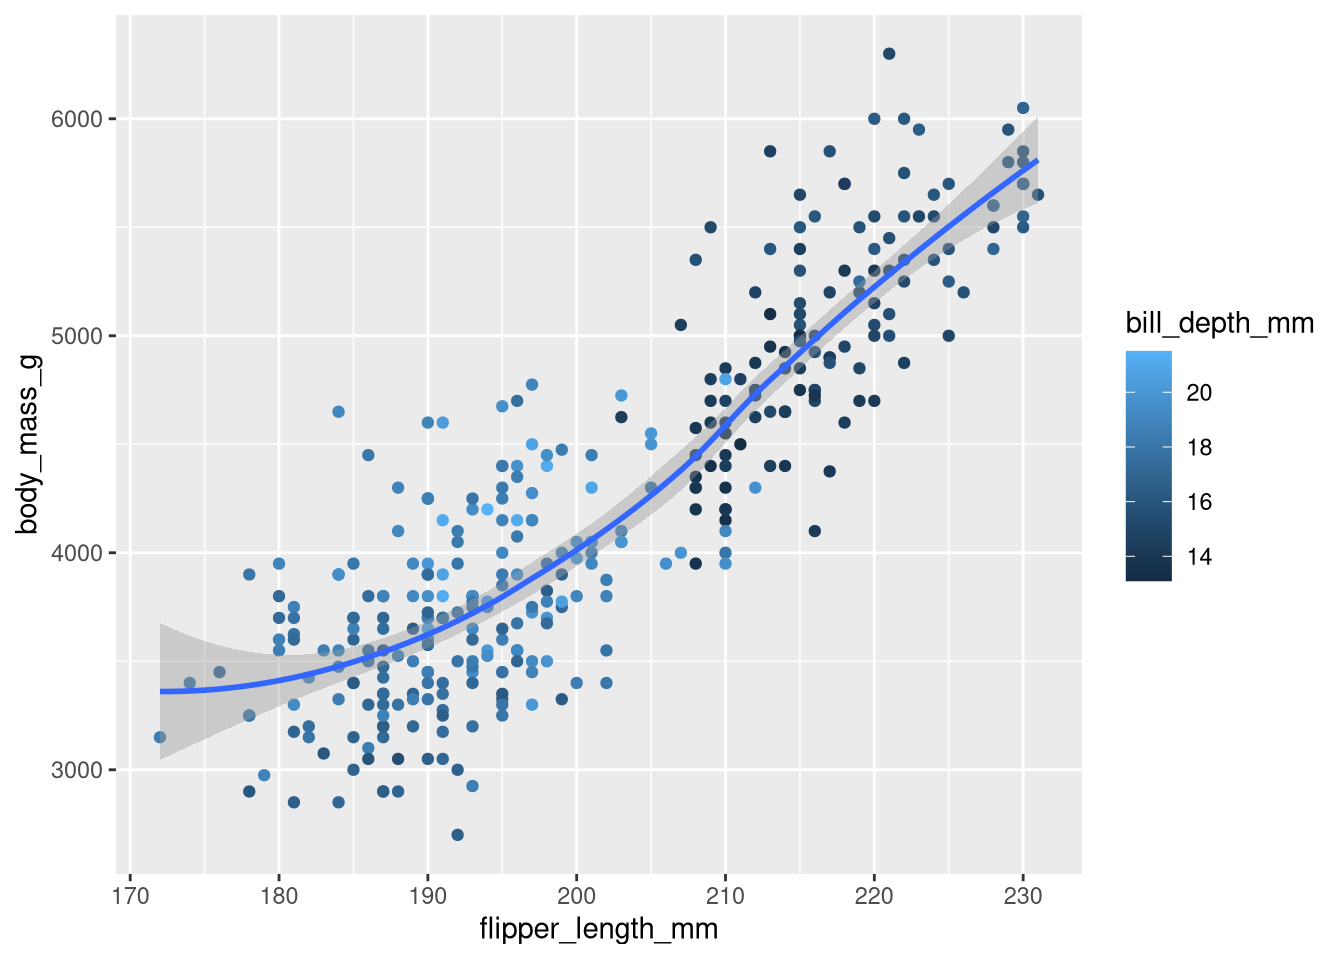
\includegraphics{CH01_files/figure-pdf/unnamed-chunk-9-1.pdf}

  }

  \end{figure}

  \begin{tcolorbox}[enhanced jigsaw, breakable, bottomtitle=1mm, left=2mm, colback=white, toprule=.15mm, leftrule=.75mm, colframe=quarto-callout-note-color-frame, colbacktitle=quarto-callout-note-color!10!white, title={Answer}, coltitle=black, toptitle=1mm, bottomrule=.15mm, opacitybacktitle=0.6, arc=.35mm, rightrule=.15mm, titlerule=0mm, opacityback=0]

\begin{Shaded}
\begin{Highlighting}[]
\CommentTok{\# Your R Code here}
\end{Highlighting}
\end{Shaded}

  \emph{Your answer here.}

  \end{tcolorbox}
\item
  Run this code in your head and predict what the output will look like.
  Then, run the code in R and check your predictions.

\begin{Shaded}
\begin{Highlighting}[]
\FunctionTok{ggplot}\NormalTok{(}
  \AttributeTok{data =}\NormalTok{ penguins,}
  \AttributeTok{mapping =} \FunctionTok{aes}\NormalTok{(}\AttributeTok{x =}\NormalTok{ flipper\_length\_mm, }\AttributeTok{y =}\NormalTok{ body\_mass\_g, }\AttributeTok{color =}\NormalTok{ island)}
\NormalTok{) }\SpecialCharTok{+}
    \FunctionTok{geom\_point}\NormalTok{() }\SpecialCharTok{+}
    \FunctionTok{geom\_smooth}\NormalTok{(}\AttributeTok{se =} \ConstantTok{FALSE}\NormalTok{)}
\end{Highlighting}
\end{Shaded}

  \begin{tcolorbox}[enhanced jigsaw, breakable, bottomtitle=1mm, left=2mm, colback=white, toprule=.15mm, leftrule=.75mm, colframe=quarto-callout-note-color-frame, colbacktitle=quarto-callout-note-color!10!white, title={Answer}, coltitle=black, toptitle=1mm, bottomrule=.15mm, opacitybacktitle=0.6, arc=.35mm, rightrule=.15mm, titlerule=0mm, opacityback=0]

  \emph{Your answer here.}

\begin{Shaded}
\begin{Highlighting}[]
\CommentTok{\# Your R code here}
\end{Highlighting}
\end{Shaded}

  \end{tcolorbox}
\item
  Will these two graphs look different? Why/why not?

\begin{Shaded}
\begin{Highlighting}[]
\FunctionTok{ggplot}\NormalTok{(}
  \AttributeTok{data =}\NormalTok{ penguins,}
  \AttributeTok{mapping =} \FunctionTok{aes}\NormalTok{(}\AttributeTok{x =}\NormalTok{ flipper\_length\_mm, }\AttributeTok{y =}\NormalTok{ body\_mass\_g)}
\NormalTok{) }\SpecialCharTok{+}
  \FunctionTok{geom\_point}\NormalTok{() }\SpecialCharTok{+}
  \FunctionTok{geom\_smooth}\NormalTok{()}

\FunctionTok{ggplot}\NormalTok{() }\SpecialCharTok{+}
  \FunctionTok{geom\_point}\NormalTok{(}
    \AttributeTok{data =}\NormalTok{ penguins,}
    \AttributeTok{mapping =} \FunctionTok{aes}\NormalTok{(}\AttributeTok{x =}\NormalTok{ flipper\_length\_mm, }\AttributeTok{y =}\NormalTok{ body\_mass\_g)}
\NormalTok{  ) }\SpecialCharTok{+}
  \FunctionTok{geom\_smooth}\NormalTok{(}
    \AttributeTok{data =}\NormalTok{ penguins,}
    \AttributeTok{mapping =} \FunctionTok{aes}\NormalTok{(}\AttributeTok{x =}\NormalTok{ flipper\_length\_mm, }\AttributeTok{y =}\NormalTok{ body\_mass\_g)}
\NormalTok{  )}
\end{Highlighting}
\end{Shaded}

  \begin{tcolorbox}[enhanced jigsaw, breakable, bottomtitle=1mm, left=2mm, colback=white, toprule=.15mm, leftrule=.75mm, colframe=quarto-callout-note-color-frame, colbacktitle=quarto-callout-note-color!10!white, title={Answer}, coltitle=black, toptitle=1mm, bottomrule=.15mm, opacitybacktitle=0.6, arc=.35mm, rightrule=.15mm, titlerule=0mm, opacityback=0]

  \emph{Your answer here.}

\begin{Shaded}
\begin{Highlighting}[]
\FunctionTok{library}\NormalTok{(patchwork)}
\CommentTok{\# Your R code here}
\end{Highlighting}
\end{Shaded}

  \end{tcolorbox}
\item
  Make a bar plot of \texttt{species} of \texttt{penguins}, where you
  assign \texttt{species} to the \texttt{y} aesthetic. How is this plot
  different?

  \begin{tcolorbox}[enhanced jigsaw, breakable, bottomtitle=1mm, left=2mm, colback=white, toprule=.15mm, leftrule=.75mm, colframe=quarto-callout-note-color-frame, colbacktitle=quarto-callout-note-color!10!white, title={Answer}, coltitle=black, toptitle=1mm, bottomrule=.15mm, opacitybacktitle=0.6, arc=.35mm, rightrule=.15mm, titlerule=0mm, opacityback=0]

  \emph{Your answer here.}

\begin{Shaded}
\begin{Highlighting}[]
\CommentTok{\# Your R code here}
\end{Highlighting}
\end{Shaded}

  \end{tcolorbox}
\item
  How are the following two plots different? Which aesthetic,
  \texttt{color} or \texttt{fill}, is more useful for changing the color
  of bars?

\begin{Shaded}
\begin{Highlighting}[]
\FunctionTok{ggplot}\NormalTok{(penguins, }\FunctionTok{aes}\NormalTok{(}\AttributeTok{x =}\NormalTok{ species)) }\SpecialCharTok{+}
  \FunctionTok{geom\_bar}\NormalTok{(}\AttributeTok{color =} \StringTok{"red"}\NormalTok{)}

\FunctionTok{ggplot}\NormalTok{(penguins, }\FunctionTok{aes}\NormalTok{(}\AttributeTok{x =}\NormalTok{ species)) }\SpecialCharTok{+}
  \FunctionTok{geom\_bar}\NormalTok{(}\AttributeTok{fill =} \StringTok{"red"}\NormalTok{)}
\end{Highlighting}
\end{Shaded}

  \begin{tcolorbox}[enhanced jigsaw, breakable, bottomtitle=1mm, left=2mm, colback=white, toprule=.15mm, leftrule=.75mm, colframe=quarto-callout-note-color-frame, colbacktitle=quarto-callout-note-color!10!white, title={Answer}, coltitle=black, toptitle=1mm, bottomrule=.15mm, opacitybacktitle=0.6, arc=.35mm, rightrule=.15mm, titlerule=0mm, opacityback=0]

\begin{Shaded}
\begin{Highlighting}[]
\FunctionTok{ggplot}\NormalTok{(penguins, }\FunctionTok{aes}\NormalTok{(}\AttributeTok{x =}\NormalTok{ species)) }\SpecialCharTok{+}
    \FunctionTok{geom\_bar}\NormalTok{(}\AttributeTok{color =} \StringTok{"red"}\NormalTok{) }\OtherTok{{-}\textgreater{}}\NormalTok{ p1}

\FunctionTok{ggplot}\NormalTok{(penguins, }\FunctionTok{aes}\NormalTok{(}\AttributeTok{x =}\NormalTok{ species)) }\SpecialCharTok{+}
  \FunctionTok{geom\_bar}\NormalTok{(}\AttributeTok{fill =} \StringTok{"red"}\NormalTok{) }\OtherTok{{-}\textgreater{}}\NormalTok{ p2}
\NormalTok{p1 }\SpecialCharTok{+}\NormalTok{ p2}
\end{Highlighting}
\end{Shaded}

  \begin{figure}[H]

  {\centering 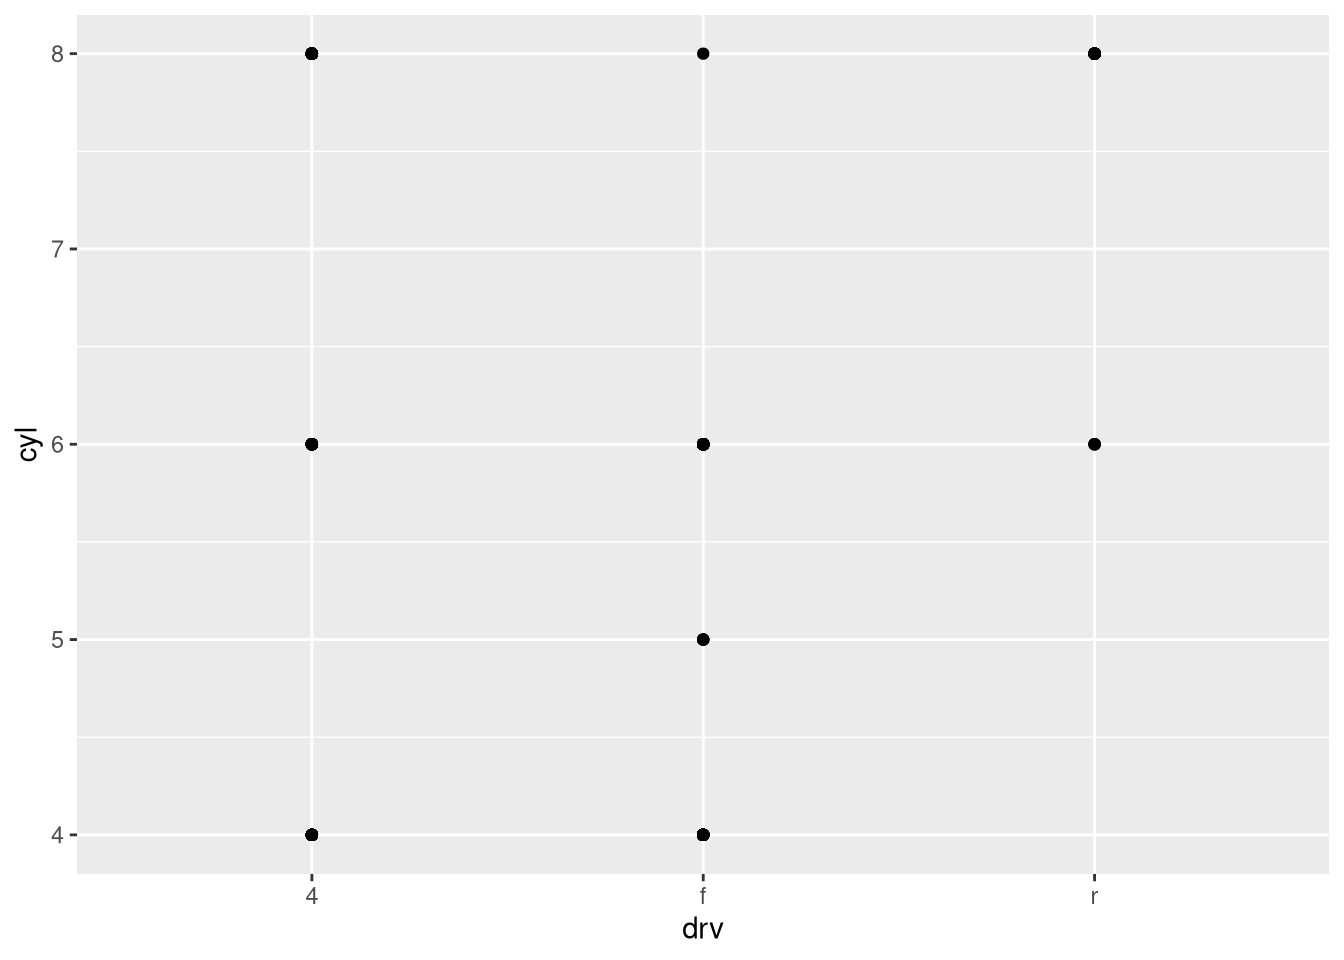
\includegraphics{CH01_files/figure-pdf/unnamed-chunk-17-1.pdf}

  }

  \end{figure}

  \emph{Your answer here.}

  \end{tcolorbox}
\item
  What does the \texttt{bins} argument in \texttt{geom\_histogram()} do?

  \begin{tcolorbox}[enhanced jigsaw, breakable, bottomtitle=1mm, left=2mm, colback=white, toprule=.15mm, leftrule=.75mm, colframe=quarto-callout-note-color-frame, colbacktitle=quarto-callout-note-color!10!white, title={Answer}, coltitle=black, toptitle=1mm, bottomrule=.15mm, opacitybacktitle=0.6, arc=.35mm, rightrule=.15mm, titlerule=0mm, opacityback=0]

  \emph{Your answer here.}

  \end{tcolorbox}
\item
  Make a histogram of the \texttt{carat} variable in the
  \texttt{diamonds} dataset that is available when you load the
  \texttt{tidyverse} package. Experiment with different binwidths. What
  binwidth reveals the most interesting patterns?

  \begin{tcolorbox}[enhanced jigsaw, breakable, bottomtitle=1mm, left=2mm, colback=white, toprule=.15mm, leftrule=.75mm, colframe=quarto-callout-note-color-frame, colbacktitle=quarto-callout-note-color!10!white, title={Answer}, coltitle=black, toptitle=1mm, bottomrule=.15mm, opacitybacktitle=0.6, arc=.35mm, rightrule=.15mm, titlerule=0mm, opacityback=0]

\begin{Shaded}
\begin{Highlighting}[]
\CommentTok{\# Your R code here}
\end{Highlighting}
\end{Shaded}

  \emph{Your answer here.}

  \end{tcolorbox}
\item
  The \texttt{mpg} data frame that is bundled with the \texttt{ggplot2}
  package contains 234 observations collected by the US Environmental
  Protection Agency on 38 car models. Which variables in \texttt{mpg}
  are categorical? Which variables are numerical? (Hint: Type
  \texttt{?mpg} to read the documentation for the dataset.) How can you
  see this information when you run \texttt{mpg}?

  \begin{tcolorbox}[enhanced jigsaw, breakable, bottomtitle=1mm, left=2mm, colback=white, toprule=.15mm, leftrule=.75mm, colframe=quarto-callout-note-color-frame, colbacktitle=quarto-callout-note-color!10!white, title={Answer}, coltitle=black, toptitle=1mm, bottomrule=.15mm, opacitybacktitle=0.6, arc=.35mm, rightrule=.15mm, titlerule=0mm, opacityback=0]

\begin{Shaded}
\begin{Highlighting}[]
\CommentTok{\# Your R code here}
\end{Highlighting}
\end{Shaded}

  \emph{Your answer here.}

  \end{tcolorbox}
\item
  Make a scatterplot of \texttt{hwy} vs.~\texttt{displ} using the
  \texttt{mpg} data frame. Next, map a third, numerical variable to
  \texttt{color}, then \texttt{size}, then both \texttt{color} and
  \texttt{size}, then \texttt{shape}. How do these aesthetics behave
  differently for categorical vs.~numerical variables?

  \begin{tcolorbox}[enhanced jigsaw, breakable, bottomtitle=1mm, left=2mm, colback=white, toprule=.15mm, leftrule=.75mm, colframe=quarto-callout-note-color-frame, colbacktitle=quarto-callout-note-color!10!white, title={Answer}, coltitle=black, toptitle=1mm, bottomrule=.15mm, opacitybacktitle=0.6, arc=.35mm, rightrule=.15mm, titlerule=0mm, opacityback=0]

\begin{Shaded}
\begin{Highlighting}[]
\CommentTok{\# Your R code here}
\end{Highlighting}
\end{Shaded}

  \emph{Your answer here.}

  \end{tcolorbox}
\item
  In the scatterplot of \texttt{hwy} vs.~\texttt{displ}, what happens if
  you map a third variable to \texttt{linewidth}?

  \begin{tcolorbox}[enhanced jigsaw, breakable, bottomtitle=1mm, left=2mm, colback=white, toprule=.15mm, leftrule=.75mm, colframe=quarto-callout-note-color-frame, colbacktitle=quarto-callout-note-color!10!white, title={Answer}, coltitle=black, toptitle=1mm, bottomrule=.15mm, opacitybacktitle=0.6, arc=.35mm, rightrule=.15mm, titlerule=0mm, opacityback=0]

\begin{Shaded}
\begin{Highlighting}[]
\CommentTok{\# Your R code here}
\end{Highlighting}
\end{Shaded}

  \emph{Your answer here.}

  \end{tcolorbox}
\item
  What happens if you map the same variable to multiple aesthetics?

  \begin{tcolorbox}[enhanced jigsaw, breakable, bottomtitle=1mm, left=2mm, colback=white, toprule=.15mm, leftrule=.75mm, colframe=quarto-callout-note-color-frame, colbacktitle=quarto-callout-note-color!10!white, title={Answer}, coltitle=black, toptitle=1mm, bottomrule=.15mm, opacitybacktitle=0.6, arc=.35mm, rightrule=.15mm, titlerule=0mm, opacityback=0]

\begin{Shaded}
\begin{Highlighting}[]
\CommentTok{\# Your R code here}
\end{Highlighting}
\end{Shaded}

  \emph{Your answer here.}

  \end{tcolorbox}
\item
  Make a scatterplot of \texttt{bill\_depth\_mm}
  vs.~\texttt{bill\_length\_mm} and color the points by
  \texttt{species}. What does adding coloring by species reveal about
  the relationship between these two variables? What about faceting by
  \texttt{species}?

  \begin{tcolorbox}[enhanced jigsaw, breakable, bottomtitle=1mm, left=2mm, colback=white, toprule=.15mm, leftrule=.75mm, colframe=quarto-callout-note-color-frame, colbacktitle=quarto-callout-note-color!10!white, title={Answer}, coltitle=black, toptitle=1mm, bottomrule=.15mm, opacitybacktitle=0.6, arc=.35mm, rightrule=.15mm, titlerule=0mm, opacityback=0]

\begin{Shaded}
\begin{Highlighting}[]
\CommentTok{\# Your R code here}
\end{Highlighting}
\end{Shaded}

  \emph{Your answer here.}

  \end{tcolorbox}
\item
  Why does the following yield two separate legends? How would you fix
  it to combine the two legends?

\begin{Shaded}
\begin{Highlighting}[]
\FunctionTok{ggplot}\NormalTok{(}
  \AttributeTok{data =}\NormalTok{ penguins,}
  \AttributeTok{mapping =} \FunctionTok{aes}\NormalTok{(}
    \AttributeTok{x =}\NormalTok{ bill\_length\_mm, }\AttributeTok{y =}\NormalTok{ bill\_depth\_mm, }
    \AttributeTok{color =}\NormalTok{ species, }\AttributeTok{shape =}\NormalTok{ species}
\NormalTok{  )}
\NormalTok{) }\SpecialCharTok{+}
  \FunctionTok{geom\_point}\NormalTok{() }\SpecialCharTok{+}
  \FunctionTok{labs}\NormalTok{(}\AttributeTok{color =} \StringTok{"Species"}\NormalTok{)}
\end{Highlighting}
\end{Shaded}

  \begin{tcolorbox}[enhanced jigsaw, breakable, bottomtitle=1mm, left=2mm, colback=white, toprule=.15mm, leftrule=.75mm, colframe=quarto-callout-note-color-frame, colbacktitle=quarto-callout-note-color!10!white, title={Answer}, coltitle=black, toptitle=1mm, bottomrule=.15mm, opacitybacktitle=0.6, arc=.35mm, rightrule=.15mm, titlerule=0mm, opacityback=0]

\begin{Shaded}
\begin{Highlighting}[]
\CommentTok{\# Your R fix here}
\end{Highlighting}
\end{Shaded}

  \emph{Your answer here.}

  \end{tcolorbox}
\item
  Create the two following stacked bar plots. Which question can you
  answer with the first one? Which question can you answer with the
  second one?

\begin{Shaded}
\begin{Highlighting}[]
\FunctionTok{ggplot}\NormalTok{(penguins, }\FunctionTok{aes}\NormalTok{(}\AttributeTok{x =}\NormalTok{ island, }\AttributeTok{fill =}\NormalTok{ species)) }\SpecialCharTok{+}
  \FunctionTok{geom\_bar}\NormalTok{(}\AttributeTok{position =} \StringTok{"fill"}\NormalTok{)}
\end{Highlighting}
\end{Shaded}

\begin{Shaded}
\begin{Highlighting}[]
\FunctionTok{ggplot}\NormalTok{(penguins, }\FunctionTok{aes}\NormalTok{(}\AttributeTok{x =}\NormalTok{ species, }\AttributeTok{fill =}\NormalTok{ island)) }\SpecialCharTok{+}
  \FunctionTok{geom\_bar}\NormalTok{(}\AttributeTok{position =} \StringTok{"fill"}\NormalTok{)}
\end{Highlighting}
\end{Shaded}

  \begin{tcolorbox}[enhanced jigsaw, breakable, bottomtitle=1mm, left=2mm, colback=white, toprule=.15mm, leftrule=.75mm, colframe=quarto-callout-note-color-frame, colbacktitle=quarto-callout-note-color!10!white, title={Answer}, coltitle=black, toptitle=1mm, bottomrule=.15mm, opacitybacktitle=0.6, arc=.35mm, rightrule=.15mm, titlerule=0mm, opacityback=0]

\begin{Shaded}
\begin{Highlighting}[]
\FunctionTok{ggplot}\NormalTok{(penguins, }\FunctionTok{aes}\NormalTok{(}\AttributeTok{x =}\NormalTok{ island, }\AttributeTok{fill =}\NormalTok{ species)) }\SpecialCharTok{+}
  \FunctionTok{geom\_bar}\NormalTok{(}\AttributeTok{position =} \StringTok{"fill"}\NormalTok{) }\OtherTok{{-}\textgreater{}}\NormalTok{ p1}
\FunctionTok{ggplot}\NormalTok{(penguins, }\FunctionTok{aes}\NormalTok{(}\AttributeTok{x =}\NormalTok{ species, }\AttributeTok{fill =}\NormalTok{ island)) }\SpecialCharTok{+}
  \FunctionTok{geom\_bar}\NormalTok{(}\AttributeTok{position =} \StringTok{"fill"}\NormalTok{) }\OtherTok{{-}\textgreater{}}\NormalTok{ p2}
\NormalTok{p1 }\SpecialCharTok{/}\NormalTok{ p2}
\end{Highlighting}
\end{Shaded}

  \begin{figure}[H]

  {\centering \includegraphics{CH01_files/figure-pdf/unnamed-chunk-27-1.pdf}

  }

  \end{figure}

  \emph{Your answer here.}

  \end{tcolorbox}
\item
  Run the following lines of code. Which of the two plots is saved as
  \texttt{mpg-plot.png}? Why?

\begin{Shaded}
\begin{Highlighting}[]
\FunctionTok{ggplot}\NormalTok{(mpg, }\FunctionTok{aes}\NormalTok{(}\AttributeTok{x =}\NormalTok{ class)) }\SpecialCharTok{+}
  \FunctionTok{geom\_bar}\NormalTok{()}
\FunctionTok{ggplot}\NormalTok{(mpg, }\FunctionTok{aes}\NormalTok{(}\AttributeTok{x =}\NormalTok{ cty, }\AttributeTok{y =}\NormalTok{ hwy)) }\SpecialCharTok{+}
  \FunctionTok{geom\_point}\NormalTok{()}
\FunctionTok{ggsave}\NormalTok{(}\StringTok{"mpg{-}plot.png"}\NormalTok{)}
\end{Highlighting}
\end{Shaded}

  \begin{tcolorbox}[enhanced jigsaw, breakable, bottomtitle=1mm, left=2mm, colback=white, toprule=.15mm, leftrule=.75mm, colframe=quarto-callout-note-color-frame, colbacktitle=quarto-callout-note-color!10!white, title={Answer}, coltitle=black, toptitle=1mm, bottomrule=.15mm, opacitybacktitle=0.6, arc=.35mm, rightrule=.15mm, titlerule=0mm, opacityback=0]

\begin{Shaded}
\begin{Highlighting}[]
\CommentTok{\# Your R code here}
\end{Highlighting}
\end{Shaded}

  \emph{Your answer here.}

  \end{tcolorbox}
\item
  What do you need to change in the code above to save the plot as a PDF
  instead of a PNG? How could you find out what types of image files
  would work in \texttt{ggsave()}?

  \begin{tcolorbox}[enhanced jigsaw, breakable, bottomtitle=1mm, left=2mm, colback=white, toprule=.15mm, leftrule=.75mm, colframe=quarto-callout-note-color-frame, colbacktitle=quarto-callout-note-color!10!white, title={Answer}, coltitle=black, toptitle=1mm, bottomrule=.15mm, opacitybacktitle=0.6, arc=.35mm, rightrule=.15mm, titlerule=0mm, opacityback=0]

  \emph{Your answer here.}

  \end{tcolorbox}
\end{enumerate}

\bookmarksetup{startatroot}

\hypertarget{exercises-chapter-2}{%
\chapter{Exercises (Chapter 2)}\label{exercises-chapter-2}}

\begin{enumerate}
\def\labelenumi{\arabic{enumi}.}
\item
  Why does this code not work?

\begin{Shaded}
\begin{Highlighting}[]
\NormalTok{my\_variable }\OtherTok{\textless{}{-}} \DecValTok{10}
\NormalTok{my\_varıable}
\end{Highlighting}
\end{Shaded}

  Look carefully! (This may seem like an exercise in pointlessness, but
  training your brain to notice even the tiniest difference will pay off
  when programming.)

  \begin{tcolorbox}[enhanced jigsaw, breakable, bottomtitle=1mm, left=2mm, colback=white, toprule=.15mm, leftrule=.75mm, colframe=quarto-callout-note-color-frame, colbacktitle=quarto-callout-note-color!10!white, title={Answer}, coltitle=black, toptitle=1mm, bottomrule=.15mm, opacitybacktitle=0.6, arc=.35mm, rightrule=.15mm, titlerule=0mm, opacityback=0]

  \emph{Your answer here.}

  \end{tcolorbox}
\item
  Tweak each of the following R commands so that they run correctly:

\begin{Shaded}
\begin{Highlighting}[]
\FunctionTok{libary}\NormalTok{(todyverse)}
\FunctionTok{ggplot}\NormalTok{(}\AttributeTok{dTA =}\NormalTok{ mpg) }\SpecialCharTok{+} 
  \FunctionTok{geom\_point}\NormalTok{(}\AttributeTok{maping =} \FunctionTok{aes}\NormalTok{(}\AttributeTok{x =}\NormalTok{ displ }\AttributeTok{y =}\NormalTok{ hwy)) }\SpecialCharTok{+}
  \FunctionTok{geom\_smooth}\NormalTok{(}\AttributeTok{method =} \StringTok{"lm)}
\end{Highlighting}
\end{Shaded}

  \begin{tcolorbox}[enhanced jigsaw, breakable, bottomtitle=1mm, left=2mm, colback=white, toprule=.15mm, leftrule=.75mm, colframe=quarto-callout-note-color-frame, colbacktitle=quarto-callout-note-color!10!white, title={Answer}, coltitle=black, toptitle=1mm, bottomrule=.15mm, opacitybacktitle=0.6, arc=.35mm, rightrule=.15mm, titlerule=0mm, opacityback=0]

\begin{Shaded}
\begin{Highlighting}[]
\CommentTok{\# Your R code here}
\end{Highlighting}
\end{Shaded}

  \end{tcolorbox}
\item
  Press Option + Shift + K / Alt + Shift + K. What happens? How can you
  get to the same place using the menus?

  \begin{tcolorbox}[enhanced jigsaw, breakable, bottomtitle=1mm, left=2mm, colback=white, toprule=.15mm, leftrule=.75mm, colframe=quarto-callout-note-color-frame, colbacktitle=quarto-callout-note-color!10!white, title={Answer}, coltitle=black, toptitle=1mm, bottomrule=.15mm, opacitybacktitle=0.6, arc=.35mm, rightrule=.15mm, titlerule=0mm, opacityback=0]

  \emph{Your answer here.}

  \end{tcolorbox}
\item
  Let's revisit an exercise from ``Saving Your Plots''. Run the
  following lines of code. Which of the two plots is saved as
  \texttt{mpg-plot.png}? Why?

\begin{Shaded}
\begin{Highlighting}[]
\NormalTok{my\_bar\_plot }\OtherTok{\textless{}{-}} \FunctionTok{ggplot}\NormalTok{(mpg, }\FunctionTok{aes}\NormalTok{(}\AttributeTok{x =}\NormalTok{ class)) }\SpecialCharTok{+}
  \FunctionTok{geom\_bar}\NormalTok{()}
\NormalTok{my\_scatter\_plot }\OtherTok{\textless{}{-}} \FunctionTok{ggplot}\NormalTok{(mpg, }\FunctionTok{aes}\NormalTok{(}\AttributeTok{x =}\NormalTok{ cty, }\AttributeTok{y =}\NormalTok{ hwy)) }\SpecialCharTok{+}
  \FunctionTok{geom\_point}\NormalTok{()}
\FunctionTok{ggsave}\NormalTok{(}\AttributeTok{filename =} \StringTok{"mpg{-}plot.png"}\NormalTok{, }\AttributeTok{plot =}\NormalTok{ my\_bar\_plot)}
\end{Highlighting}
\end{Shaded}

  \begin{tcolorbox}[enhanced jigsaw, breakable, bottomtitle=1mm, left=2mm, colback=white, toprule=.15mm, leftrule=.75mm, colframe=quarto-callout-note-color-frame, colbacktitle=quarto-callout-note-color!10!white, title={Answer}, coltitle=black, toptitle=1mm, bottomrule=.15mm, opacitybacktitle=0.6, arc=.35mm, rightrule=.15mm, titlerule=0mm, opacityback=0]

\begin{Shaded}
\begin{Highlighting}[]
\NormalTok{my\_bar\_plot }\OtherTok{\textless{}{-}} \FunctionTok{ggplot}\NormalTok{(mpg, }\FunctionTok{aes}\NormalTok{(}\AttributeTok{x =}\NormalTok{ class)) }\SpecialCharTok{+}
  \FunctionTok{geom\_bar}\NormalTok{()}
\NormalTok{my\_scatter\_plot }\OtherTok{\textless{}{-}} \FunctionTok{ggplot}\NormalTok{(mpg, }\FunctionTok{aes}\NormalTok{(}\AttributeTok{x =}\NormalTok{ cty, }\AttributeTok{y =}\NormalTok{ hwy)) }\SpecialCharTok{+}
  \FunctionTok{geom\_point}\NormalTok{()}
\FunctionTok{ggsave}\NormalTok{(}\AttributeTok{filename =} \StringTok{"mpg{-}plot.png"}\NormalTok{, }\AttributeTok{plot =}\NormalTok{ my\_bar\_plot)}
\end{Highlighting}
\end{Shaded}

\begin{verbatim}
Saving 5.5 x 3.5 in image
\end{verbatim}

  \emph{Your answer here.}

  \end{tcolorbox}
\end{enumerate}

\bookmarksetup{startatroot}

\hypertarget{exercises-chapter-3}{%
\chapter{Exercises (Chapter 3)}\label{exercises-chapter-3}}

\begin{enumerate}
\def\labelenumi{\arabic{enumi}.}
\item
  In a single pipeline for each condition, find all flights that meet
  the condition:

  \begin{itemize}
  \item
    Had an arrival delay of two or more hours

    \begin{tcolorbox}[enhanced jigsaw, breakable, bottomtitle=1mm, left=2mm, colback=white, toprule=.15mm, leftrule=.75mm, colframe=quarto-callout-note-color-frame, colbacktitle=quarto-callout-note-color!10!white, title={Answer}, coltitle=black, toptitle=1mm, bottomrule=.15mm, opacitybacktitle=0.6, arc=.35mm, rightrule=.15mm, titlerule=0mm, opacityback=0]

\begin{Shaded}
\begin{Highlighting}[]
\FunctionTok{library}\NormalTok{(tidyverse)}
\FunctionTok{library}\NormalTok{(nycflights13)}
\CommentTok{\# Your code here}
\end{Highlighting}
\end{Shaded}

    \end{tcolorbox}
  \item
    Flew to Houston (\texttt{IAH} or \texttt{HOU})

    \begin{tcolorbox}[enhanced jigsaw, breakable, bottomtitle=1mm, left=2mm, colback=white, toprule=.15mm, leftrule=.75mm, colframe=quarto-callout-note-color-frame, colbacktitle=quarto-callout-note-color!10!white, title={Answer}, coltitle=black, toptitle=1mm, bottomrule=.15mm, opacitybacktitle=0.6, arc=.35mm, rightrule=.15mm, titlerule=0mm, opacityback=0]

\begin{Shaded}
\begin{Highlighting}[]
\CommentTok{\# Your code here}
\end{Highlighting}
\end{Shaded}

    \end{tcolorbox}
  \item
    Were operated by United, American, or Delta

    \begin{tcolorbox}[enhanced jigsaw, breakable, bottomtitle=1mm, left=2mm, colback=white, toprule=.15mm, leftrule=.75mm, colframe=quarto-callout-note-color-frame, colbacktitle=quarto-callout-note-color!10!white, title={Answer}, coltitle=black, toptitle=1mm, bottomrule=.15mm, opacitybacktitle=0.6, arc=.35mm, rightrule=.15mm, titlerule=0mm, opacityback=0]

\begin{Shaded}
\begin{Highlighting}[]
\CommentTok{\# Your code here}
\end{Highlighting}
\end{Shaded}

    \end{tcolorbox}
  \item
    Departed in summer (July, August, and September)

    \begin{tcolorbox}[enhanced jigsaw, breakable, bottomtitle=1mm, left=2mm, colback=white, toprule=.15mm, leftrule=.75mm, colframe=quarto-callout-note-color-frame, colbacktitle=quarto-callout-note-color!10!white, title={Answer}, coltitle=black, toptitle=1mm, bottomrule=.15mm, opacitybacktitle=0.6, arc=.35mm, rightrule=.15mm, titlerule=0mm, opacityback=0]

\begin{Shaded}
\begin{Highlighting}[]
\CommentTok{\# Your code here}
\end{Highlighting}
\end{Shaded}

    \end{tcolorbox}
  \item
    Arrived more than two hours late, but didn't leave late.

    \begin{tcolorbox}[enhanced jigsaw, breakable, bottomtitle=1mm, left=2mm, colback=white, toprule=.15mm, leftrule=.75mm, colframe=quarto-callout-note-color-frame, colbacktitle=quarto-callout-note-color!10!white, title={Answer}, coltitle=black, toptitle=1mm, bottomrule=.15mm, opacitybacktitle=0.6, arc=.35mm, rightrule=.15mm, titlerule=0mm, opacityback=0]

\begin{Shaded}
\begin{Highlighting}[]
\CommentTok{\# Your code here}
\end{Highlighting}
\end{Shaded}

    \end{tcolorbox}
  \item
    Were delayed by at least an hour, but made up over 30 minutes in
    flight

    \begin{tcolorbox}[enhanced jigsaw, breakable, bottomtitle=1mm, left=2mm, colback=white, toprule=.15mm, leftrule=.75mm, colframe=quarto-callout-note-color-frame, colbacktitle=quarto-callout-note-color!10!white, title={Answer}, coltitle=black, toptitle=1mm, bottomrule=.15mm, opacitybacktitle=0.6, arc=.35mm, rightrule=.15mm, titlerule=0mm, opacityback=0]

\begin{Shaded}
\begin{Highlighting}[]
\CommentTok{\# Your code here}
\end{Highlighting}
\end{Shaded}

    \end{tcolorbox}
  \end{itemize}
\item
  Sort \texttt{flights} to find the flights with longest departure
  delays. Find the flights that left earliest in the morning.

  \begin{tcolorbox}[enhanced jigsaw, breakable, bottomtitle=1mm, left=2mm, colback=white, toprule=.15mm, leftrule=.75mm, colframe=quarto-callout-note-color-frame, colbacktitle=quarto-callout-note-color!10!white, title={Answer}, coltitle=black, toptitle=1mm, bottomrule=.15mm, opacitybacktitle=0.6, arc=.35mm, rightrule=.15mm, titlerule=0mm, opacityback=0]

\begin{Shaded}
\begin{Highlighting}[]
\CommentTok{\# Your code here}
\end{Highlighting}
\end{Shaded}

  \end{tcolorbox}
\item
  Sort \texttt{flights} to find the fastest flights. (Hint: Try
  including a math calculation inside of your function.)

  \begin{tcolorbox}[enhanced jigsaw, breakable, bottomtitle=1mm, left=2mm, colback=white, toprule=.15mm, leftrule=.75mm, colframe=quarto-callout-note-color-frame, colbacktitle=quarto-callout-note-color!10!white, title={Answer}, coltitle=black, toptitle=1mm, bottomrule=.15mm, opacitybacktitle=0.6, arc=.35mm, rightrule=.15mm, titlerule=0mm, opacityback=0]

\begin{Shaded}
\begin{Highlighting}[]
\CommentTok{\# Your code here}
\end{Highlighting}
\end{Shaded}

  \end{tcolorbox}
\item
  Was there a flight on every day of 2013?

  \begin{tcolorbox}[enhanced jigsaw, breakable, bottomtitle=1mm, left=2mm, colback=white, toprule=.15mm, leftrule=.75mm, colframe=quarto-callout-note-color-frame, colbacktitle=quarto-callout-note-color!10!white, title={Answer}, coltitle=black, toptitle=1mm, bottomrule=.15mm, opacitybacktitle=0.6, arc=.35mm, rightrule=.15mm, titlerule=0mm, opacityback=0]

\begin{Shaded}
\begin{Highlighting}[]
\CommentTok{\# Your code here}
\end{Highlighting}
\end{Shaded}

  \emph{Your text answer here.}

  \end{tcolorbox}
\item
  Which flights traveled the farthest distance? Which traveled the least
  distance?

  \begin{tcolorbox}[enhanced jigsaw, breakable, bottomtitle=1mm, left=2mm, colback=white, toprule=.15mm, leftrule=.75mm, colframe=quarto-callout-note-color-frame, colbacktitle=quarto-callout-note-color!10!white, title={Answer}, coltitle=black, toptitle=1mm, bottomrule=.15mm, opacitybacktitle=0.6, arc=.35mm, rightrule=.15mm, titlerule=0mm, opacityback=0]

\begin{Shaded}
\begin{Highlighting}[]
\CommentTok{\# Your code here}
\end{Highlighting}
\end{Shaded}

  \end{tcolorbox}
\item
  Does it matter what order you used \texttt{filter()} and
  \texttt{arrange()} if you're using both? Why/why not? Think about the
  results and how much work the functions would have to do.

  \begin{tcolorbox}[enhanced jigsaw, breakable, bottomtitle=1mm, left=2mm, colback=white, toprule=.15mm, leftrule=.75mm, colframe=quarto-callout-note-color-frame, colbacktitle=quarto-callout-note-color!10!white, title={Answer}, coltitle=black, toptitle=1mm, bottomrule=.15mm, opacitybacktitle=0.6, arc=.35mm, rightrule=.15mm, titlerule=0mm, opacityback=0]

  \emph{Your text answer here.}

  \end{tcolorbox}
\item
  Compare \texttt{dep\_time}, \texttt{sched\_dep\_time}, and
  \texttt{dep\_delay}. How would you expect those three numbers to be
  related?

  \begin{tcolorbox}[enhanced jigsaw, breakable, bottomtitle=1mm, left=2mm, colback=white, toprule=.15mm, leftrule=.75mm, colframe=quarto-callout-note-color-frame, colbacktitle=quarto-callout-note-color!10!white, title={Answer}, coltitle=black, toptitle=1mm, bottomrule=.15mm, opacitybacktitle=0.6, arc=.35mm, rightrule=.15mm, titlerule=0mm, opacityback=0]

\begin{Shaded}
\begin{Highlighting}[]
\CommentTok{\# Your code here}
\end{Highlighting}
\end{Shaded}

  \emph{Your text answer here.}

  \end{tcolorbox}
\item
  Brainstorm as many ways as possible to select \texttt{dep\_time},
  \texttt{dep\_delay}, \texttt{arr\_time}, and \texttt{arr\_delay} from
  \texttt{flights}.

  \begin{tcolorbox}[enhanced jigsaw, breakable, bottomtitle=1mm, left=2mm, colback=white, toprule=.15mm, leftrule=.75mm, colframe=quarto-callout-note-color-frame, colbacktitle=quarto-callout-note-color!10!white, title={Answer}, coltitle=black, toptitle=1mm, bottomrule=.15mm, opacitybacktitle=0.6, arc=.35mm, rightrule=.15mm, titlerule=0mm, opacityback=0]

\begin{Shaded}
\begin{Highlighting}[]
\CommentTok{\# Your code here}
\end{Highlighting}
\end{Shaded}

  \end{tcolorbox}
\item
  What happens if you specify the name of the same variable multiple
  times in a \texttt{select()} call?

  \begin{tcolorbox}[enhanced jigsaw, breakable, bottomtitle=1mm, left=2mm, colback=white, toprule=.15mm, leftrule=.75mm, colframe=quarto-callout-note-color-frame, colbacktitle=quarto-callout-note-color!10!white, title={Answer}, coltitle=black, toptitle=1mm, bottomrule=.15mm, opacitybacktitle=0.6, arc=.35mm, rightrule=.15mm, titlerule=0mm, opacityback=0]

\begin{Shaded}
\begin{Highlighting}[]
\CommentTok{\# Your code here}
\end{Highlighting}
\end{Shaded}

  \emph{Your text answer here.}

  \end{tcolorbox}
\item
  What does the \texttt{any\_of()} function do? Why might it be helpful
  in conjunction with this vector?

\begin{Shaded}
\begin{Highlighting}[]
\NormalTok{variables }\OtherTok{\textless{}{-}} \FunctionTok{c}\NormalTok{(}\StringTok{"year"}\NormalTok{, }\StringTok{"month"}\NormalTok{, }\StringTok{"day"}\NormalTok{, }\StringTok{"dep\_delay"}\NormalTok{, }\StringTok{"arr\_delay"}\NormalTok{)}
\CommentTok{\# Try below first}
\NormalTok{flights }\SpecialCharTok{|\textgreater{}} 
  \FunctionTok{select}\NormalTok{(variables)}
\end{Highlighting}
\end{Shaded}

\begin{verbatim}
Warning: Using an external vector in selections was deprecated in tidyselect 1.1.0.
i Please use `all_of()` or `any_of()` instead.
  # Was:
  data %>% select(variables)

  # Now:
  data %>% select(all_of(variables))

See <https://tidyselect.r-lib.org/reference/faq-external-vector.html>.
\end{verbatim}

\begin{verbatim}
# A tibble: 336,776 x 5
    year month   day dep_delay arr_delay
   <int> <int> <int>     <dbl>     <dbl>
 1  2013     1     1         2        11
 2  2013     1     1         4        20
 3  2013     1     1         2        33
 4  2013     1     1        -1       -18
 5  2013     1     1        -6       -25
 6  2013     1     1        -4        12
 7  2013     1     1        -5        19
 8  2013     1     1        -3       -14
 9  2013     1     1        -3        -8
10  2013     1     1        -2         8
# i 336,766 more rows
\end{verbatim}

\begin{Shaded}
\begin{Highlighting}[]
\CommentTok{\# Or}
\NormalTok{flights }\SpecialCharTok{|\textgreater{}} 
  \FunctionTok{select}\NormalTok{(}\FunctionTok{any\_of}\NormalTok{(variables))}
\end{Highlighting}
\end{Shaded}

\begin{verbatim}
# A tibble: 336,776 x 5
    year month   day dep_delay arr_delay
   <int> <int> <int>     <dbl>     <dbl>
 1  2013     1     1         2        11
 2  2013     1     1         4        20
 3  2013     1     1         2        33
 4  2013     1     1        -1       -18
 5  2013     1     1        -6       -25
 6  2013     1     1        -4        12
 7  2013     1     1        -5        19
 8  2013     1     1        -3       -14
 9  2013     1     1        -3        -8
10  2013     1     1        -2         8
# i 336,766 more rows
\end{verbatim}

  \begin{tcolorbox}[enhanced jigsaw, breakable, bottomtitle=1mm, left=2mm, colback=white, toprule=.15mm, leftrule=.75mm, colframe=quarto-callout-note-color-frame, colbacktitle=quarto-callout-note-color!10!white, title={Answer}, coltitle=black, toptitle=1mm, bottomrule=.15mm, opacitybacktitle=0.6, arc=.35mm, rightrule=.15mm, titlerule=0mm, opacityback=0]

  \emph{Your text answer here.}

  \end{tcolorbox}
\item
  Does the result of running the following code surprise you? How do the
  select helpers deal with upper and lower case by default? How can you
  change that default?

\begin{Shaded}
\begin{Highlighting}[]
\NormalTok{flights }\SpecialCharTok{|\textgreater{}} 
  \FunctionTok{select}\NormalTok{(}\FunctionTok{contains}\NormalTok{(}\StringTok{"TIME"}\NormalTok{))}
\end{Highlighting}
\end{Shaded}

  \begin{tcolorbox}[enhanced jigsaw, breakable, bottomtitle=1mm, left=2mm, colback=white, toprule=.15mm, leftrule=.75mm, colframe=quarto-callout-note-color-frame, colbacktitle=quarto-callout-note-color!10!white, title={Answer}, coltitle=black, toptitle=1mm, bottomrule=.15mm, opacitybacktitle=0.6, arc=.35mm, rightrule=.15mm, titlerule=0mm, opacityback=0]

\begin{Shaded}
\begin{Highlighting}[]
\NormalTok{flights }\SpecialCharTok{|\textgreater{}} 
  \FunctionTok{select}\NormalTok{(}\FunctionTok{contains}\NormalTok{(}\StringTok{"TIME"}\NormalTok{))}
\end{Highlighting}
\end{Shaded}

\begin{verbatim}
# A tibble: 336,776 x 6
   dep_time sched_dep_time arr_time sched_arr_time air_time time_hour          
      <int>          <int>    <int>          <int>    <dbl> <dttm>             
 1      517            515      830            819      227 2013-01-01 05:00:00
 2      533            529      850            830      227 2013-01-01 05:00:00
 3      542            540      923            850      160 2013-01-01 05:00:00
 4      544            545     1004           1022      183 2013-01-01 05:00:00
 5      554            600      812            837      116 2013-01-01 06:00:00
 6      554            558      740            728      150 2013-01-01 05:00:00
 7      555            600      913            854      158 2013-01-01 06:00:00
 8      557            600      709            723       53 2013-01-01 06:00:00
 9      557            600      838            846      140 2013-01-01 06:00:00
10      558            600      753            745      138 2013-01-01 06:00:00
# i 336,766 more rows
\end{verbatim}

  \emph{Your text answer here.}

  \end{tcolorbox}
\item
  Rename \texttt{air\_time} to \texttt{air\_time\_min} to indicate units
  of measurement and move it to the beginning of the data frame.

  \begin{tcolorbox}[enhanced jigsaw, breakable, bottomtitle=1mm, left=2mm, colback=white, toprule=.15mm, leftrule=.75mm, colframe=quarto-callout-note-color-frame, colbacktitle=quarto-callout-note-color!10!white, title={Answer}, coltitle=black, toptitle=1mm, bottomrule=.15mm, opacitybacktitle=0.6, arc=.35mm, rightrule=.15mm, titlerule=0mm, opacityback=0]

\begin{Shaded}
\begin{Highlighting}[]
\CommentTok{\# Your code here}
\end{Highlighting}
\end{Shaded}

  \end{tcolorbox}
\item
  Why doesn't the following work, and what does the error mean?

\begin{Shaded}
\begin{Highlighting}[]
\NormalTok{flights }\SpecialCharTok{|\textgreater{}} 
  \FunctionTok{select}\NormalTok{(tailnum) }\SpecialCharTok{|\textgreater{}} 
  \FunctionTok{arrange}\NormalTok{(arr\_delay)}
\end{Highlighting}
\end{Shaded}

\begin{verbatim}
Error in `arrange()`:
i In argument: `..1 = arr_delay`.
Caused by error:
! object 'arr_delay' not found
\end{verbatim}

\begin{Shaded}
\begin{Highlighting}[]
\NormalTok{flights }\SpecialCharTok{|\textgreater{}} 
  \FunctionTok{select}\NormalTok{(tailnum)}
\end{Highlighting}
\end{Shaded}

\begin{verbatim}
# A tibble: 336,776 x 1
   tailnum
   <chr>  
 1 N14228 
 2 N24211 
 3 N619AA 
 4 N804JB 
 5 N668DN 
 6 N39463 
 7 N516JB 
 8 N829AS 
 9 N593JB 
10 N3ALAA 
# i 336,766 more rows
\end{verbatim}

  \begin{tcolorbox}[enhanced jigsaw, breakable, bottomtitle=1mm, left=2mm, colback=white, toprule=.15mm, leftrule=.75mm, colframe=quarto-callout-note-color-frame, colbacktitle=quarto-callout-note-color!10!white, title={Answer}, coltitle=black, toptitle=1mm, bottomrule=.15mm, opacitybacktitle=0.6, arc=.35mm, rightrule=.15mm, titlerule=0mm, opacityback=0]

  \emph{Your text answer here.}

  \end{tcolorbox}
\item
  Which carrier has the worst average delays? Challenge: can you
  disentangle the effects of bad airports vs.~bad carriers? Why/why not?
  (Hint: think about
  \texttt{flights\ \textbar{}\textgreater{}\ group\_by(carrier,\ dest)\ \textbar{}\textgreater{}\ summarize(n())})

  \begin{tcolorbox}[enhanced jigsaw, breakable, bottomtitle=1mm, left=2mm, colback=white, toprule=.15mm, leftrule=.75mm, colframe=quarto-callout-note-color-frame, colbacktitle=quarto-callout-note-color!10!white, title={Answer}, coltitle=black, toptitle=1mm, bottomrule=.15mm, opacitybacktitle=0.6, arc=.35mm, rightrule=.15mm, titlerule=0mm, opacityback=0]

\begin{Shaded}
\begin{Highlighting}[]
\CommentTok{\# Your code here}
\end{Highlighting}
\end{Shaded}

  \emph{Your text answer here.}

  \end{tcolorbox}
\item
  Find the flights that are most delayed upon departure from each
  destination.

  \begin{tcolorbox}[enhanced jigsaw, breakable, bottomtitle=1mm, left=2mm, colback=white, toprule=.15mm, leftrule=.75mm, colframe=quarto-callout-note-color-frame, colbacktitle=quarto-callout-note-color!10!white, title={Answer}, coltitle=black, toptitle=1mm, bottomrule=.15mm, opacitybacktitle=0.6, arc=.35mm, rightrule=.15mm, titlerule=0mm, opacityback=0]

\begin{Shaded}
\begin{Highlighting}[]
\CommentTok{\# Your code here}
\end{Highlighting}
\end{Shaded}

  \emph{Your text answer here.}

  \end{tcolorbox}
\item
  How do delays vary over the course of the day. Illustrate your answer
  with a plot.

  \begin{tcolorbox}[enhanced jigsaw, breakable, bottomtitle=1mm, left=2mm, colback=white, toprule=.15mm, leftrule=.75mm, colframe=quarto-callout-note-color-frame, colbacktitle=quarto-callout-note-color!10!white, title={Answer}, coltitle=black, toptitle=1mm, bottomrule=.15mm, opacitybacktitle=0.6, arc=.35mm, rightrule=.15mm, titlerule=0mm, opacityback=0]

\begin{Shaded}
\begin{Highlighting}[]
\CommentTok{\# Your code here}
\end{Highlighting}
\end{Shaded}

  \emph{Your text answer here.}

  \end{tcolorbox}
\item
  What happens if you supply a negative \texttt{n} to
  \texttt{slice\_min()} and friends?

  \begin{tcolorbox}[enhanced jigsaw, breakable, bottomtitle=1mm, left=2mm, colback=white, toprule=.15mm, leftrule=.75mm, colframe=quarto-callout-note-color-frame, colbacktitle=quarto-callout-note-color!10!white, title={Answer}, coltitle=black, toptitle=1mm, bottomrule=.15mm, opacitybacktitle=0.6, arc=.35mm, rightrule=.15mm, titlerule=0mm, opacityback=0]

\begin{Shaded}
\begin{Highlighting}[]
\NormalTok{flights }\SpecialCharTok{|\textgreater{}} 
  \FunctionTok{slice\_min}\NormalTok{(dep\_delay, }\AttributeTok{n =} \SpecialCharTok{{-}}\DecValTok{5}\NormalTok{) }\SpecialCharTok{|\textgreater{}}
  \FunctionTok{relocate}\NormalTok{(dep\_delay)}
\end{Highlighting}
\end{Shaded}

\begin{verbatim}
# A tibble: 336,776 x 19
   dep_delay  year month   day dep_time sched_dep_time arr_time sched_arr_time
       <dbl> <int> <int> <int>    <int>          <int>    <int>          <int>
 1       -43  2013    12     7     2040           2123       40           2352
 2       -33  2013     2     3     2022           2055     2240           2338
 3       -32  2013    11    10     1408           1440     1549           1559
 4       -30  2013     1    11     1900           1930     2233           2243
 5       -27  2013     1    29     1703           1730     1947           1957
 6       -26  2013     8     9      729            755     1002            955
 7       -25  2013    10    23     1907           1932     2143           2143
 8       -25  2013     3    30     2030           2055     2213           2250
 9       -24  2013     3     2     1431           1455     1601           1631
10       -24  2013     5     5      934            958     1225           1309
# i 336,766 more rows
# i 11 more variables: arr_delay <dbl>, carrier <chr>, flight <int>,
#   tailnum <chr>, origin <chr>, dest <chr>, air_time <dbl>, distance <dbl>,
#   hour <dbl>, minute <dbl>, time_hour <dttm>
\end{verbatim}

\begin{Shaded}
\begin{Highlighting}[]
\NormalTok{flights }\SpecialCharTok{|\textgreater{}} 
  \FunctionTok{slice\_min}\NormalTok{(dep\_delay, }\AttributeTok{n =} \DecValTok{5}\NormalTok{) }\SpecialCharTok{|\textgreater{}}
  \FunctionTok{relocate}\NormalTok{(dep\_delay)}
\end{Highlighting}
\end{Shaded}

\begin{verbatim}
# A tibble: 5 x 19
  dep_delay  year month   day dep_time sched_dep_time arr_time sched_arr_time
      <dbl> <int> <int> <int>    <int>          <int>    <int>          <int>
1       -43  2013    12     7     2040           2123       40           2352
2       -33  2013     2     3     2022           2055     2240           2338
3       -32  2013    11    10     1408           1440     1549           1559
4       -30  2013     1    11     1900           1930     2233           2243
5       -27  2013     1    29     1703           1730     1947           1957
# i 11 more variables: arr_delay <dbl>, carrier <chr>, flight <int>,
#   tailnum <chr>, origin <chr>, dest <chr>, air_time <dbl>, distance <dbl>,
#   hour <dbl>, minute <dbl>, time_hour <dttm>
\end{verbatim}

\begin{Shaded}
\begin{Highlighting}[]
\NormalTok{flights }\SpecialCharTok{|\textgreater{}} 
  \FunctionTok{slice\_max}\NormalTok{(dep\_delay, }\AttributeTok{n =} \SpecialCharTok{{-}}\DecValTok{5}\NormalTok{) }\SpecialCharTok{|\textgreater{}}
  \FunctionTok{relocate}\NormalTok{(dep\_delay)}
\end{Highlighting}
\end{Shaded}

\begin{verbatim}
# A tibble: 336,776 x 19
   dep_delay  year month   day dep_time sched_dep_time arr_time sched_arr_time
       <dbl> <int> <int> <int>    <int>          <int>    <int>          <int>
 1      1301  2013     1     9      641            900     1242           1530
 2      1137  2013     6    15     1432           1935     1607           2120
 3      1126  2013     1    10     1121           1635     1239           1810
 4      1014  2013     9    20     1139           1845     1457           2210
 5      1005  2013     7    22      845           1600     1044           1815
 6       960  2013     4    10     1100           1900     1342           2211
 7       911  2013     3    17     2321            810      135           1020
 8       899  2013     6    27      959           1900     1236           2226
 9       898  2013     7    22     2257            759      121           1026
10       896  2013    12     5      756           1700     1058           2020
# i 336,766 more rows
# i 11 more variables: arr_delay <dbl>, carrier <chr>, flight <int>,
#   tailnum <chr>, origin <chr>, dest <chr>, air_time <dbl>, distance <dbl>,
#   hour <dbl>, minute <dbl>, time_hour <dttm>
\end{verbatim}

\begin{Shaded}
\begin{Highlighting}[]
\NormalTok{flights }\SpecialCharTok{|\textgreater{}} 
  \FunctionTok{slice\_max}\NormalTok{(dep\_delay, }\AttributeTok{n =} \DecValTok{5}\NormalTok{) }\SpecialCharTok{|\textgreater{}}
  \FunctionTok{relocate}\NormalTok{(dep\_delay)}
\end{Highlighting}
\end{Shaded}

\begin{verbatim}
# A tibble: 5 x 19
  dep_delay  year month   day dep_time sched_dep_time arr_time sched_arr_time
      <dbl> <int> <int> <int>    <int>          <int>    <int>          <int>
1      1301  2013     1     9      641            900     1242           1530
2      1137  2013     6    15     1432           1935     1607           2120
3      1126  2013     1    10     1121           1635     1239           1810
4      1014  2013     9    20     1139           1845     1457           2210
5      1005  2013     7    22      845           1600     1044           1815
# i 11 more variables: arr_delay <dbl>, carrier <chr>, flight <int>,
#   tailnum <chr>, origin <chr>, dest <chr>, air_time <dbl>, distance <dbl>,
#   hour <dbl>, minute <dbl>, time_hour <dttm>
\end{verbatim}

  \emph{Your text answer here.}

  \end{tcolorbox}
\item
  Explain what \texttt{count()} does in terms of the dplyr verbs you
  just learned. What does the \texttt{sort} argument to \texttt{count()}
  do?

  \begin{tcolorbox}[enhanced jigsaw, breakable, bottomtitle=1mm, left=2mm, colback=white, toprule=.15mm, leftrule=.75mm, colframe=quarto-callout-note-color-frame, colbacktitle=quarto-callout-note-color!10!white, title={Answer}, coltitle=black, toptitle=1mm, bottomrule=.15mm, opacitybacktitle=0.6, arc=.35mm, rightrule=.15mm, titlerule=0mm, opacityback=0]

\begin{Shaded}
\begin{Highlighting}[]
\NormalTok{flights }\SpecialCharTok{|\textgreater{}} 
  \FunctionTok{count}\NormalTok{(origin, dest, }\AttributeTok{sort =} \ConstantTok{FALSE}\NormalTok{) }\CommentTok{\# sort = FALSE by   default}
\end{Highlighting}
\end{Shaded}

\begin{verbatim}
# A tibble: 224 x 3
   origin dest      n
   <chr>  <chr> <int>
 1 EWR    ALB     439
 2 EWR    ANC       8
 3 EWR    ATL    5022
 4 EWR    AUS     968
 5 EWR    AVL     265
 6 EWR    BDL     443
 7 EWR    BNA    2336
 8 EWR    BOS    5327
 9 EWR    BQN     297
10 EWR    BTV     931
# i 214 more rows
\end{verbatim}

\begin{Shaded}
\begin{Highlighting}[]
\NormalTok{flights }\SpecialCharTok{|\textgreater{}} 
  \FunctionTok{count}\NormalTok{(origin, dest, }\AttributeTok{sort =} \ConstantTok{TRUE}\NormalTok{)}
\end{Highlighting}
\end{Shaded}

\begin{verbatim}
# A tibble: 224 x 3
   origin dest      n
   <chr>  <chr> <int>
 1 JFK    LAX   11262
 2 LGA    ATL   10263
 3 LGA    ORD    8857
 4 JFK    SFO    8204
 5 LGA    CLT    6168
 6 EWR    ORD    6100
 7 JFK    BOS    5898
 8 LGA    MIA    5781
 9 JFK    MCO    5464
10 EWR    BOS    5327
# i 214 more rows
\end{verbatim}

  \emph{Your text answer here.}

  \end{tcolorbox}
\item
  Suppose we have the following tiny data frame:

\begin{Shaded}
\begin{Highlighting}[]
\NormalTok{df }\OtherTok{\textless{}{-}} \FunctionTok{tibble}\NormalTok{(}
  \AttributeTok{x =} \DecValTok{1}\SpecialCharTok{:}\DecValTok{5}\NormalTok{,}
  \AttributeTok{y =} \FunctionTok{c}\NormalTok{(}\StringTok{"a"}\NormalTok{, }\StringTok{"b"}\NormalTok{, }\StringTok{"a"}\NormalTok{, }\StringTok{"a"}\NormalTok{, }\StringTok{"b"}\NormalTok{),}
  \AttributeTok{z =} \FunctionTok{c}\NormalTok{(}\StringTok{"K"}\NormalTok{, }\StringTok{"K"}\NormalTok{, }\StringTok{"L"}\NormalTok{, }\StringTok{"L"}\NormalTok{, }\StringTok{"K"}\NormalTok{)}
\NormalTok{)}
\end{Highlighting}
\end{Shaded}
\end{enumerate}

\begin{enumerate}
\def\labelenumi{\alph{enumi}.}
\item
  Write down what you think the output will look like, then check if you
  were correct, and describe what \texttt{group\_by()} does.

\begin{Shaded}
\begin{Highlighting}[]
\NormalTok{df }\SpecialCharTok{|\textgreater{}}
  \FunctionTok{group\_by}\NormalTok{(y)}
\end{Highlighting}
\end{Shaded}

  \begin{tcolorbox}[enhanced jigsaw, breakable, bottomtitle=1mm, left=2mm, colback=white, toprule=.15mm, leftrule=.75mm, colframe=quarto-callout-note-color-frame, colbacktitle=quarto-callout-note-color!10!white, title={Answer}, coltitle=black, toptitle=1mm, bottomrule=.15mm, opacitybacktitle=0.6, arc=.35mm, rightrule=.15mm, titlerule=0mm, opacityback=0]

\begin{Shaded}
\begin{Highlighting}[]
\NormalTok{df }\SpecialCharTok{|\textgreater{}}
  \FunctionTok{group\_by}\NormalTok{(y)}
\end{Highlighting}
\end{Shaded}

\begin{verbatim}
# A tibble: 5 x 3
# Groups:   y [2]
      x y     z    
  <int> <chr> <chr>
1     1 a     K    
2     2 b     K    
3     3 a     L    
4     4 a     L    
5     5 b     K    
\end{verbatim}

  \emph{Your text answer here.}

  \end{tcolorbox}
\item
  Write down what you think the output will look like, then check if you
  were correct, and describe what \texttt{arrange()} does. Also comment
  on how it's different from the \texttt{group\_by()} in part (a).

\begin{Shaded}
\begin{Highlighting}[]
\NormalTok{df }\SpecialCharTok{|\textgreater{}}
  \FunctionTok{arrange}\NormalTok{(y)}
\end{Highlighting}
\end{Shaded}

  \begin{tcolorbox}[enhanced jigsaw, breakable, bottomtitle=1mm, left=2mm, colback=white, toprule=.15mm, leftrule=.75mm, colframe=quarto-callout-note-color-frame, colbacktitle=quarto-callout-note-color!10!white, title={Answer}, coltitle=black, toptitle=1mm, bottomrule=.15mm, opacitybacktitle=0.6, arc=.35mm, rightrule=.15mm, titlerule=0mm, opacityback=0]

\begin{Shaded}
\begin{Highlighting}[]
\NormalTok{df }\SpecialCharTok{|\textgreater{}}
  \FunctionTok{arrange}\NormalTok{(y)}
\end{Highlighting}
\end{Shaded}

\begin{verbatim}
# A tibble: 5 x 3
      x y     z    
  <int> <chr> <chr>
1     1 a     K    
2     3 a     L    
3     4 a     L    
4     2 b     K    
5     5 b     K    
\end{verbatim}

  \emph{Your text answer here.}

  \end{tcolorbox}
\item
  Write down what you think the output will look like, then check if you
  were correct, and describe what the pipeline does.

\begin{Shaded}
\begin{Highlighting}[]
\NormalTok{df }\SpecialCharTok{|\textgreater{}}
  \FunctionTok{group\_by}\NormalTok{(y) }\SpecialCharTok{|\textgreater{}}
  \FunctionTok{summarize}\NormalTok{(}\AttributeTok{mean\_x =} \FunctionTok{mean}\NormalTok{(x))}
\end{Highlighting}
\end{Shaded}

  \begin{tcolorbox}[enhanced jigsaw, breakable, bottomtitle=1mm, left=2mm, colback=white, toprule=.15mm, leftrule=.75mm, colframe=quarto-callout-note-color-frame, colbacktitle=quarto-callout-note-color!10!white, title={Answer}, coltitle=black, toptitle=1mm, bottomrule=.15mm, opacitybacktitle=0.6, arc=.35mm, rightrule=.15mm, titlerule=0mm, opacityback=0]

\begin{Shaded}
\begin{Highlighting}[]
\NormalTok{df }\SpecialCharTok{|\textgreater{}}
  \FunctionTok{group\_by}\NormalTok{(y) }\SpecialCharTok{|\textgreater{}}
  \FunctionTok{summarize}\NormalTok{(}\AttributeTok{mean\_x =} \FunctionTok{mean}\NormalTok{(x))}
\end{Highlighting}
\end{Shaded}

\begin{verbatim}
# A tibble: 2 x 2
  y     mean_x
  <chr>  <dbl>
1 a       2.67
2 b       3.5 
\end{verbatim}

  \emph{Your text answer here.}

  \end{tcolorbox}
\item
  Write down what you think the output will look like, then check if you
  were correct, and describe what the pipeline does. Then, comment on
  what the message says.

\begin{Shaded}
\begin{Highlighting}[]
\NormalTok{df }\SpecialCharTok{|\textgreater{}}
  \FunctionTok{group\_by}\NormalTok{(y, z) }\SpecialCharTok{|\textgreater{}}
  \FunctionTok{summarize}\NormalTok{(}\AttributeTok{mean\_x =} \FunctionTok{mean}\NormalTok{(x))}
\end{Highlighting}
\end{Shaded}

  \begin{tcolorbox}[enhanced jigsaw, breakable, bottomtitle=1mm, left=2mm, colback=white, toprule=.15mm, leftrule=.75mm, colframe=quarto-callout-note-color-frame, colbacktitle=quarto-callout-note-color!10!white, title={Answer}, coltitle=black, toptitle=1mm, bottomrule=.15mm, opacitybacktitle=0.6, arc=.35mm, rightrule=.15mm, titlerule=0mm, opacityback=0]

\begin{Shaded}
\begin{Highlighting}[]
\NormalTok{df }\SpecialCharTok{|\textgreater{}}
  \FunctionTok{group\_by}\NormalTok{(y, z) }\SpecialCharTok{|\textgreater{}}
  \FunctionTok{summarize}\NormalTok{(}\AttributeTok{mean\_x =} \FunctionTok{mean}\NormalTok{(x))}
\end{Highlighting}
\end{Shaded}

\begin{verbatim}
`summarise()` has grouped output by 'y'. You can override using the `.groups`
argument.
\end{verbatim}

\begin{verbatim}
# A tibble: 3 x 3
# Groups:   y [2]
  y     z     mean_x
  <chr> <chr>  <dbl>
1 a     K        1  
2 a     L        3.5
3 b     K        3.5
\end{verbatim}

  \emph{Your text answer here.}

  \end{tcolorbox}
\item
  Write down what you think the output will look like, then check if you
  were correct, and describe what the pipeline does. How is the output
  different from the one in part (d)?

\begin{Shaded}
\begin{Highlighting}[]
\NormalTok{df }\SpecialCharTok{|\textgreater{}}
  \FunctionTok{group\_by}\NormalTok{(y, z) }\SpecialCharTok{|\textgreater{}}
  \FunctionTok{summarize}\NormalTok{(}\AttributeTok{mean\_x =} \FunctionTok{mean}\NormalTok{(x), }\AttributeTok{.groups =} \StringTok{"drop"}\NormalTok{)}
\end{Highlighting}
\end{Shaded}

  \begin{tcolorbox}[enhanced jigsaw, breakable, bottomtitle=1mm, left=2mm, colback=white, toprule=.15mm, leftrule=.75mm, colframe=quarto-callout-note-color-frame, colbacktitle=quarto-callout-note-color!10!white, title={Answer}, coltitle=black, toptitle=1mm, bottomrule=.15mm, opacitybacktitle=0.6, arc=.35mm, rightrule=.15mm, titlerule=0mm, opacityback=0]

\begin{Shaded}
\begin{Highlighting}[]
\NormalTok{df }\SpecialCharTok{|\textgreater{}}
  \FunctionTok{group\_by}\NormalTok{(y, z) }\SpecialCharTok{|\textgreater{}}
  \FunctionTok{summarize}\NormalTok{(}\AttributeTok{mean\_x =} \FunctionTok{mean}\NormalTok{(x), }\AttributeTok{.groups =} \StringTok{"drop"}\NormalTok{)}
\end{Highlighting}
\end{Shaded}

\begin{verbatim}
# A tibble: 3 x 3
  y     z     mean_x
  <chr> <chr>  <dbl>
1 a     K        1  
2 a     L        3.5
3 b     K        3.5
\end{verbatim}

  \emph{Your text answer here.}

  \end{tcolorbox}
\item
  Write down what you think the outputs will look like, then check if
  you were correct, and describe what each pipeline does. How are the
  outputs of the two pipelines different?

\begin{Shaded}
\begin{Highlighting}[]
\NormalTok{df }\SpecialCharTok{|\textgreater{}}
  \FunctionTok{group\_by}\NormalTok{(y, z) }\SpecialCharTok{|\textgreater{}}
  \FunctionTok{summarize}\NormalTok{(}\AttributeTok{mean\_x =} \FunctionTok{mean}\NormalTok{(x))}

\NormalTok{df }\SpecialCharTok{|\textgreater{}}
  \FunctionTok{group\_by}\NormalTok{(y, z) }\SpecialCharTok{|\textgreater{}}
  \FunctionTok{mutate}\NormalTok{(}\AttributeTok{mean\_x =} \FunctionTok{mean}\NormalTok{(x))}
\end{Highlighting}
\end{Shaded}

  \begin{tcolorbox}[enhanced jigsaw, breakable, bottomtitle=1mm, left=2mm, colback=white, toprule=.15mm, leftrule=.75mm, colframe=quarto-callout-note-color-frame, colbacktitle=quarto-callout-note-color!10!white, title={Answer}, coltitle=black, toptitle=1mm, bottomrule=.15mm, opacitybacktitle=0.6, arc=.35mm, rightrule=.15mm, titlerule=0mm, opacityback=0]

\begin{Shaded}
\begin{Highlighting}[]
\NormalTok{df }\SpecialCharTok{|\textgreater{}}
  \FunctionTok{group\_by}\NormalTok{(y, z) }\SpecialCharTok{|\textgreater{}}
  \FunctionTok{summarize}\NormalTok{(}\AttributeTok{mean\_x =} \FunctionTok{mean}\NormalTok{(x))}
\end{Highlighting}
\end{Shaded}

\begin{verbatim}
`summarise()` has grouped output by 'y'. You can override using the `.groups`
argument.
\end{verbatim}

\begin{verbatim}
# A tibble: 3 x 3
# Groups:   y [2]
  y     z     mean_x
  <chr> <chr>  <dbl>
1 a     K        1  
2 a     L        3.5
3 b     K        3.5
\end{verbatim}

\begin{Shaded}
\begin{Highlighting}[]
\NormalTok{df }\SpecialCharTok{|\textgreater{}}
  \FunctionTok{group\_by}\NormalTok{(y, z) }\SpecialCharTok{|\textgreater{}}
  \FunctionTok{mutate}\NormalTok{(}\AttributeTok{mean\_x =} \FunctionTok{mean}\NormalTok{(x))}
\end{Highlighting}
\end{Shaded}

\begin{verbatim}
# A tibble: 5 x 4
# Groups:   y, z [3]
      x y     z     mean_x
  <int> <chr> <chr>  <dbl>
1     1 a     K        1  
2     2 b     K        3.5
3     3 a     L        3.5
4     4 a     L        3.5
5     5 b     K        3.5
\end{verbatim}

  \emph{Your text answer here.}

  \end{tcolorbox}
\end{enumerate}

\bookmarksetup{startatroot}

\hypertarget{exercises-chapter-4}{%
\chapter{Exercises (Chapter 4)}\label{exercises-chapter-4}}

\begin{enumerate}
\def\labelenumi{\arabic{enumi}.}
\item
  Restyle the following pipelines following the guidelines above.

\begin{Shaded}
\begin{Highlighting}[]
\NormalTok{flights}\SpecialCharTok{|\textgreater{}}\FunctionTok{filter}\NormalTok{(dest}\SpecialCharTok{==}\StringTok{"IAH"}\NormalTok{)}\SpecialCharTok{|\textgreater{}}\FunctionTok{group\_by}\NormalTok{(year,month,day)}\SpecialCharTok{|\textgreater{}}\FunctionTok{summarize}\NormalTok{(}\AttributeTok{n=}\FunctionTok{n}\NormalTok{(),}
\AttributeTok{delay=}\FunctionTok{mean}\NormalTok{(arr\_delay,}\AttributeTok{na.rm=}\ConstantTok{TRUE}\NormalTok{))}\SpecialCharTok{|\textgreater{}}\FunctionTok{filter}\NormalTok{(n}\SpecialCharTok{\textgreater{}}\DecValTok{10}\NormalTok{)}

\NormalTok{flights}\SpecialCharTok{|\textgreater{}}\FunctionTok{filter}\NormalTok{(carrier}\SpecialCharTok{==}\StringTok{"UA"}\NormalTok{,dest}\SpecialCharTok{\%in\%}\FunctionTok{c}\NormalTok{(}\StringTok{"IAH"}\NormalTok{,}\StringTok{"HOU"}\NormalTok{),sched\_dep\_time}\SpecialCharTok{\textgreater{}}
\DecValTok{0900}\NormalTok{,sched\_arr\_time}\SpecialCharTok{\textless{}}\DecValTok{2000}\NormalTok{)}\SpecialCharTok{|\textgreater{}}\FunctionTok{group\_by}\NormalTok{(flight)}\SpecialCharTok{|\textgreater{}}\FunctionTok{summarize}\NormalTok{(}\AttributeTok{delay=}\FunctionTok{mean}\NormalTok{(}
\NormalTok{arr\_delay,}\AttributeTok{na.rm=}\ConstantTok{TRUE}\NormalTok{),}\AttributeTok{cancelled=}\FunctionTok{sum}\NormalTok{(}\FunctionTok{is.na}\NormalTok{(arr\_delay)),}\AttributeTok{n=}\FunctionTok{n}\NormalTok{())}\SpecialCharTok{|\textgreater{}}\FunctionTok{filter}\NormalTok{(n}\SpecialCharTok{\textgreater{}}\DecValTok{10}\NormalTok{)}
\end{Highlighting}
\end{Shaded}

  \begin{tcolorbox}[enhanced jigsaw, breakable, bottomtitle=1mm, left=2mm, colback=white, toprule=.15mm, leftrule=.75mm, colframe=quarto-callout-note-color-frame, colbacktitle=quarto-callout-note-color!10!white, title={Answer}, coltitle=black, toptitle=1mm, bottomrule=.15mm, opacitybacktitle=0.6, arc=.35mm, rightrule=.15mm, titlerule=0mm, opacityback=0]

\begin{Shaded}
\begin{Highlighting}[]
\CommentTok{\# Your R code here}
\end{Highlighting}
\end{Shaded}

  \emph{Provide an easy way to restyle the code.}

  \end{tcolorbox}
\end{enumerate}

\bookmarksetup{startatroot}

\hypertarget{exercises-chapter-5}{%
\chapter{Exercises (Chapter 5)}\label{exercises-chapter-5}}

\begin{tcolorbox}[enhanced jigsaw, breakable, bottomtitle=1mm, left=2mm, colback=white, toprule=.15mm, leftrule=.75mm, colframe=quarto-callout-tip-color-frame, colbacktitle=quarto-callout-tip-color!10!white, title={Tables}, coltitle=black, toptitle=1mm, bottomrule=.15mm, opacitybacktitle=0.6, arc=.35mm, rightrule=.15mm, titlerule=0mm, opacityback=0]

\begin{Shaded}
\begin{Highlighting}[]
\NormalTok{table1}
\end{Highlighting}
\end{Shaded}

\begin{verbatim}
# A tibble: 6 x 4
  country      year  cases population
  <chr>       <dbl>  <dbl>      <dbl>
1 Afghanistan  1999    745   19987071
2 Afghanistan  2000   2666   20595360
3 Brazil       1999  37737  172006362
4 Brazil       2000  80488  174504898
5 China        1999 212258 1272915272
6 China        2000 213766 1280428583
\end{verbatim}

\begin{Shaded}
\begin{Highlighting}[]
\NormalTok{table2}
\end{Highlighting}
\end{Shaded}

\begin{verbatim}
# A tibble: 12 x 4
   country      year type            count
   <chr>       <dbl> <chr>           <dbl>
 1 Afghanistan  1999 cases             745
 2 Afghanistan  1999 population   19987071
 3 Afghanistan  2000 cases            2666
 4 Afghanistan  2000 population   20595360
 5 Brazil       1999 cases           37737
 6 Brazil       1999 population  172006362
 7 Brazil       2000 cases           80488
 8 Brazil       2000 population  174504898
 9 China        1999 cases          212258
10 China        1999 population 1272915272
11 China        2000 cases          213766
12 China        2000 population 1280428583
\end{verbatim}

\begin{Shaded}
\begin{Highlighting}[]
\NormalTok{table3}
\end{Highlighting}
\end{Shaded}

\begin{verbatim}
# A tibble: 6 x 3
  country      year rate             
  <chr>       <dbl> <chr>            
1 Afghanistan  1999 745/19987071     
2 Afghanistan  2000 2666/20595360    
3 Brazil       1999 37737/172006362  
4 Brazil       2000 80488/174504898  
5 China        1999 212258/1272915272
6 China        2000 213766/1280428583
\end{verbatim}

\end{tcolorbox}

\begin{enumerate}
\def\labelenumi{\arabic{enumi}.}
\item
  For each of the sample tables, describe what each observation and each
  column represents.

  \begin{tcolorbox}[enhanced jigsaw, breakable, bottomtitle=1mm, left=2mm, colback=white, toprule=.15mm, leftrule=.75mm, colframe=quarto-callout-note-color-frame, colbacktitle=quarto-callout-note-color!10!white, title={Answer}, coltitle=black, toptitle=1mm, bottomrule=.15mm, opacitybacktitle=0.6, arc=.35mm, rightrule=.15mm, titlerule=0mm, opacityback=0]

  \emph{Your text answer here.}

  \end{tcolorbox}
\item
  Sketch out the process you'd use to calculate the \texttt{rate} for
  \texttt{table2} and \texttt{table3}. You will need to perform four
  operations:

  \begin{enumerate}
  \def\labelenumii{\alph{enumii}.}
  \tightlist
  \item
    Extract the number of TB cases per country per year.
  \item
    Extract the matching population per country per year.
  \item
    Divide cases by population, and multiply by 10000.
  \item
    Store back in the appropriate place.
  \end{enumerate}

  You haven't yet learned all the functions you'd need to actually
  perform these operations, but you should still be able to think
  through the transformations you'd need.

  \begin{tcolorbox}[enhanced jigsaw, breakable, bottomtitle=1mm, left=2mm, colback=white, toprule=.15mm, leftrule=.75mm, colframe=quarto-callout-note-color-frame, colbacktitle=quarto-callout-note-color!10!white, title={Answer}, coltitle=black, toptitle=1mm, bottomrule=.15mm, opacitybacktitle=0.6, arc=.35mm, rightrule=.15mm, titlerule=0mm, opacityback=0]

\begin{Shaded}
\begin{Highlighting}[]
\NormalTok{table2 }\SpecialCharTok{|\textgreater{}}
  \FunctionTok{pivot\_wider}\NormalTok{(}\AttributeTok{names\_from =}\NormalTok{ type,}
              \AttributeTok{values\_from =}\NormalTok{ count) }\SpecialCharTok{|\textgreater{}}
  \FunctionTok{mutate}\NormalTok{(}\AttributeTok{rate =}\NormalTok{ cases }\SpecialCharTok{/}\NormalTok{ population }\SpecialCharTok{*} \DecValTok{10000}\NormalTok{)}
\end{Highlighting}
\end{Shaded}

\begin{verbatim}
# A tibble: 6 x 5
  country      year  cases population  rate
  <chr>       <dbl>  <dbl>      <dbl> <dbl>
1 Afghanistan  1999    745   19987071 0.373
2 Afghanistan  2000   2666   20595360 1.29 
3 Brazil       1999  37737  172006362 2.19 
4 Brazil       2000  80488  174504898 4.61 
5 China        1999 212258 1272915272 1.67 
6 China        2000 213766 1280428583 1.67 
\end{verbatim}

\begin{Shaded}
\begin{Highlighting}[]
\CommentTok{\#}
\NormalTok{table3 }\SpecialCharTok{|\textgreater{}}
  \FunctionTok{separate\_wider\_delim}\NormalTok{(}
    \AttributeTok{cols =}\NormalTok{ rate,}
    \AttributeTok{delim =} \StringTok{"/"}\NormalTok{,}
    \AttributeTok{names =} \FunctionTok{c}\NormalTok{(}\StringTok{"cases"}\NormalTok{, }\StringTok{"population"}\NormalTok{),}
\NormalTok{  ) }\SpecialCharTok{|\textgreater{}}
  \FunctionTok{mutate}\NormalTok{(}
    \AttributeTok{cases =} \FunctionTok{as.numeric}\NormalTok{(cases),}
    \AttributeTok{population =} \FunctionTok{as.numeric}\NormalTok{(population),}
    \AttributeTok{rate =}\NormalTok{ cases }\SpecialCharTok{/}\NormalTok{ population }\SpecialCharTok{*} \DecValTok{10000}
\NormalTok{  )}
\end{Highlighting}
\end{Shaded}

\begin{verbatim}
# A tibble: 6 x 5
  country      year  cases population  rate
  <chr>       <dbl>  <dbl>      <dbl> <dbl>
1 Afghanistan  1999    745   19987071 0.373
2 Afghanistan  2000   2666   20595360 1.29 
3 Brazil       1999  37737  172006362 2.19 
4 Brazil       2000  80488  174504898 4.61 
5 China        1999 212258 1272915272 1.67 
6 China        2000 213766 1280428583 1.67 
\end{verbatim}

  For \texttt{table2}, we need to reshape the data to have a column for
  cases and a column for population and then divide the two to calculate
  the rate. A possible approach is shown above.

  For \texttt{table3,} we need to separate cases and population into
  their own columns and then divide them. A possible approach is shown
  above.

  \end{tcolorbox}
\end{enumerate}

\bookmarksetup{startatroot}

\hypertarget{exercises-chapter-6}{%
\chapter{Exercises (Chapter 6)}\label{exercises-chapter-6}}

\begin{enumerate}
\def\labelenumi{\arabic{enumi}.}
\item
  Go to the RStudio Tips Twitter account,
  \url{https://twitter.com/rstudiotips} and find one tip that looks
  interesting. Practice using it!

  \begin{tcolorbox}[enhanced jigsaw, breakable, bottomtitle=1mm, left=2mm, colback=white, toprule=.15mm, leftrule=.75mm, colframe=quarto-callout-note-color-frame, colbacktitle=quarto-callout-note-color!10!white, title={Answer}, coltitle=black, toptitle=1mm, bottomrule=.15mm, opacitybacktitle=0.6, arc=.35mm, rightrule=.15mm, titlerule=0mm, opacityback=0]

  \emph{Your text answer here.}

  \end{tcolorbox}
\item
  What other common mistakes will RStudio diagnostics report? Read
  \url{https://support.posit.co/hc/en-us/articles/205753617-Code-Diagnostics}
  to find out.

  \begin{tcolorbox}[enhanced jigsaw, breakable, bottomtitle=1mm, left=2mm, colback=white, toprule=.15mm, leftrule=.75mm, colframe=quarto-callout-note-color-frame, colbacktitle=quarto-callout-note-color!10!white, title={Answer}, coltitle=black, toptitle=1mm, bottomrule=.15mm, opacitybacktitle=0.6, arc=.35mm, rightrule=.15mm, titlerule=0mm, opacityback=0]

  \emph{Your text answer here.}

  \end{tcolorbox}
\end{enumerate}

\bookmarksetup{startatroot}

\hypertarget{exercises-chapter-7}{%
\chapter{Exercises (Chapter 7)}\label{exercises-chapter-7}}

\begin{enumerate}
\def\labelenumi{\arabic{enumi}.}
\item
  What function would you use to read a file where fields were separated
  with ``\textbar{}''?

  \begin{tcolorbox}[enhanced jigsaw, breakable, bottomtitle=1mm, left=2mm, colback=white, toprule=.15mm, leftrule=.75mm, colframe=quarto-callout-note-color-frame, colbacktitle=quarto-callout-note-color!10!white, title={Answer}, coltitle=black, toptitle=1mm, bottomrule=.15mm, opacitybacktitle=0.6, arc=.35mm, rightrule=.15mm, titlerule=0mm, opacityback=0]

  \emph{Your text answer here.}

  \end{tcolorbox}
\item
  Apart from \texttt{file}, \texttt{skip}, and \texttt{comment}, what
  other arguments do \texttt{read\_csv()} and \texttt{read\_tsv()} have
  in common?

  \begin{tcolorbox}[enhanced jigsaw, breakable, bottomtitle=1mm, left=2mm, colback=white, toprule=.15mm, leftrule=.75mm, colframe=quarto-callout-note-color-frame, colbacktitle=quarto-callout-note-color!10!white, title={Answer}, coltitle=black, toptitle=1mm, bottomrule=.15mm, opacitybacktitle=0.6, arc=.35mm, rightrule=.15mm, titlerule=0mm, opacityback=0]

  \emph{Your text answer here.}

  \end{tcolorbox}
\item
  What are the most important arguments to \texttt{read\_fwf()}?

  \begin{tcolorbox}[enhanced jigsaw, breakable, bottomtitle=1mm, left=2mm, colback=white, toprule=.15mm, leftrule=.75mm, colframe=quarto-callout-note-color-frame, colbacktitle=quarto-callout-note-color!10!white, title={Answer}, coltitle=black, toptitle=1mm, bottomrule=.15mm, opacitybacktitle=0.6, arc=.35mm, rightrule=.15mm, titlerule=0mm, opacityback=0]

  \emph{Your text answer here.}

  \end{tcolorbox}
\item
  Sometimes strings in a CSV file contain commas. To prevent them from
  causing problems, they need to be surrounded by a quoting character,
  like \texttt{"} or \texttt{\textquotesingle{}}. By default,
  \texttt{read\_csv()} assumes that the quoting character will be
  \texttt{"}. To read the following text into a data frame, what
  argument to \texttt{read\_csv()} do you need to specify?

\begin{Shaded}
\begin{Highlighting}[]
\StringTok{"x,y}\SpecialCharTok{\textbackslash{}n}\StringTok{1,\textquotesingle{}a,b\textquotesingle{}"}
\end{Highlighting}
\end{Shaded}

  \begin{tcolorbox}[enhanced jigsaw, breakable, bottomtitle=1mm, left=2mm, colback=white, toprule=.15mm, leftrule=.75mm, colframe=quarto-callout-note-color-frame, colbacktitle=quarto-callout-note-color!10!white, title={Answer}, coltitle=black, toptitle=1mm, bottomrule=.15mm, opacitybacktitle=0.6, arc=.35mm, rightrule=.15mm, titlerule=0mm, opacityback=0]

  We need to specify the \texttt{quote} argument.

\begin{Shaded}
\begin{Highlighting}[]
\FunctionTok{read\_csv}\NormalTok{(}\StringTok{"x,y}\SpecialCharTok{\textbackslash{}n}\StringTok{1,\textquotesingle{}a,b\textquotesingle{}"}\NormalTok{, }\AttributeTok{quote =} \StringTok{"}\SpecialCharTok{\textbackslash{}\textquotesingle{}}\StringTok{"}\NormalTok{)}
\end{Highlighting}
\end{Shaded}

\begin{verbatim}
Rows: 1 Columns: 2
-- Column specification --------------------------------------------------------
Delimiter: ","
chr (1): y
dbl (1): x

i Use `spec()` to retrieve the full column specification for this data.
i Specify the column types or set `show_col_types = FALSE` to quiet this message.
\end{verbatim}

\begin{verbatim}
# A tibble: 1 x 2
      x y    
  <dbl> <chr>
1     1 a,b  
\end{verbatim}

  \end{tcolorbox}
\item
  Identify what is wrong with each of the following inline CSV files.
  What happens when you run the code?

\begin{Shaded}
\begin{Highlighting}[]
\FunctionTok{read\_csv}\NormalTok{(}\StringTok{"a,b}\SpecialCharTok{\textbackslash{}n}\StringTok{1,2,3}\SpecialCharTok{\textbackslash{}n}\StringTok{4,5,6"}\NormalTok{)}
\FunctionTok{read\_csv}\NormalTok{(}\StringTok{"a,b,c}\SpecialCharTok{\textbackslash{}n}\StringTok{1,2}\SpecialCharTok{\textbackslash{}n}\StringTok{1,2,3,4"}\NormalTok{)}
\FunctionTok{read\_csv}\NormalTok{(}\StringTok{"a,b}\SpecialCharTok{\textbackslash{}n\textbackslash{}"}\StringTok{1"}\NormalTok{)}
\FunctionTok{read\_csv}\NormalTok{(}\StringTok{"a,b}\SpecialCharTok{\textbackslash{}n}\StringTok{1,2}\SpecialCharTok{\textbackslash{}n}\StringTok{a,b"}\NormalTok{)}
\FunctionTok{read\_csv}\NormalTok{(}\StringTok{"a;b}\SpecialCharTok{\textbackslash{}n}\StringTok{1;3"}\NormalTok{)}
\end{Highlighting}
\end{Shaded}

  \begin{tcolorbox}[enhanced jigsaw, breakable, bottomtitle=1mm, left=2mm, colback=white, toprule=.15mm, leftrule=.75mm, colframe=quarto-callout-note-color-frame, colbacktitle=quarto-callout-note-color!10!white, title={Answer}, coltitle=black, toptitle=1mm, bottomrule=.15mm, opacitybacktitle=0.6, arc=.35mm, rightrule=.15mm, titlerule=0mm, opacityback=0]

\begin{Shaded}
\begin{Highlighting}[]
\FunctionTok{read\_csv}\NormalTok{(}\StringTok{"a,b}\SpecialCharTok{\textbackslash{}n}\StringTok{1,2,3}\SpecialCharTok{\textbackslash{}n}\StringTok{4,5,6"}\NormalTok{)}
\end{Highlighting}
\end{Shaded}

\begin{verbatim}
Warning: One or more parsing issues, call `problems()` on your data frame for details,
e.g.:
  dat <- vroom(...)
  problems(dat)
\end{verbatim}

\begin{verbatim}
Rows: 2 Columns: 2
-- Column specification --------------------------------------------------------
Delimiter: ","
dbl (1): a
num (1): b

i Use `spec()` to retrieve the full column specification for this data.
i Specify the column types or set `show_col_types = FALSE` to quiet this message.
\end{verbatim}

\begin{verbatim}
# A tibble: 2 x 2
      a     b
  <dbl> <dbl>
1     1    23
2     4    56
\end{verbatim}

  There are only two column headers but three values in each row, so the
  last two get merged.

  \end{tcolorbox}

  \begin{tcolorbox}[enhanced jigsaw, breakable, bottomtitle=1mm, left=2mm, colback=white, toprule=.15mm, leftrule=.75mm, colframe=quarto-callout-note-color-frame, colbacktitle=quarto-callout-note-color!10!white, title={Answer}, coltitle=black, toptitle=1mm, bottomrule=.15mm, opacitybacktitle=0.6, arc=.35mm, rightrule=.15mm, titlerule=0mm, opacityback=0]

\begin{Shaded}
\begin{Highlighting}[]
\FunctionTok{read\_csv}\NormalTok{(}\StringTok{"a,b,c}\SpecialCharTok{\textbackslash{}n}\StringTok{1,2}\SpecialCharTok{\textbackslash{}n}\StringTok{1,2,3,4"}\NormalTok{)}
\end{Highlighting}
\end{Shaded}

\begin{verbatim}
Warning: One or more parsing issues, call `problems()` on your data frame for details,
e.g.:
  dat <- vroom(...)
  problems(dat)
\end{verbatim}

\begin{verbatim}
Rows: 2 Columns: 3
-- Column specification --------------------------------------------------------
Delimiter: ","
dbl (2): a, b
num (1): c

i Use `spec()` to retrieve the full column specification for this data.
i Specify the column types or set `show_col_types = FALSE` to quiet this message.
\end{verbatim}

\begin{verbatim}
# A tibble: 2 x 3
      a     b     c
  <dbl> <dbl> <dbl>
1     1     2    NA
2     1     2    34
\end{verbatim}

  here are only three column headers, first row is missing a value in
  the last column so gets an NA there, the second row has four values so
  the last two get merge

  \end{tcolorbox}

  \begin{tcolorbox}[enhanced jigsaw, breakable, bottomtitle=1mm, left=2mm, colback=white, toprule=.15mm, leftrule=.75mm, colframe=quarto-callout-note-color-frame, colbacktitle=quarto-callout-note-color!10!white, title={Answer}, coltitle=black, toptitle=1mm, bottomrule=.15mm, opacitybacktitle=0.6, arc=.35mm, rightrule=.15mm, titlerule=0mm, opacityback=0]

\begin{Shaded}
\begin{Highlighting}[]
\FunctionTok{read\_csv}\NormalTok{(}\StringTok{"a,b}\SpecialCharTok{\textbackslash{}n\textbackslash{}"}\StringTok{1"}\NormalTok{)}
\end{Highlighting}
\end{Shaded}

\begin{verbatim}
Rows: 0 Columns: 2
-- Column specification --------------------------------------------------------
Delimiter: ","
chr (2): a, b

i Use `spec()` to retrieve the full column specification for this data.
i Specify the column types or set `show_col_types = FALSE` to quiet this message.
\end{verbatim}

\begin{verbatim}
# A tibble: 0 x 2
# i 2 variables: a <chr>, b <chr>
\end{verbatim}

  No rows are read in.

  \end{tcolorbox}

  \begin{tcolorbox}[enhanced jigsaw, breakable, bottomtitle=1mm, left=2mm, colback=white, toprule=.15mm, leftrule=.75mm, colframe=quarto-callout-note-color-frame, colbacktitle=quarto-callout-note-color!10!white, title={Answer}, coltitle=black, toptitle=1mm, bottomrule=.15mm, opacitybacktitle=0.6, arc=.35mm, rightrule=.15mm, titlerule=0mm, opacityback=0]

\begin{Shaded}
\begin{Highlighting}[]
\FunctionTok{read\_csv}\NormalTok{(}\StringTok{"a,b}\SpecialCharTok{\textbackslash{}n}\StringTok{1,2}\SpecialCharTok{\textbackslash{}n}\StringTok{a,b"}\NormalTok{)}
\end{Highlighting}
\end{Shaded}

\begin{verbatim}
Rows: 2 Columns: 2
-- Column specification --------------------------------------------------------
Delimiter: ","
chr (2): a, b

i Use `spec()` to retrieve the full column specification for this data.
i Specify the column types or set `show_col_types = FALSE` to quiet this message.
\end{verbatim}

\begin{verbatim}
# A tibble: 2 x 2
  a     b    
  <chr> <chr>
1 1     2    
2 a     b    
\end{verbatim}

  Each column has a numerical and a character value, so the column type
  is coerced to character.

  \end{tcolorbox}

  \begin{tcolorbox}[enhanced jigsaw, breakable, bottomtitle=1mm, left=2mm, colback=white, toprule=.15mm, leftrule=.75mm, colframe=quarto-callout-note-color-frame, colbacktitle=quarto-callout-note-color!10!white, title={Answer}, coltitle=black, toptitle=1mm, bottomrule=.15mm, opacitybacktitle=0.6, arc=.35mm, rightrule=.15mm, titlerule=0mm, opacityback=0]

\begin{Shaded}
\begin{Highlighting}[]
\FunctionTok{read\_csv}\NormalTok{(}\StringTok{"a;b}\SpecialCharTok{\textbackslash{}n}\StringTok{1;3"}\NormalTok{)}
\end{Highlighting}
\end{Shaded}

\begin{verbatim}
Rows: 1 Columns: 1
-- Column specification --------------------------------------------------------
Delimiter: ","
chr (1): a;b

i Use `spec()` to retrieve the full column specification for this data.
i Specify the column types or set `show_col_types = FALSE` to quiet this message.
\end{verbatim}

\begin{verbatim}
# A tibble: 1 x 1
  `a;b`
  <chr>
1 1;3  
\end{verbatim}

  The delimiter is \texttt{;} but it's not specified, therefore this is
  read in as a single-column data frame with a single observation.

  \end{tcolorbox}
\item
  Practice referring to non-syntactic names in the following data frame
  by:

\begin{Shaded}
\begin{Highlighting}[]
\FunctionTok{set.seed}\NormalTok{(}\DecValTok{321}\NormalTok{)}
\NormalTok{annoying }\OtherTok{\textless{}{-}} \FunctionTok{tibble}\NormalTok{(}
  \StringTok{\textasciigrave{}}\AttributeTok{1}\StringTok{\textasciigrave{}} \OtherTok{=} \DecValTok{1}\SpecialCharTok{:}\DecValTok{10}\NormalTok{,}
  \StringTok{\textasciigrave{}}\AttributeTok{2}\StringTok{\textasciigrave{}} \OtherTok{=} \StringTok{\textasciigrave{}}\AttributeTok{1}\StringTok{\textasciigrave{}} \SpecialCharTok{*} \DecValTok{2} \SpecialCharTok{+} \FunctionTok{rnorm}\NormalTok{(}\FunctionTok{length}\NormalTok{(}\StringTok{\textasciigrave{}}\AttributeTok{1}\StringTok{\textasciigrave{}}\NormalTok{))}
\NormalTok{)}
\end{Highlighting}
\end{Shaded}

  \begin{enumerate}
  \def\labelenumii{\alph{enumii}.}
  \item
    Extracting the variable called \texttt{1}.

    \begin{tcolorbox}[enhanced jigsaw, breakable, bottomtitle=1mm, left=2mm, colback=white, toprule=.15mm, leftrule=.75mm, colframe=quarto-callout-note-color-frame, colbacktitle=quarto-callout-note-color!10!white, title={Answer}, coltitle=black, toptitle=1mm, bottomrule=.15mm, opacitybacktitle=0.6, arc=.35mm, rightrule=.15mm, titlerule=0mm, opacityback=0]

\begin{Shaded}
\begin{Highlighting}[]
\NormalTok{annoying }\SpecialCharTok{|\textgreater{}} 
  \FunctionTok{select}\NormalTok{(}\StringTok{\textasciigrave{}}\AttributeTok{1}\StringTok{\textasciigrave{}}\NormalTok{)}
\end{Highlighting}
\end{Shaded}

\begin{verbatim}
# A tibble: 10 x 1
     `1`
   <int>
 1     1
 2     2
 3     3
 4     4
 5     5
 6     6
 7     7
 8     8
 9     9
10    10
\end{verbatim}

\begin{Shaded}
\begin{Highlighting}[]
\CommentTok{\# or}
\NormalTok{annoying}\SpecialCharTok{$}\StringTok{\textasciigrave{}}\AttributeTok{1}\StringTok{\textasciigrave{}}
\end{Highlighting}
\end{Shaded}

\begin{verbatim}
 [1]  1  2  3  4  5  6  7  8  9 10
\end{verbatim}

    \end{tcolorbox}
  \item
    Plotting a scatterplot of \texttt{1} vs.~\texttt{2}.

    \begin{tcolorbox}[enhanced jigsaw, breakable, bottomtitle=1mm, left=2mm, colback=white, toprule=.15mm, leftrule=.75mm, colframe=quarto-callout-note-color-frame, colbacktitle=quarto-callout-note-color!10!white, title={Answer}, coltitle=black, toptitle=1mm, bottomrule=.15mm, opacitybacktitle=0.6, arc=.35mm, rightrule=.15mm, titlerule=0mm, opacityback=0]

\begin{Shaded}
\begin{Highlighting}[]
\NormalTok{annoying }\SpecialCharTok{|\textgreater{}} 
  \FunctionTok{ggplot}\NormalTok{(}\FunctionTok{aes}\NormalTok{(}\AttributeTok{x =} \StringTok{\textasciigrave{}}\AttributeTok{2}\StringTok{\textasciigrave{}}\NormalTok{, }\AttributeTok{y =} \StringTok{\textasciigrave{}}\AttributeTok{1}\StringTok{\textasciigrave{}}\NormalTok{)) }\SpecialCharTok{+} 
    \FunctionTok{geom\_point}\NormalTok{()}
\end{Highlighting}
\end{Shaded}

    \begin{figure}[H]

    {\centering \includegraphics{CH07_files/figure-pdf/unnamed-chunk-12-1.pdf}

    }

    \end{figure}

    \end{tcolorbox}
  \item
    Creating a new column called \texttt{3}, which is \texttt{2} divided
    by \texttt{1}.

    \begin{tcolorbox}[enhanced jigsaw, breakable, bottomtitle=1mm, left=2mm, colback=white, toprule=.15mm, leftrule=.75mm, colframe=quarto-callout-note-color-frame, colbacktitle=quarto-callout-note-color!10!white, title={Answer}, coltitle=black, toptitle=1mm, bottomrule=.15mm, opacitybacktitle=0.6, arc=.35mm, rightrule=.15mm, titlerule=0mm, opacityback=0]

\begin{Shaded}
\begin{Highlighting}[]
\NormalTok{annoying }\SpecialCharTok{|\textgreater{}} 
  \FunctionTok{mutate}\NormalTok{(}\StringTok{\textasciigrave{}}\AttributeTok{3}\StringTok{\textasciigrave{}} \OtherTok{=} \StringTok{\textasciigrave{}}\AttributeTok{2}\StringTok{\textasciigrave{}}\SpecialCharTok{/}\StringTok{\textasciigrave{}}\AttributeTok{1}\StringTok{\textasciigrave{}}\NormalTok{)}
\end{Highlighting}
\end{Shaded}

\begin{verbatim}
# A tibble: 10 x 3
     `1`   `2`   `3`
   <int> <dbl> <dbl>
 1     1  3.70  3.70
 2     2  3.29  1.64
 3     3  5.72  1.91
 4     4  7.88  1.97
 5     5  9.88  1.98
 6     6 12.3   2.04
 7     7 14.7   2.10
 8     8 16.2   2.03
 9     9 18.3   2.04
10    10 19.4   1.94
\end{verbatim}

    \end{tcolorbox}
  \item
    Renaming the columns to \texttt{one}, \texttt{two}, and
    \texttt{three}.

    \begin{tcolorbox}[enhanced jigsaw, breakable, bottomtitle=1mm, left=2mm, colback=white, toprule=.15mm, leftrule=.75mm, colframe=quarto-callout-note-color-frame, colbacktitle=quarto-callout-note-color!10!white, title={Answer}, coltitle=black, toptitle=1mm, bottomrule=.15mm, opacitybacktitle=0.6, arc=.35mm, rightrule=.15mm, titlerule=0mm, opacityback=0]

\begin{Shaded}
\begin{Highlighting}[]
\NormalTok{annoying }\SpecialCharTok{|\textgreater{}} 
  \FunctionTok{mutate}\NormalTok{(}\StringTok{\textasciigrave{}}\AttributeTok{3}\StringTok{\textasciigrave{}} \OtherTok{=} \StringTok{\textasciigrave{}}\AttributeTok{2}\StringTok{\textasciigrave{}}\SpecialCharTok{/}\StringTok{\textasciigrave{}}\AttributeTok{1}\StringTok{\textasciigrave{}}\NormalTok{) }\SpecialCharTok{|\textgreater{}} 
    \FunctionTok{rename}\NormalTok{(}
    \StringTok{"one"} \OtherTok{=} \StringTok{\textasciigrave{}}\AttributeTok{1}\StringTok{\textasciigrave{}}\NormalTok{,}
    \StringTok{"two"} \OtherTok{=} \StringTok{\textasciigrave{}}\AttributeTok{2}\StringTok{\textasciigrave{}}\NormalTok{,}
    \StringTok{"three"} \OtherTok{=} \StringTok{\textasciigrave{}}\AttributeTok{3}\StringTok{\textasciigrave{}}
\NormalTok{    )}
\end{Highlighting}
\end{Shaded}

\begin{verbatim}
# A tibble: 10 x 3
     one   two three
   <int> <dbl> <dbl>
 1     1  3.70  3.70
 2     2  3.29  1.64
 3     3  5.72  1.91
 4     4  7.88  1.97
 5     5  9.88  1.98
 6     6 12.3   2.04
 7     7 14.7   2.10
 8     8 16.2   2.03
 9     9 18.3   2.04
10    10 19.4   1.94
\end{verbatim}

    \end{tcolorbox}
  \end{enumerate}
\end{enumerate}

\bookmarksetup{startatroot}

\hypertarget{exercises-chapter-9}{%
\chapter{Exercises (Chapter 9)}\label{exercises-chapter-9}}

\begin{enumerate}
\def\labelenumi{\arabic{enumi}.}
\item
  Create a scatterplot of \texttt{hwy} vs.~\texttt{displ} where the
  points are pink filled in triangles.

  \begin{tcolorbox}[enhanced jigsaw, breakable, bottomtitle=1mm, left=2mm, colback=white, toprule=.15mm, leftrule=.75mm, colframe=quarto-callout-note-color-frame, colbacktitle=quarto-callout-note-color!10!white, title={Answer}, coltitle=black, toptitle=1mm, bottomrule=.15mm, opacitybacktitle=0.6, arc=.35mm, rightrule=.15mm, titlerule=0mm, opacityback=0]

\begin{Shaded}
\begin{Highlighting}[]
\CommentTok{\# Your R code here}
\end{Highlighting}
\end{Shaded}

  \end{tcolorbox}
\item
  Why did the following code not result in a plot with blue points?

\begin{Shaded}
\begin{Highlighting}[]
\FunctionTok{ggplot}\NormalTok{(mpg) }\SpecialCharTok{+} 
  \FunctionTok{geom\_point}\NormalTok{(}\FunctionTok{aes}\NormalTok{(}\AttributeTok{x =}\NormalTok{ displ, }\AttributeTok{y =}\NormalTok{ hwy, }\AttributeTok{color =} \StringTok{"blue"}\NormalTok{))}
\end{Highlighting}
\end{Shaded}

  \begin{tcolorbox}[enhanced jigsaw, breakable, bottomtitle=1mm, left=2mm, colback=white, toprule=.15mm, leftrule=.75mm, colframe=quarto-callout-note-color-frame, colbacktitle=quarto-callout-note-color!10!white, title={Answer}, coltitle=black, toptitle=1mm, bottomrule=.15mm, opacitybacktitle=0.6, arc=.35mm, rightrule=.15mm, titlerule=0mm, opacityback=0]

\begin{Shaded}
\begin{Highlighting}[]
\CommentTok{\# Proper R code here}
\end{Highlighting}
\end{Shaded}

  \emph{Your text answer here.}

  \end{tcolorbox}
\item
  What does the \texttt{stroke} aesthetic do? What shapes does it work
  with? (Hint: use \texttt{?geom\_point})

  \begin{tcolorbox}[enhanced jigsaw, breakable, bottomtitle=1mm, left=2mm, colback=white, toprule=.15mm, leftrule=.75mm, colframe=quarto-callout-note-color-frame, colbacktitle=quarto-callout-note-color!10!white, title={Answer}, coltitle=black, toptitle=1mm, bottomrule=.15mm, opacitybacktitle=0.6, arc=.35mm, rightrule=.15mm, titlerule=0mm, opacityback=0]

\begin{Shaded}
\begin{Highlighting}[]
\NormalTok{mpg }\SpecialCharTok{|\textgreater{}}
  \FunctionTok{ggplot}\NormalTok{(}\FunctionTok{aes}\NormalTok{(}\AttributeTok{x =}\NormalTok{ displ, }\AttributeTok{y =}\NormalTok{ hwy)) }\SpecialCharTok{+}
    \FunctionTok{geom\_point}\NormalTok{(}\AttributeTok{shape =} \DecValTok{21}\NormalTok{, }\AttributeTok{stroke =} \FloatTok{0.5}\NormalTok{) }\OtherTok{{-}\textgreater{}}\NormalTok{ p1}
\NormalTok{mpg }\SpecialCharTok{|\textgreater{}}
  \FunctionTok{ggplot}\NormalTok{(}\FunctionTok{aes}\NormalTok{(}\AttributeTok{x =}\NormalTok{ displ, }\AttributeTok{y =}\NormalTok{ hwy)) }\SpecialCharTok{+}
    \FunctionTok{geom\_point}\NormalTok{(}\AttributeTok{shape =} \DecValTok{21}\NormalTok{, }\AttributeTok{stroke =} \DecValTok{1}\NormalTok{) }\OtherTok{{-}\textgreater{}}\NormalTok{ p2}
\NormalTok{mpg }\SpecialCharTok{|\textgreater{}}
  \FunctionTok{ggplot}\NormalTok{(}\FunctionTok{aes}\NormalTok{(}\AttributeTok{x =}\NormalTok{ displ, }\AttributeTok{y =}\NormalTok{ hwy)) }\SpecialCharTok{+}
    \FunctionTok{geom\_point}\NormalTok{(}\AttributeTok{shape =} \DecValTok{21}\NormalTok{, }\AttributeTok{stroke =} \DecValTok{2}\NormalTok{) }\OtherTok{{-}\textgreater{}}\NormalTok{ p3}
\FunctionTok{library}\NormalTok{(patchwork)}
\NormalTok{p1 }\SpecialCharTok{/}\NormalTok{ p2 }\SpecialCharTok{/}\NormalTok{ p3}
\end{Highlighting}
\end{Shaded}

  \begin{figure}[H]

  {\centering 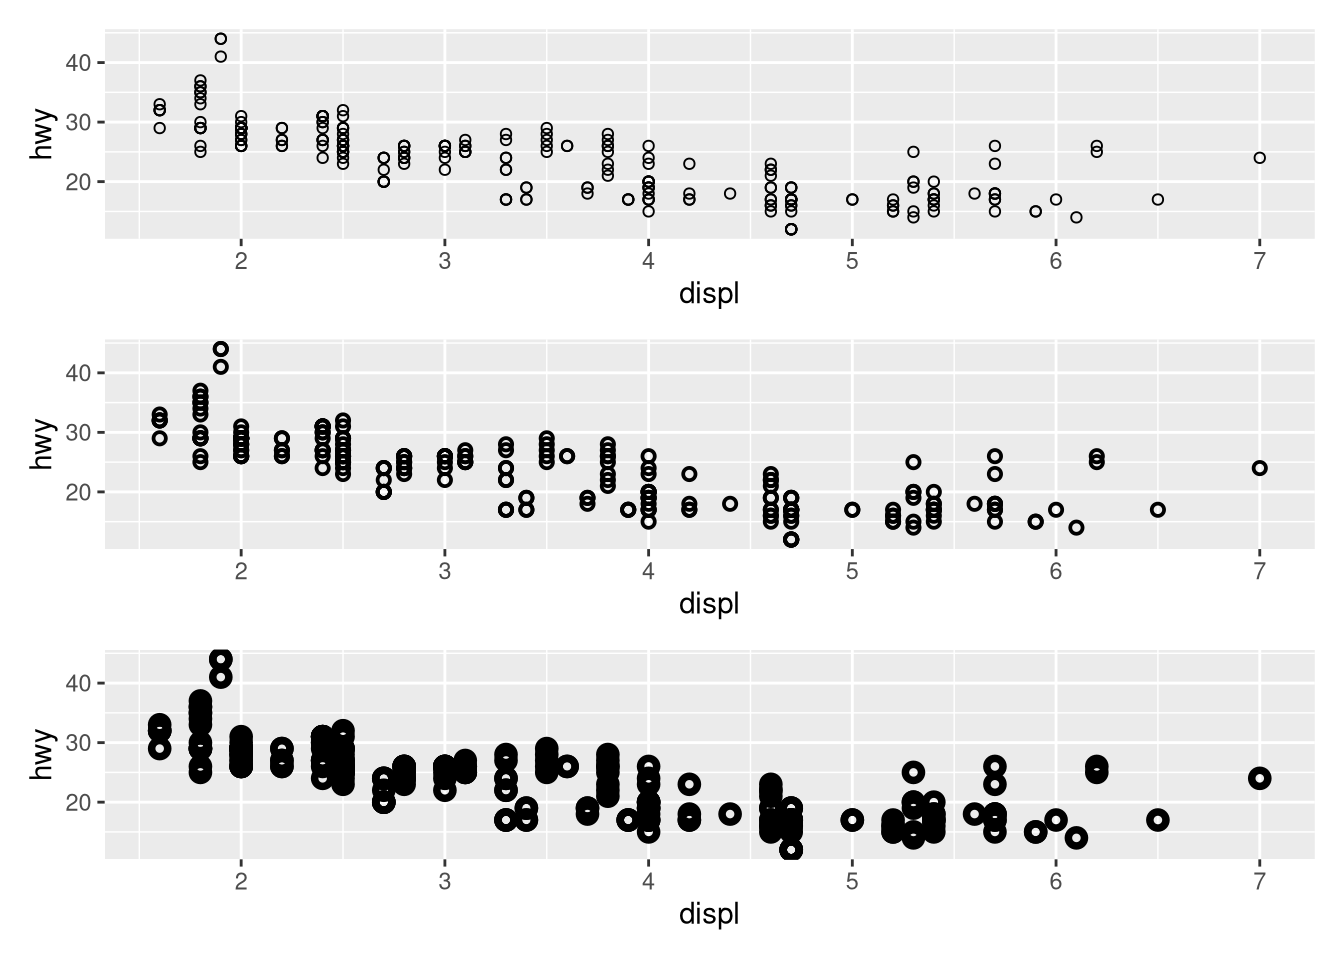
\includegraphics{CH09_files/figure-pdf/unnamed-chunk-5-1.pdf}

  }

  \end{figure}

  \emph{Your text answer here.}

  \end{tcolorbox}
\item
  What happens if you map an aesthetic to something other than a
  variable name, like \texttt{aes(color\ =\ displ\ \textless{}\ 5)}?
  Note, you'll also need to specify x and y.

  \begin{tcolorbox}[enhanced jigsaw, breakable, bottomtitle=1mm, left=2mm, colback=white, toprule=.15mm, leftrule=.75mm, colframe=quarto-callout-note-color-frame, colbacktitle=quarto-callout-note-color!10!white, title={Answer}, coltitle=black, toptitle=1mm, bottomrule=.15mm, opacitybacktitle=0.6, arc=.35mm, rightrule=.15mm, titlerule=0mm, opacityback=0]

\begin{Shaded}
\begin{Highlighting}[]
\NormalTok{mpg }\SpecialCharTok{|\textgreater{}}
  \FunctionTok{ggplot}\NormalTok{(}\FunctionTok{aes}\NormalTok{(}\AttributeTok{x =}\NormalTok{ displ, }\AttributeTok{y =}\NormalTok{ hwy, }\AttributeTok{color =}\NormalTok{ displ }\SpecialCharTok{\textless{}} \DecValTok{5}\NormalTok{)) }\SpecialCharTok{+}
    \FunctionTok{geom\_point}\NormalTok{()}
\end{Highlighting}
\end{Shaded}

  \begin{figure}[H]

  {\centering 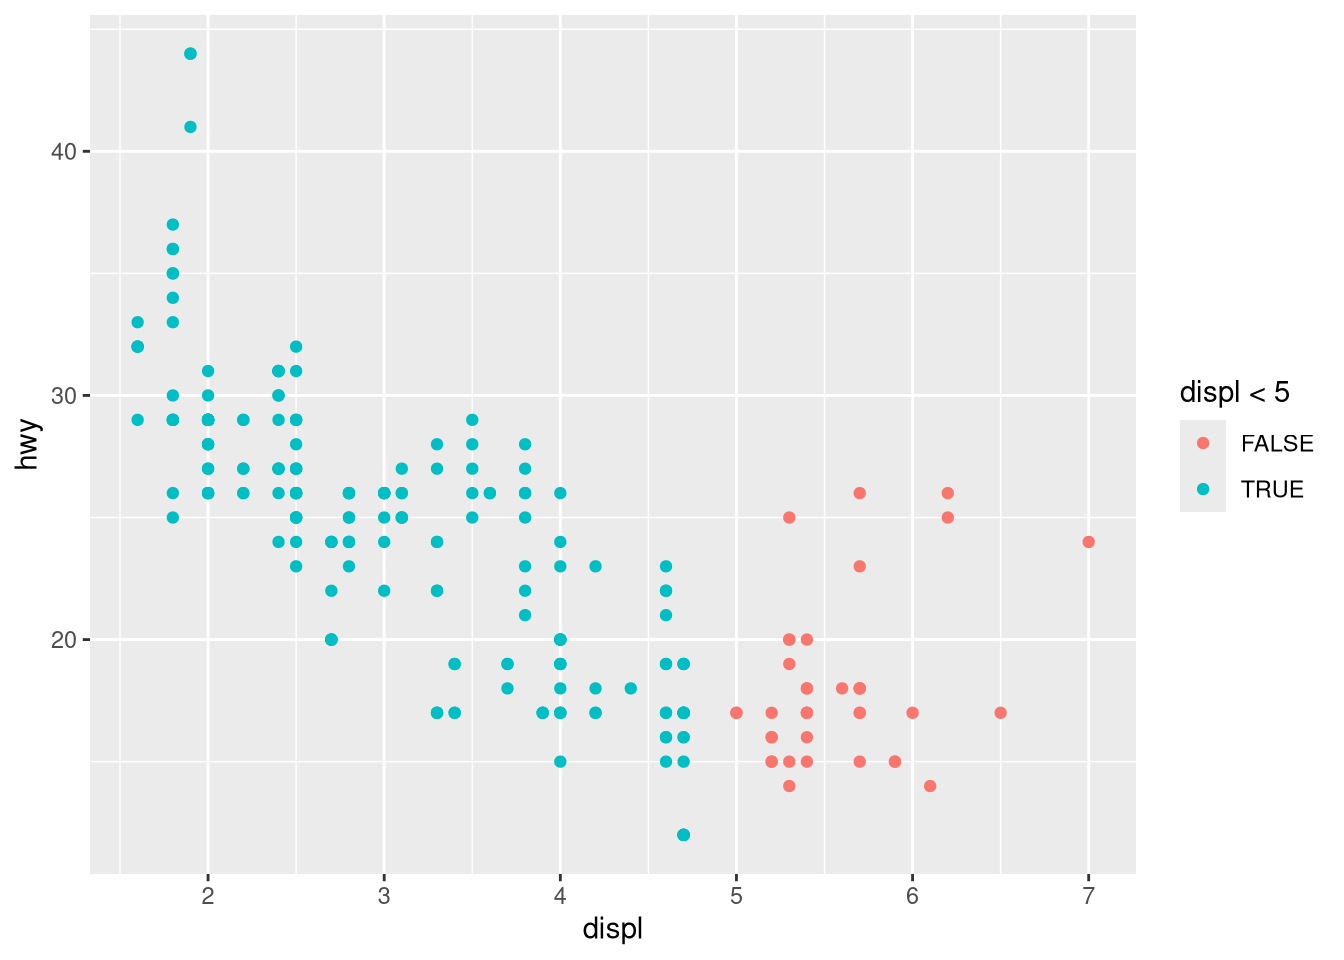
\includegraphics{CH09_files/figure-pdf/unnamed-chunk-6-1.pdf}

  }

  \end{figure}

  \emph{Your text answer here.}

  \end{tcolorbox}
\item
  What geom would you use to draw a line chart? A boxplot? A histogram?
  An area chart?

  \begin{tcolorbox}[enhanced jigsaw, breakable, bottomtitle=1mm, left=2mm, colback=white, toprule=.15mm, leftrule=.75mm, colframe=quarto-callout-note-color-frame, colbacktitle=quarto-callout-note-color!10!white, title={Answer}, coltitle=black, toptitle=1mm, bottomrule=.15mm, opacitybacktitle=0.6, arc=.35mm, rightrule=.15mm, titlerule=0mm, opacityback=0]

  \emph{Your text answer here.}

\begin{Shaded}
\begin{Highlighting}[]
\CommentTok{\# R Code here}
\end{Highlighting}
\end{Shaded}

  \end{tcolorbox}

  \begin{tcolorbox}[enhanced jigsaw, breakable, bottomtitle=1mm, left=2mm, colback=white, toprule=.15mm, leftrule=.75mm, colframe=quarto-callout-note-color-frame, colbacktitle=quarto-callout-note-color!10!white, title={Answer}, coltitle=black, toptitle=1mm, bottomrule=.15mm, opacitybacktitle=0.6, arc=.35mm, rightrule=.15mm, titlerule=0mm, opacityback=0]

  \emph{Your text answer here.}

\begin{Shaded}
\begin{Highlighting}[]
\CommentTok{\# R code here}
\end{Highlighting}
\end{Shaded}

  \end{tcolorbox}

  \begin{tcolorbox}[enhanced jigsaw, breakable, bottomtitle=1mm, left=2mm, colback=white, toprule=.15mm, leftrule=.75mm, colframe=quarto-callout-note-color-frame, colbacktitle=quarto-callout-note-color!10!white, title={Answer}, coltitle=black, toptitle=1mm, bottomrule=.15mm, opacitybacktitle=0.6, arc=.35mm, rightrule=.15mm, titlerule=0mm, opacityback=0]

  \emph{Your text answer here.}

\begin{Shaded}
\begin{Highlighting}[]
\CommentTok{\# R code here}
\end{Highlighting}
\end{Shaded}

  \end{tcolorbox}

  \begin{tcolorbox}[enhanced jigsaw, breakable, bottomtitle=1mm, left=2mm, colback=white, toprule=.15mm, leftrule=.75mm, colframe=quarto-callout-note-color-frame, colbacktitle=quarto-callout-note-color!10!white, title={Answer}, coltitle=black, toptitle=1mm, bottomrule=.15mm, opacitybacktitle=0.6, arc=.35mm, rightrule=.15mm, titlerule=0mm, opacityback=0]

  \emph{Your text answer here.}

\begin{Shaded}
\begin{Highlighting}[]
\CommentTok{\# Youe R code here}
\end{Highlighting}
\end{Shaded}

  \end{tcolorbox}
\item
  Earlier in this chapter we used \texttt{show.legend} without
  explaining it:

\begin{Shaded}
\begin{Highlighting}[]
\FunctionTok{ggplot}\NormalTok{(mpg, }\FunctionTok{aes}\NormalTok{(}\AttributeTok{x =}\NormalTok{ displ, }\AttributeTok{y =}\NormalTok{ hwy)) }\SpecialCharTok{+}
  \FunctionTok{geom\_smooth}\NormalTok{(}\FunctionTok{aes}\NormalTok{(}\AttributeTok{color =}\NormalTok{ drv), }\AttributeTok{show.legend =} \ConstantTok{FALSE}\NormalTok{)}
\end{Highlighting}
\end{Shaded}

  What does \texttt{show.legend\ =\ FALSE} do here? What happens if you
  remove it? Why do you think we used it earlier?

  \begin{tcolorbox}[enhanced jigsaw, breakable, bottomtitle=1mm, left=2mm, colback=white, toprule=.15mm, leftrule=.75mm, colframe=quarto-callout-note-color-frame, colbacktitle=quarto-callout-note-color!10!white, title={Answer}, coltitle=black, toptitle=1mm, bottomrule=.15mm, opacitybacktitle=0.6, arc=.35mm, rightrule=.15mm, titlerule=0mm, opacityback=0]

  \emph{Your text answer here.}

\begin{Shaded}
\begin{Highlighting}[]
\FunctionTok{ggplot}\NormalTok{(mpg, }\FunctionTok{aes}\NormalTok{(}\AttributeTok{x =}\NormalTok{ displ, }\AttributeTok{y =}\NormalTok{ hwy)) }\SpecialCharTok{+}
  \FunctionTok{geom\_smooth}\NormalTok{(}\FunctionTok{aes}\NormalTok{(}\AttributeTok{color =}\NormalTok{ drv), }\AttributeTok{show.legend =} \ConstantTok{FALSE}\NormalTok{) }\OtherTok{{-}\textgreater{}}\NormalTok{ p1}
\FunctionTok{ggplot}\NormalTok{(mpg, }\FunctionTok{aes}\NormalTok{(}\AttributeTok{x =}\NormalTok{ displ, }\AttributeTok{y =}\NormalTok{ hwy)) }\SpecialCharTok{+}
  \FunctionTok{geom\_smooth}\NormalTok{(}\FunctionTok{aes}\NormalTok{(}\AttributeTok{color =}\NormalTok{ drv), }\AttributeTok{show.legend =} \ConstantTok{TRUE}\NormalTok{) }\OtherTok{{-}\textgreater{}}\NormalTok{ p2}
\NormalTok{p1 }\SpecialCharTok{/}\NormalTok{ p2}
\end{Highlighting}
\end{Shaded}

  \begin{figure}[H]

  {\centering \includegraphics{CH09_files/figure-pdf/unnamed-chunk-12-1.pdf}

  }

  \end{figure}

  \end{tcolorbox}
\item
  What does the \texttt{se} argument to \texttt{geom\_smooth()} do?

  \begin{tcolorbox}[enhanced jigsaw, breakable, bottomtitle=1mm, left=2mm, colback=white, toprule=.15mm, leftrule=.75mm, colframe=quarto-callout-note-color-frame, colbacktitle=quarto-callout-note-color!10!white, title={Answer}, coltitle=black, toptitle=1mm, bottomrule=.15mm, opacitybacktitle=0.6, arc=.35mm, rightrule=.15mm, titlerule=0mm, opacityback=0]

  \emph{Your text answer here.}

\begin{Shaded}
\begin{Highlighting}[]
\FunctionTok{ggplot}\NormalTok{(mpg, }\FunctionTok{aes}\NormalTok{(}\AttributeTok{x =}\NormalTok{ displ, }\AttributeTok{y =}\NormalTok{ hwy, }\AttributeTok{color =}\NormalTok{ drv)) }\SpecialCharTok{+}
  \FunctionTok{geom\_smooth}\NormalTok{(}\AttributeTok{se =} \ConstantTok{FALSE}\NormalTok{)}
\end{Highlighting}
\end{Shaded}

  \begin{figure}[H]

  {\centering 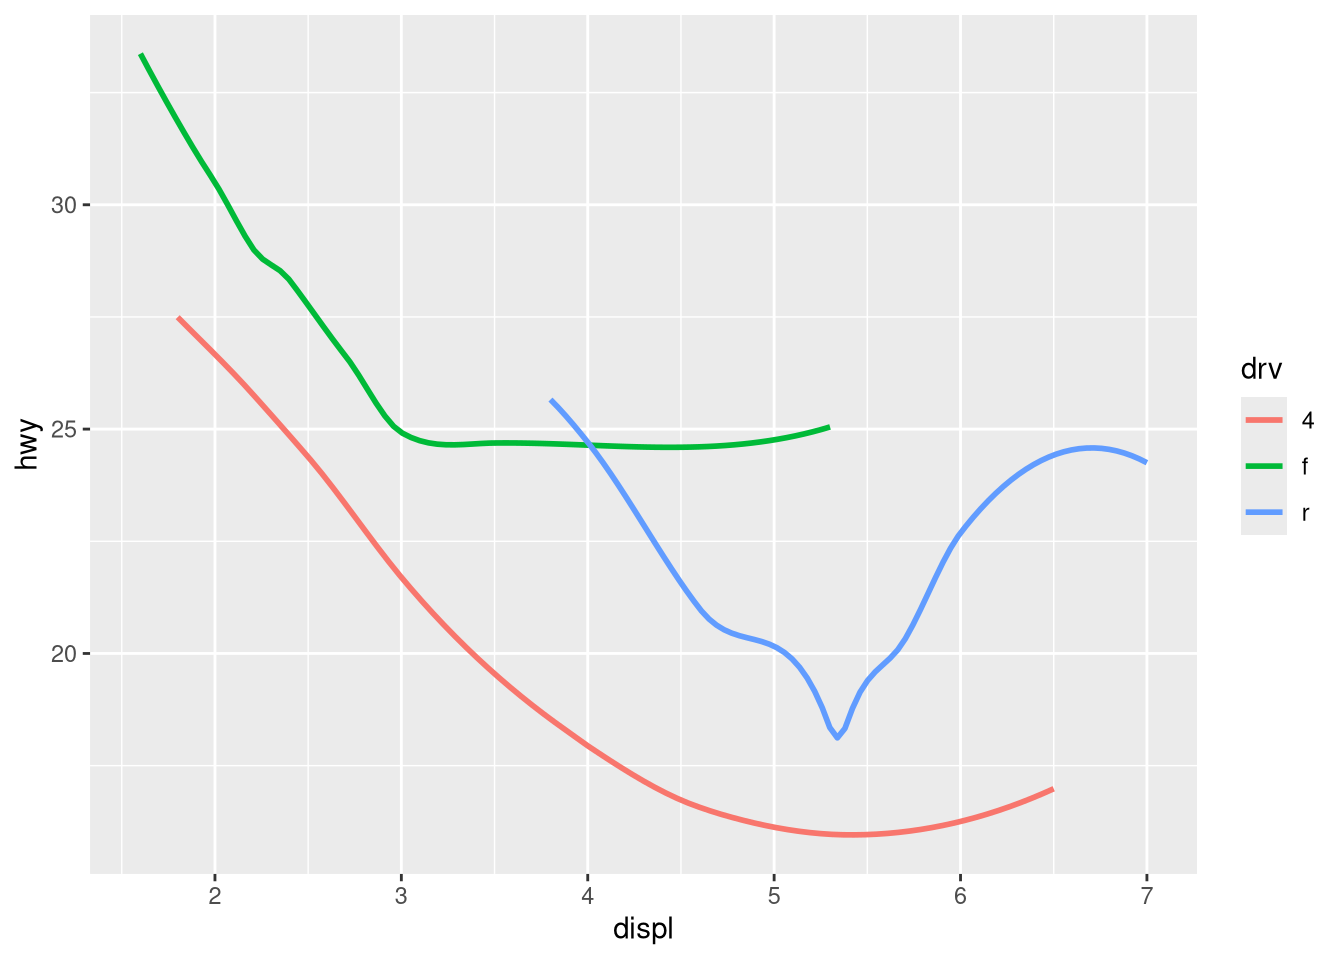
\includegraphics{CH09_files/figure-pdf/unnamed-chunk-13-1.pdf}

  }

  \end{figure}

  \end{tcolorbox}
\item
  Recreate the R code necessary to generate the following graphs. Note
  that wherever a categorical variable is used in the plot, it's
  \texttt{drv}.

  \begin{figure}

  \begin{minipage}[t]{0.50\linewidth}

  {\centering 

  \raisebox{-\height}{

  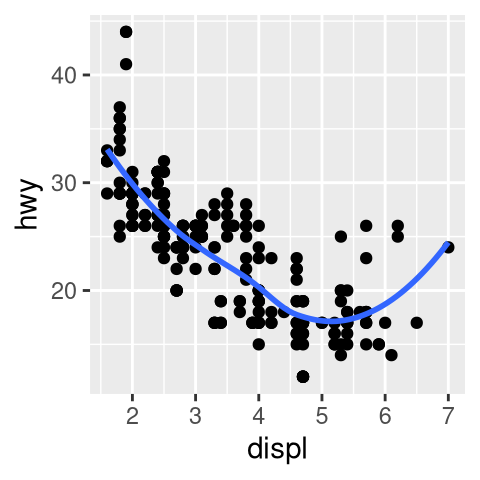
\includegraphics{CH09_files/figure-pdf/unnamed-chunk-14-1.pdf}

  }

  }

  \end{minipage}%
  %
  \begin{minipage}[t]{0.50\linewidth}

  {\centering 

  \raisebox{-\height}{

  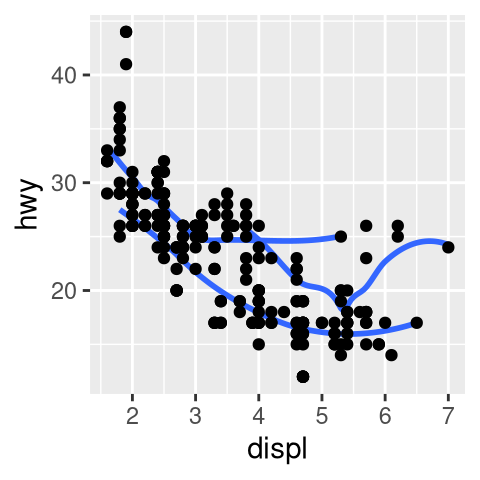
\includegraphics{CH09_files/figure-pdf/unnamed-chunk-14-2.pdf}

  }

  }

  \end{minipage}%
  \newline
  \begin{minipage}[t]{0.50\linewidth}

  {\centering 

  \raisebox{-\height}{

  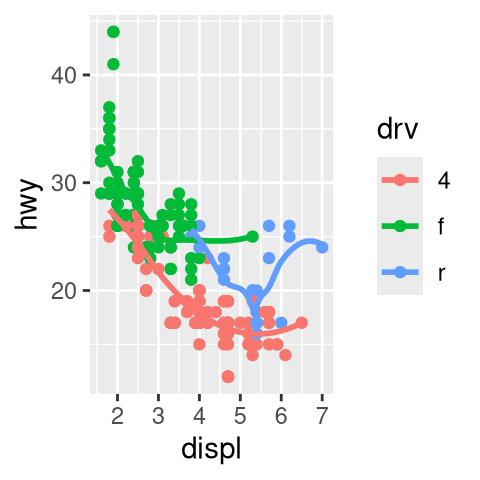
\includegraphics{CH09_files/figure-pdf/unnamed-chunk-14-3.pdf}

  }

  }

  \end{minipage}%
  %
  \begin{minipage}[t]{0.50\linewidth}

  {\centering 

  \raisebox{-\height}{

  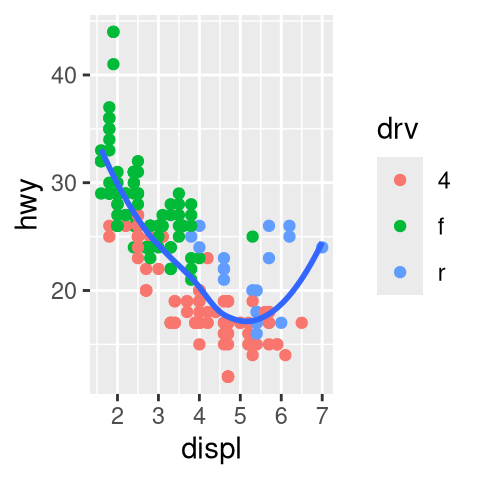
\includegraphics{CH09_files/figure-pdf/unnamed-chunk-14-4.pdf}

  }

  }

  \end{minipage}%
  \newline
  \begin{minipage}[t]{0.50\linewidth}

  {\centering 

  \raisebox{-\height}{

  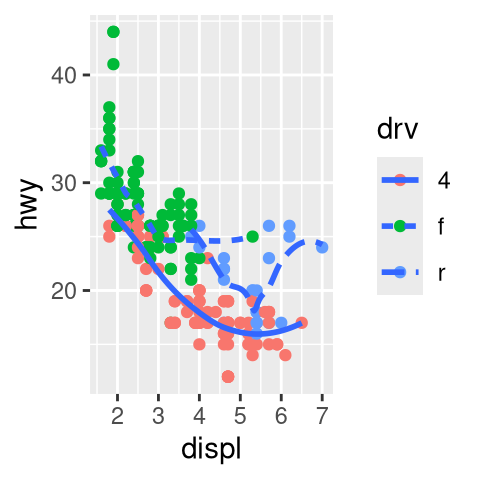
\includegraphics{CH09_files/figure-pdf/unnamed-chunk-14-5.pdf}

  }

  }

  \end{minipage}%
  %
  \begin{minipage}[t]{0.50\linewidth}

  {\centering 

  \raisebox{-\height}{

  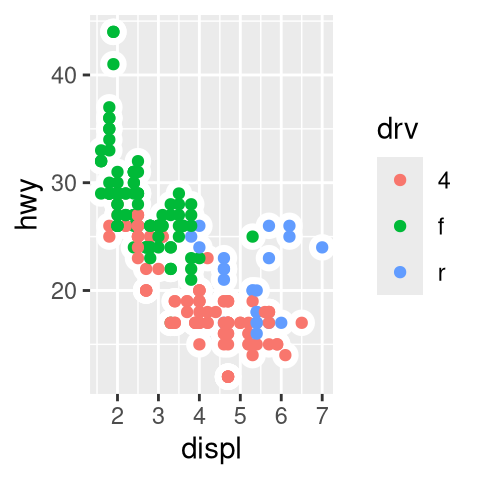
\includegraphics{CH09_files/figure-pdf/unnamed-chunk-14-6.pdf}

  }

  }

  \end{minipage}%

  \end{figure}

  \begin{tcolorbox}[enhanced jigsaw, breakable, bottomtitle=1mm, left=2mm, colback=white, toprule=.15mm, leftrule=.75mm, colframe=quarto-callout-note-color-frame, colbacktitle=quarto-callout-note-color!10!white, title={Answer}, coltitle=black, toptitle=1mm, bottomrule=.15mm, opacitybacktitle=0.6, arc=.35mm, rightrule=.15mm, titlerule=0mm, opacityback=0]

  The code for each of the plots is given below.

\begin{Shaded}
\begin{Highlighting}[]
\CommentTok{\# Your R code here}
\end{Highlighting}
\end{Shaded}

  \end{tcolorbox}
\item
  What happens if you facet on a continuous variable?

  \begin{tcolorbox}[enhanced jigsaw, breakable, bottomtitle=1mm, left=2mm, colback=white, toprule=.15mm, leftrule=.75mm, colframe=quarto-callout-note-color-frame, colbacktitle=quarto-callout-note-color!10!white, title={Answer}, coltitle=black, toptitle=1mm, bottomrule=.15mm, opacitybacktitle=0.6, arc=.35mm, rightrule=.15mm, titlerule=0mm, opacityback=0]

  \emph{Your text answer here.}

\begin{Shaded}
\begin{Highlighting}[]
\NormalTok{mpg }\SpecialCharTok{|\textgreater{}} 
  \FunctionTok{ggplot}\NormalTok{(}\FunctionTok{aes}\NormalTok{(}\AttributeTok{x =}\NormalTok{ drv, }\AttributeTok{y =}\NormalTok{ cyl)) }\SpecialCharTok{+} 
  \FunctionTok{geom\_point}\NormalTok{() }\SpecialCharTok{+} 
  \FunctionTok{facet\_wrap}\NormalTok{(}\SpecialCharTok{\textasciitilde{}}\NormalTok{hwy)}
\end{Highlighting}
\end{Shaded}

  \begin{figure}[H]

  {\centering 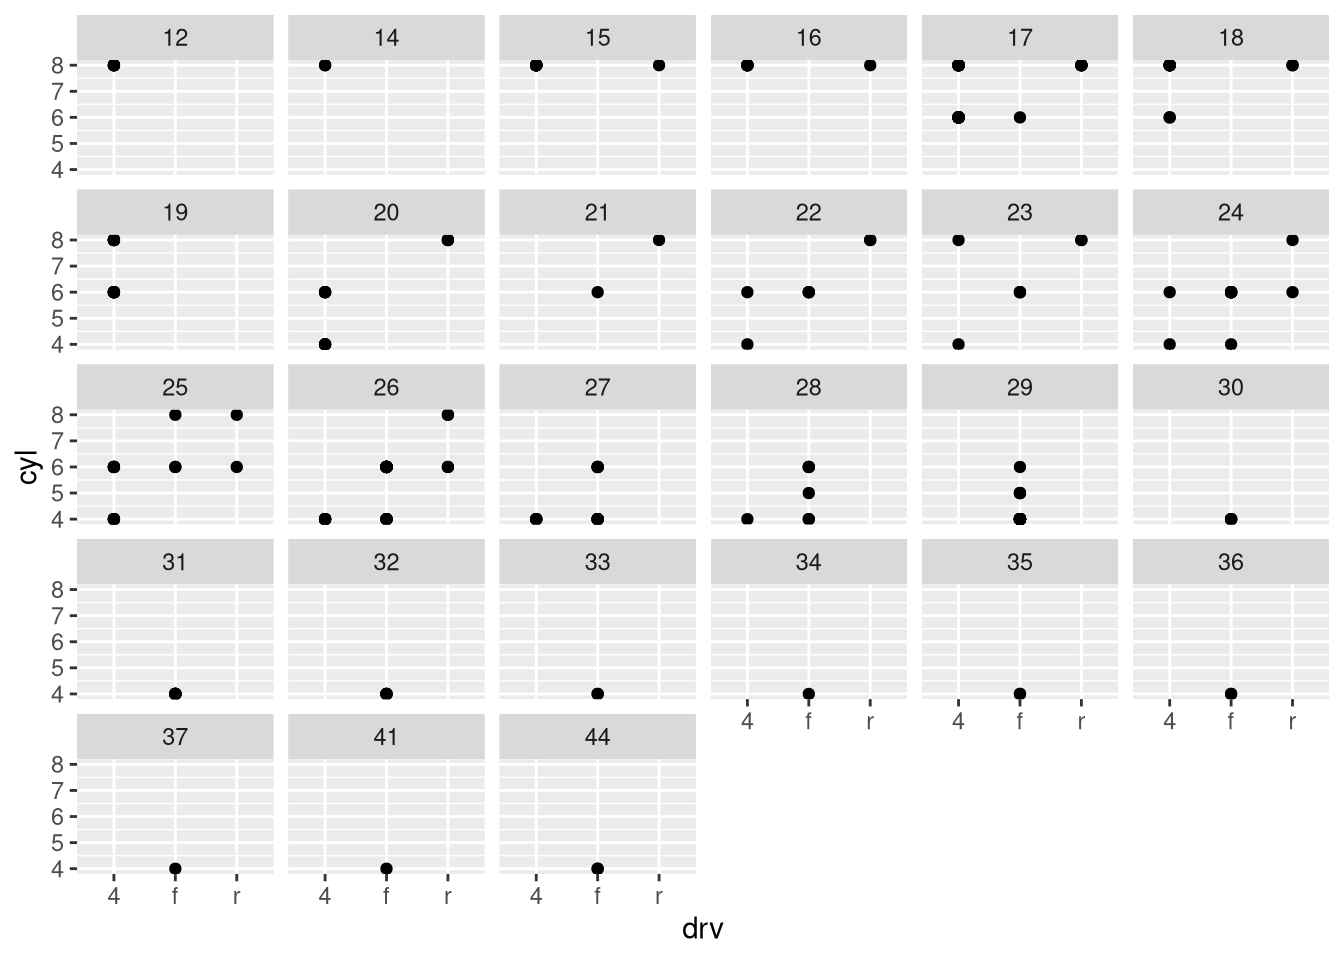
\includegraphics{CH09_files/figure-pdf/unnamed-chunk-16-1.pdf}

  }

  \end{figure}

  \end{tcolorbox}
\item
  What do the empty cells in the plot above with
  \texttt{facet\_grid(drv\ \textasciitilde{}\ cyl)} mean? Run the
  following code. How do they relate to the resulting plot?

\begin{Shaded}
\begin{Highlighting}[]
\FunctionTok{ggplot}\NormalTok{(mpg) }\SpecialCharTok{+} 
  \FunctionTok{geom\_point}\NormalTok{(}\FunctionTok{aes}\NormalTok{(}\AttributeTok{x =}\NormalTok{ drv, }\AttributeTok{y =}\NormalTok{ cyl))}
\end{Highlighting}
\end{Shaded}

  \begin{tcolorbox}[enhanced jigsaw, breakable, bottomtitle=1mm, left=2mm, colback=white, toprule=.15mm, leftrule=.75mm, colframe=quarto-callout-note-color-frame, colbacktitle=quarto-callout-note-color!10!white, title={Answer}, coltitle=black, toptitle=1mm, bottomrule=.15mm, opacitybacktitle=0.6, arc=.35mm, rightrule=.15mm, titlerule=0mm, opacityback=0]

\begin{Shaded}
\begin{Highlighting}[]
\FunctionTok{ggplot}\NormalTok{(mpg) }\SpecialCharTok{+} 
  \FunctionTok{geom\_point}\NormalTok{(}\FunctionTok{aes}\NormalTok{(}\AttributeTok{x =}\NormalTok{ drv, }\AttributeTok{y =}\NormalTok{ cyl)) }\SpecialCharTok{+}
  \FunctionTok{facet\_grid}\NormalTok{(drv }\SpecialCharTok{\textasciitilde{}}\NormalTok{ cyl)}
\end{Highlighting}
\end{Shaded}

  \begin{figure}[H]

  {\centering 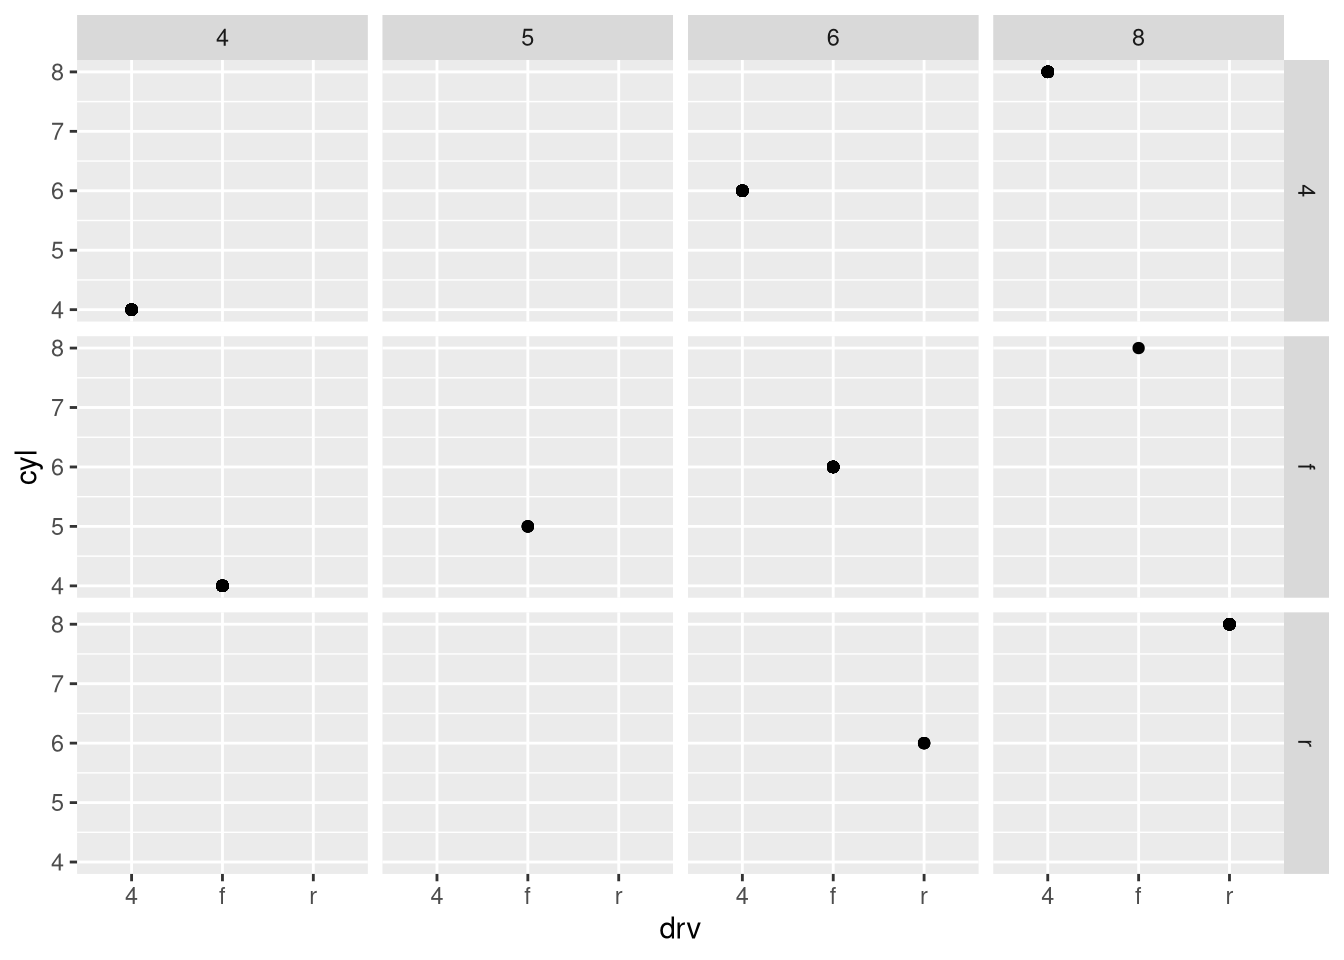
\includegraphics{CH09_files/figure-pdf/unnamed-chunk-18-1.pdf}

  }

  \end{figure}

  \emph{Your text answer here.}

  \end{tcolorbox}
\item
  What plots does the following code make? What does \texttt{.} do?

\begin{Shaded}
\begin{Highlighting}[]
\FunctionTok{ggplot}\NormalTok{(mpg) }\SpecialCharTok{+} 
  \FunctionTok{geom\_point}\NormalTok{(}\FunctionTok{aes}\NormalTok{(}\AttributeTok{x =}\NormalTok{ displ, }\AttributeTok{y =}\NormalTok{ hwy)) }\SpecialCharTok{+}
  \FunctionTok{facet\_grid}\NormalTok{(drv }\SpecialCharTok{\textasciitilde{}}\NormalTok{ .)}
\end{Highlighting}
\end{Shaded}

\begin{Shaded}
\begin{Highlighting}[]
\FunctionTok{ggplot}\NormalTok{(mpg) }\SpecialCharTok{+} 
  \FunctionTok{geom\_point}\NormalTok{(}\FunctionTok{aes}\NormalTok{(}\AttributeTok{x =}\NormalTok{ displ, }\AttributeTok{y =}\NormalTok{ hwy)) }\SpecialCharTok{+}
  \FunctionTok{facet\_grid}\NormalTok{(. }\SpecialCharTok{\textasciitilde{}}\NormalTok{ cyl)}
\end{Highlighting}
\end{Shaded}

  \begin{tcolorbox}[enhanced jigsaw, breakable, bottomtitle=1mm, left=2mm, colback=white, toprule=.15mm, leftrule=.75mm, colframe=quarto-callout-note-color-frame, colbacktitle=quarto-callout-note-color!10!white, title={Answer}, coltitle=black, toptitle=1mm, bottomrule=.15mm, opacitybacktitle=0.6, arc=.35mm, rightrule=.15mm, titlerule=0mm, opacityback=0]

\begin{Shaded}
\begin{Highlighting}[]
\FunctionTok{ggplot}\NormalTok{(mpg) }\SpecialCharTok{+} 
  \FunctionTok{geom\_point}\NormalTok{(}\FunctionTok{aes}\NormalTok{(}\AttributeTok{x =}\NormalTok{ displ, }\AttributeTok{y =}\NormalTok{ hwy)) }\SpecialCharTok{+}
  \FunctionTok{facet\_grid}\NormalTok{(drv }\SpecialCharTok{\textasciitilde{}}\NormalTok{ .)}
\end{Highlighting}
\end{Shaded}

  \begin{figure}[H]

  {\centering 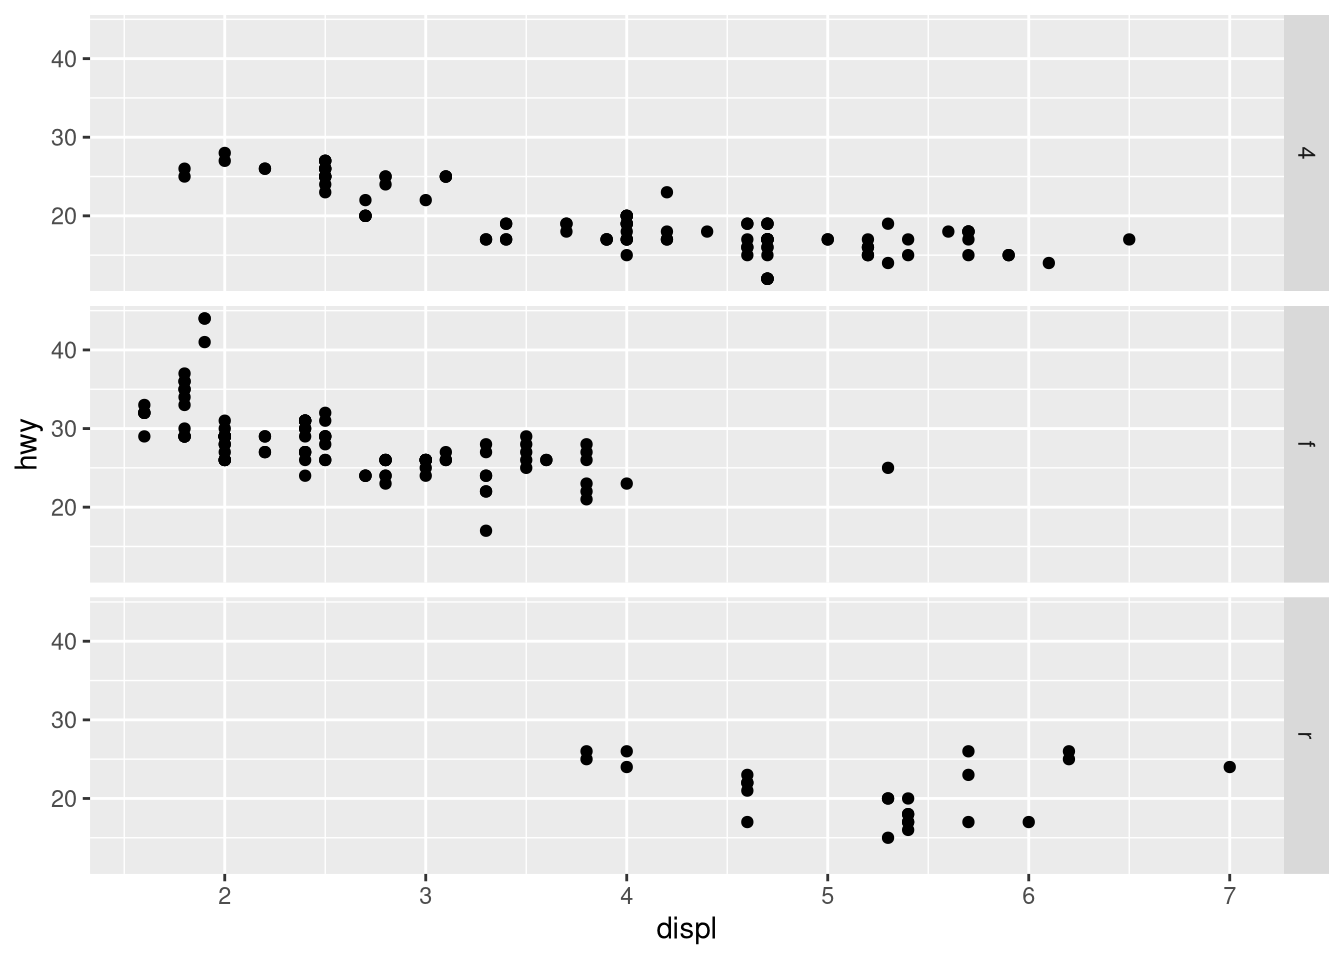
\includegraphics{CH09_files/figure-pdf/unnamed-chunk-20-1.pdf}

  }

  \end{figure}

  \emph{Your text answer here.}

\begin{Shaded}
\begin{Highlighting}[]
\FunctionTok{ggplot}\NormalTok{(mpg) }\SpecialCharTok{+} 
  \FunctionTok{geom\_point}\NormalTok{(}\FunctionTok{aes}\NormalTok{(}\AttributeTok{x =}\NormalTok{ displ, }\AttributeTok{y =}\NormalTok{ hwy)) }\SpecialCharTok{+}
  \FunctionTok{facet\_grid}\NormalTok{(. }\SpecialCharTok{\textasciitilde{}}\NormalTok{ cyl)}
\end{Highlighting}
\end{Shaded}

  \begin{figure}[H]

  {\centering 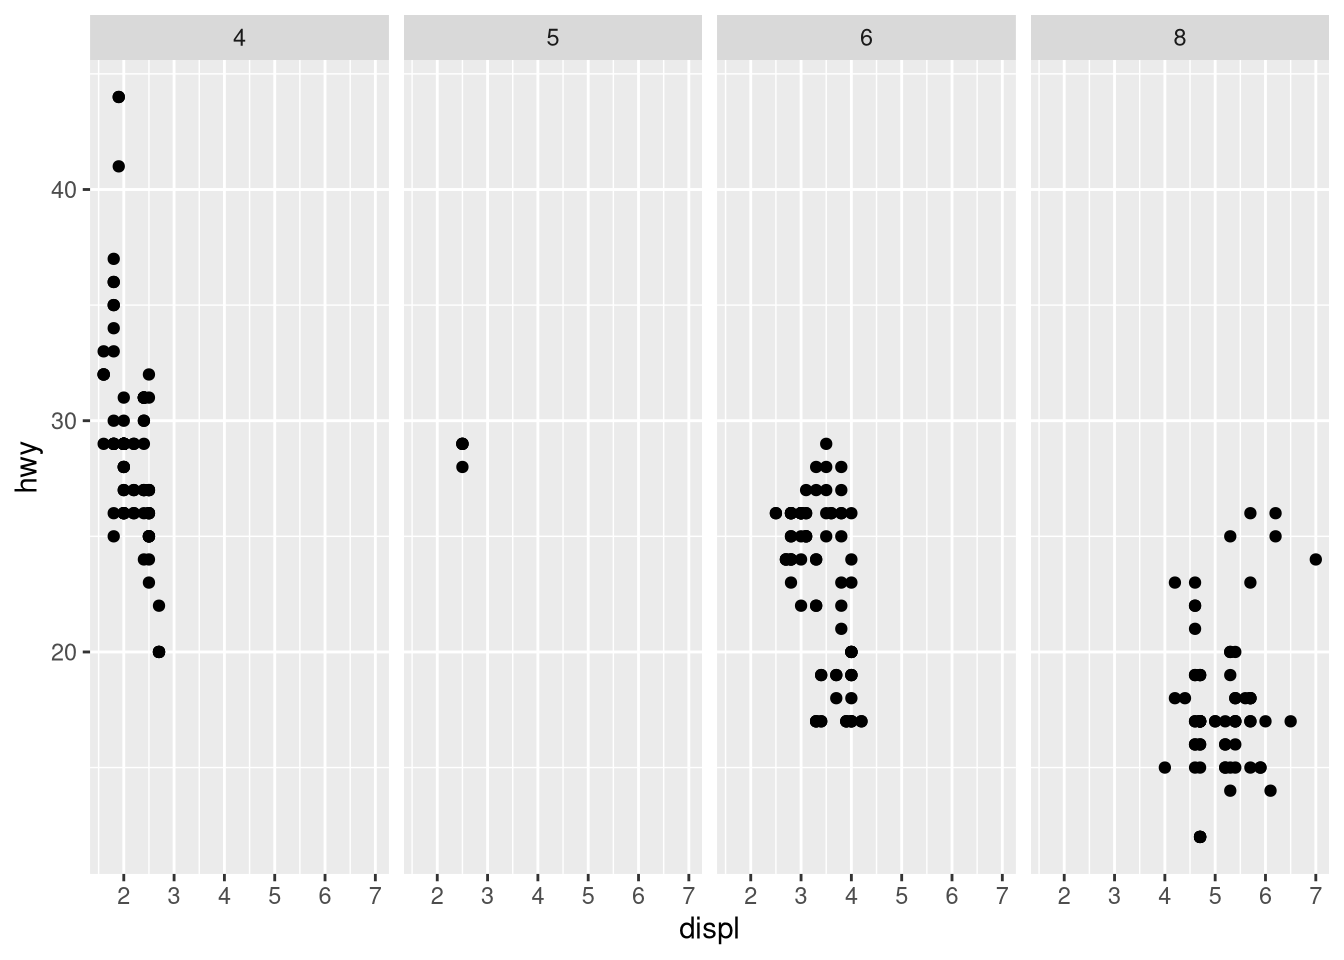
\includegraphics{CH09_files/figure-pdf/unnamed-chunk-21-1.pdf}

  }

  \end{figure}

  \emph{Your text answer here.}

  \end{tcolorbox}
\item
  Take the first faceted plot in this section:

\begin{Shaded}
\begin{Highlighting}[]
\FunctionTok{ggplot}\NormalTok{(mpg) }\SpecialCharTok{+} 
  \FunctionTok{geom\_point}\NormalTok{(}\FunctionTok{aes}\NormalTok{(}\AttributeTok{x =}\NormalTok{ displ, }\AttributeTok{y =}\NormalTok{ hwy)) }\SpecialCharTok{+} 
  \FunctionTok{facet\_wrap}\NormalTok{(}\SpecialCharTok{\textasciitilde{}}\NormalTok{ cyl, }\AttributeTok{nrow =} \DecValTok{2}\NormalTok{)}
\end{Highlighting}
\end{Shaded}

  What are the advantages to using faceting instead of the color
  aesthetic? What are the disadvantages? How might the balance change if
  you had a larger dataset?

  \begin{tcolorbox}[enhanced jigsaw, breakable, bottomtitle=1mm, left=2mm, colback=white, toprule=.15mm, leftrule=.75mm, colframe=quarto-callout-note-color-frame, colbacktitle=quarto-callout-note-color!10!white, title={Answer}, coltitle=black, toptitle=1mm, bottomrule=.15mm, opacitybacktitle=0.6, arc=.35mm, rightrule=.15mm, titlerule=0mm, opacityback=0]

  \emph{Your text answer here.}

\begin{Shaded}
\begin{Highlighting}[]
\CommentTok{\# facet}
\FunctionTok{ggplot}\NormalTok{(mpg) }\SpecialCharTok{+} 
 \FunctionTok{geom\_point}\NormalTok{(}\FunctionTok{aes}\NormalTok{(}\AttributeTok{x =}\NormalTok{ displ, }\AttributeTok{y =}\NormalTok{ hwy)) }\SpecialCharTok{+} 
  \FunctionTok{facet\_wrap}\NormalTok{(}\SpecialCharTok{\textasciitilde{}}\NormalTok{ class, }\AttributeTok{nrow =} \DecValTok{2}\NormalTok{)}
\end{Highlighting}
\end{Shaded}

  \begin{figure}[H]

  {\centering 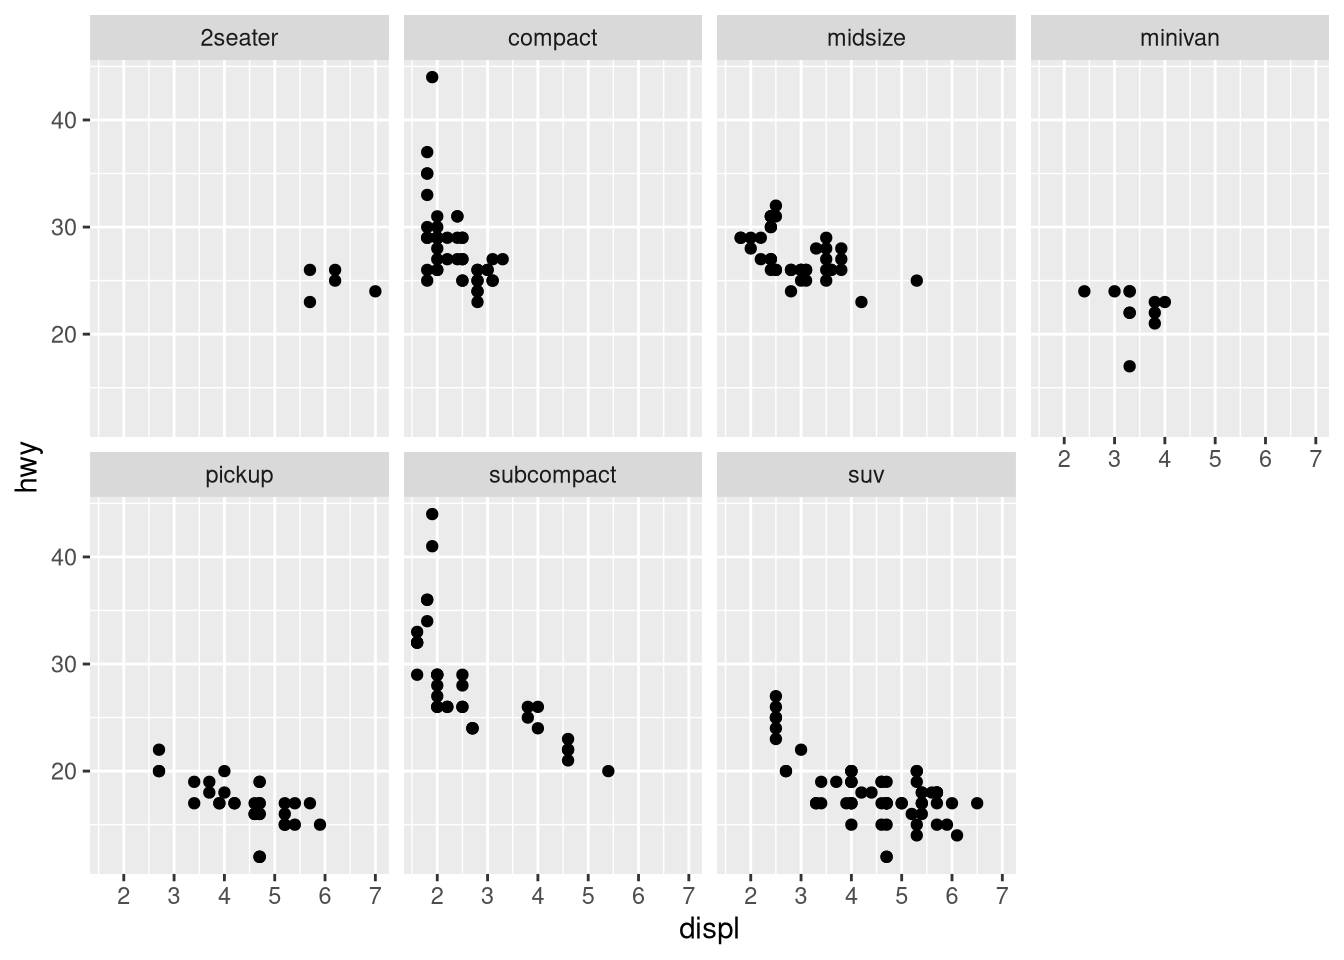
\includegraphics{CH09_files/figure-pdf/unnamed-chunk-23-1.pdf}

  }

  \end{figure}

\begin{Shaded}
\begin{Highlighting}[]
\CommentTok{\# color}
\FunctionTok{ggplot}\NormalTok{(mpg) }\SpecialCharTok{+} 
  \FunctionTok{geom\_point}\NormalTok{(}\FunctionTok{aes}\NormalTok{(}\AttributeTok{x =}\NormalTok{ displ, }\AttributeTok{y =}\NormalTok{ hwy, }\AttributeTok{color =}\NormalTok{ class))}
\end{Highlighting}
\end{Shaded}

  \begin{figure}[H]

  {\centering 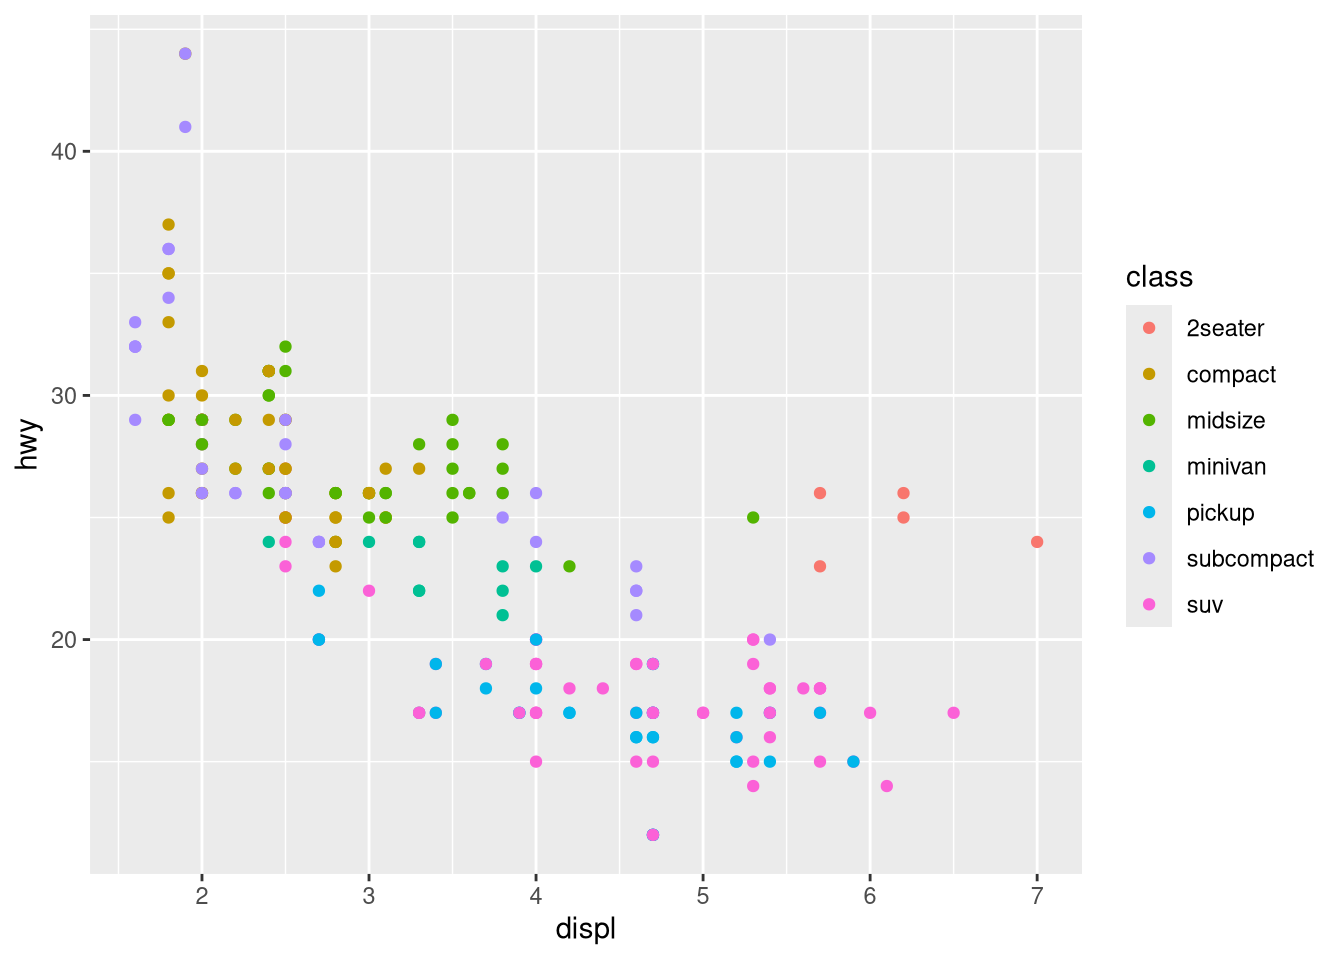
\includegraphics{CH09_files/figure-pdf/unnamed-chunk-23-2.pdf}

  }

  \end{figure}

\begin{Shaded}
\begin{Highlighting}[]
\CommentTok{\# both}
\FunctionTok{ggplot}\NormalTok{(mpg) }\SpecialCharTok{+} 
  \FunctionTok{geom\_point}\NormalTok{(}
    \FunctionTok{aes}\NormalTok{(}\AttributeTok{x =}\NormalTok{ displ, }\AttributeTok{y =}\NormalTok{ hwy, }\AttributeTok{color =}\NormalTok{ class), }
    \AttributeTok{show.legend =} \ConstantTok{FALSE}\NormalTok{) }\SpecialCharTok{+} 
 \FunctionTok{facet\_wrap}\NormalTok{(}\SpecialCharTok{\textasciitilde{}}\NormalTok{ class, }\AttributeTok{nrow =} \DecValTok{2}\NormalTok{)}
\end{Highlighting}
\end{Shaded}

  \begin{figure}[H]

  {\centering 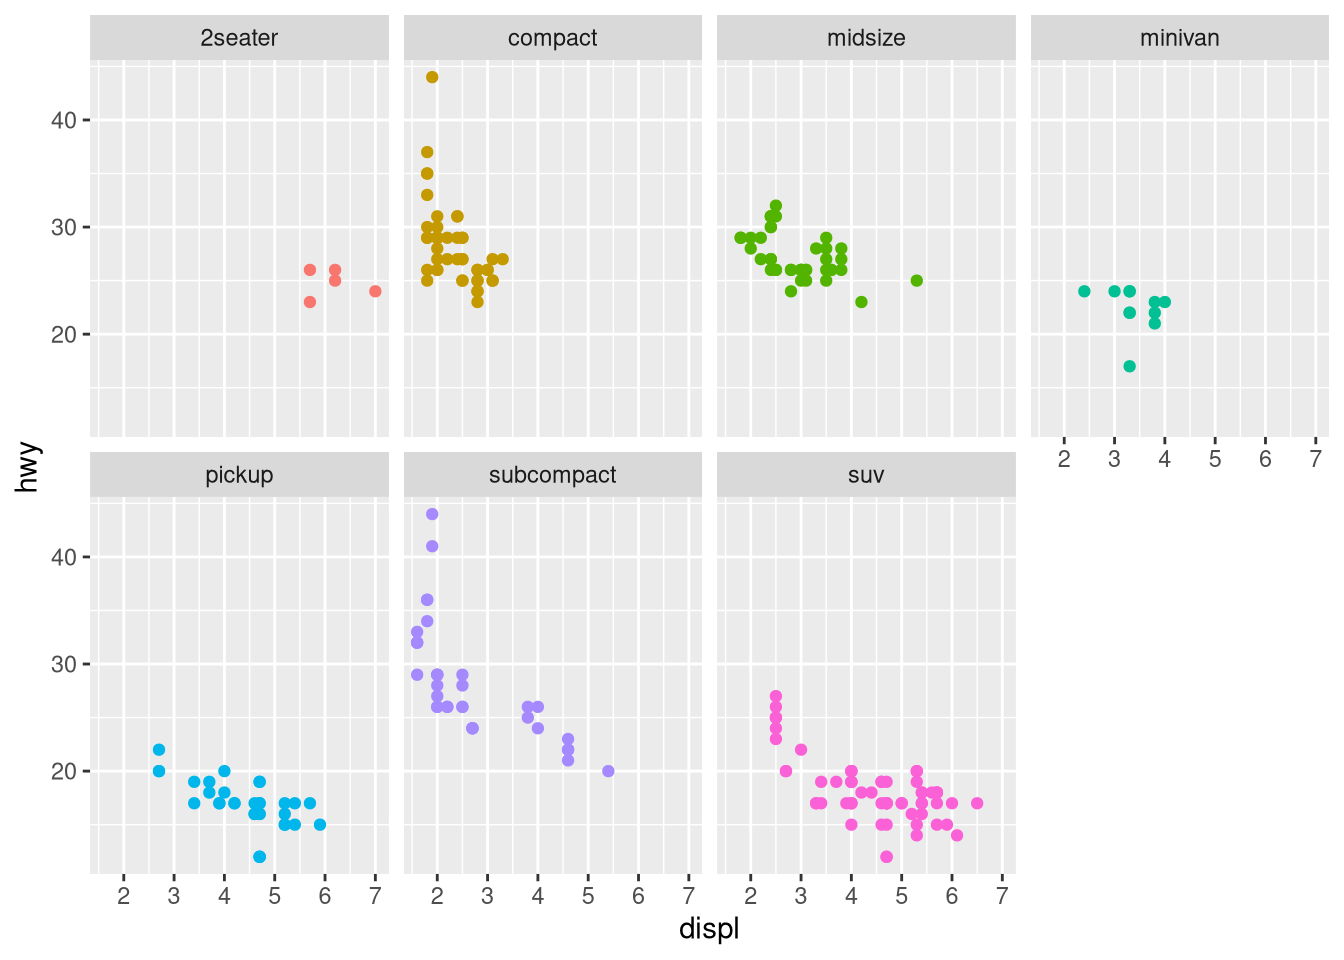
\includegraphics{CH09_files/figure-pdf/unnamed-chunk-23-3.pdf}

  }

  \end{figure}

\begin{Shaded}
\begin{Highlighting}[]
\CommentTok{\# highlighting}
\FunctionTok{ggplot}\NormalTok{(mpg, }\FunctionTok{aes}\NormalTok{(}\AttributeTok{x =}\NormalTok{ displ, }\AttributeTok{y =}\NormalTok{ hwy)) }\SpecialCharTok{+} 
  \FunctionTok{geom\_point}\NormalTok{(}\AttributeTok{color =} \StringTok{"gray"}\NormalTok{) }\SpecialCharTok{+}
  \FunctionTok{geom\_point}\NormalTok{(}
    \AttributeTok{data =}\NormalTok{ mpg }\SpecialCharTok{|\textgreater{}} \FunctionTok{filter}\NormalTok{(class }\SpecialCharTok{==} \StringTok{"compact"}\NormalTok{),}
    \AttributeTok{color =} \StringTok{"pink"}
\NormalTok{  )}
\end{Highlighting}
\end{Shaded}

  \begin{figure}[H]

  {\centering 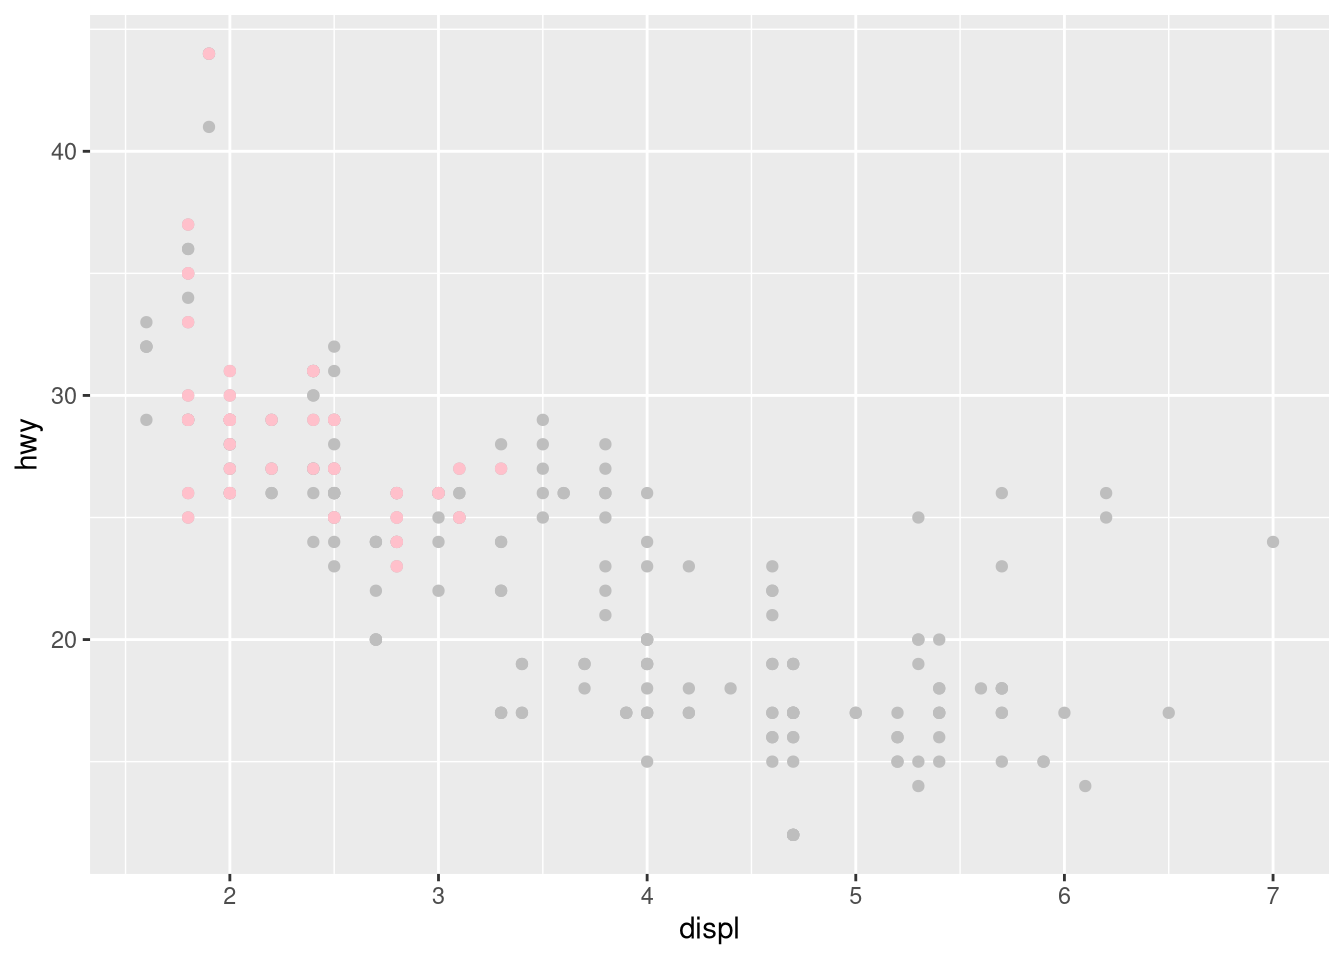
\includegraphics{CH09_files/figure-pdf/unnamed-chunk-23-4.pdf}

  }

  \end{figure}

  \end{tcolorbox}
\item
  Read \texttt{?facet\_wrap}. What does \texttt{nrow} do? What does
  \texttt{ncol} do? What other options control the layout of the
  individual panels? Why doesn't \texttt{facet\_grid()} have
  \texttt{nrow} and \texttt{ncol} arguments?

  \begin{tcolorbox}[enhanced jigsaw, breakable, bottomtitle=1mm, left=2mm, colback=white, toprule=.15mm, leftrule=.75mm, colframe=quarto-callout-note-color-frame, colbacktitle=quarto-callout-note-color!10!white, title={Answer}, coltitle=black, toptitle=1mm, bottomrule=.15mm, opacitybacktitle=0.6, arc=.35mm, rightrule=.15mm, titlerule=0mm, opacityback=0]

  \emph{Your text answer here.}

  \end{tcolorbox}
\item
  Which of the following plots makes it easier to compare engine size
  (\texttt{displ}) across cars with different drive trains? What does
  this say about when to place a faceting variable across rows or
  columns?

\begin{Shaded}
\begin{Highlighting}[]
\FunctionTok{ggplot}\NormalTok{(mpg, }\FunctionTok{aes}\NormalTok{(}\AttributeTok{x =}\NormalTok{ displ)) }\SpecialCharTok{+} 
  \FunctionTok{geom\_histogram}\NormalTok{() }\SpecialCharTok{+} 
  \FunctionTok{facet\_grid}\NormalTok{(drv }\SpecialCharTok{\textasciitilde{}}\NormalTok{ .)}
\end{Highlighting}
\end{Shaded}

\begin{Shaded}
\begin{Highlighting}[]
\FunctionTok{ggplot}\NormalTok{(mpg, }\FunctionTok{aes}\NormalTok{(}\AttributeTok{x =}\NormalTok{ displ)) }\SpecialCharTok{+} 
  \FunctionTok{geom\_histogram}\NormalTok{() }\SpecialCharTok{+}
  \FunctionTok{facet\_grid}\NormalTok{(. }\SpecialCharTok{\textasciitilde{}}\NormalTok{ drv)}
\end{Highlighting}
\end{Shaded}

  \begin{tcolorbox}[enhanced jigsaw, breakable, bottomtitle=1mm, left=2mm, colback=white, toprule=.15mm, leftrule=.75mm, colframe=quarto-callout-note-color-frame, colbacktitle=quarto-callout-note-color!10!white, title={Answer}, coltitle=black, toptitle=1mm, bottomrule=.15mm, opacitybacktitle=0.6, arc=.35mm, rightrule=.15mm, titlerule=0mm, opacityback=0]

\begin{Shaded}
\begin{Highlighting}[]
\FunctionTok{ggplot}\NormalTok{(mpg, }\FunctionTok{aes}\NormalTok{(}\AttributeTok{x =}\NormalTok{ displ)) }\SpecialCharTok{+} 
  \FunctionTok{geom\_histogram}\NormalTok{() }\SpecialCharTok{+} 
  \FunctionTok{facet\_grid}\NormalTok{(drv }\SpecialCharTok{\textasciitilde{}}\NormalTok{ .)}
\end{Highlighting}
\end{Shaded}

\begin{verbatim}
`stat_bin()` using `bins = 30`. Pick better value with `binwidth`.
\end{verbatim}

  \begin{figure}[H]

  {\centering 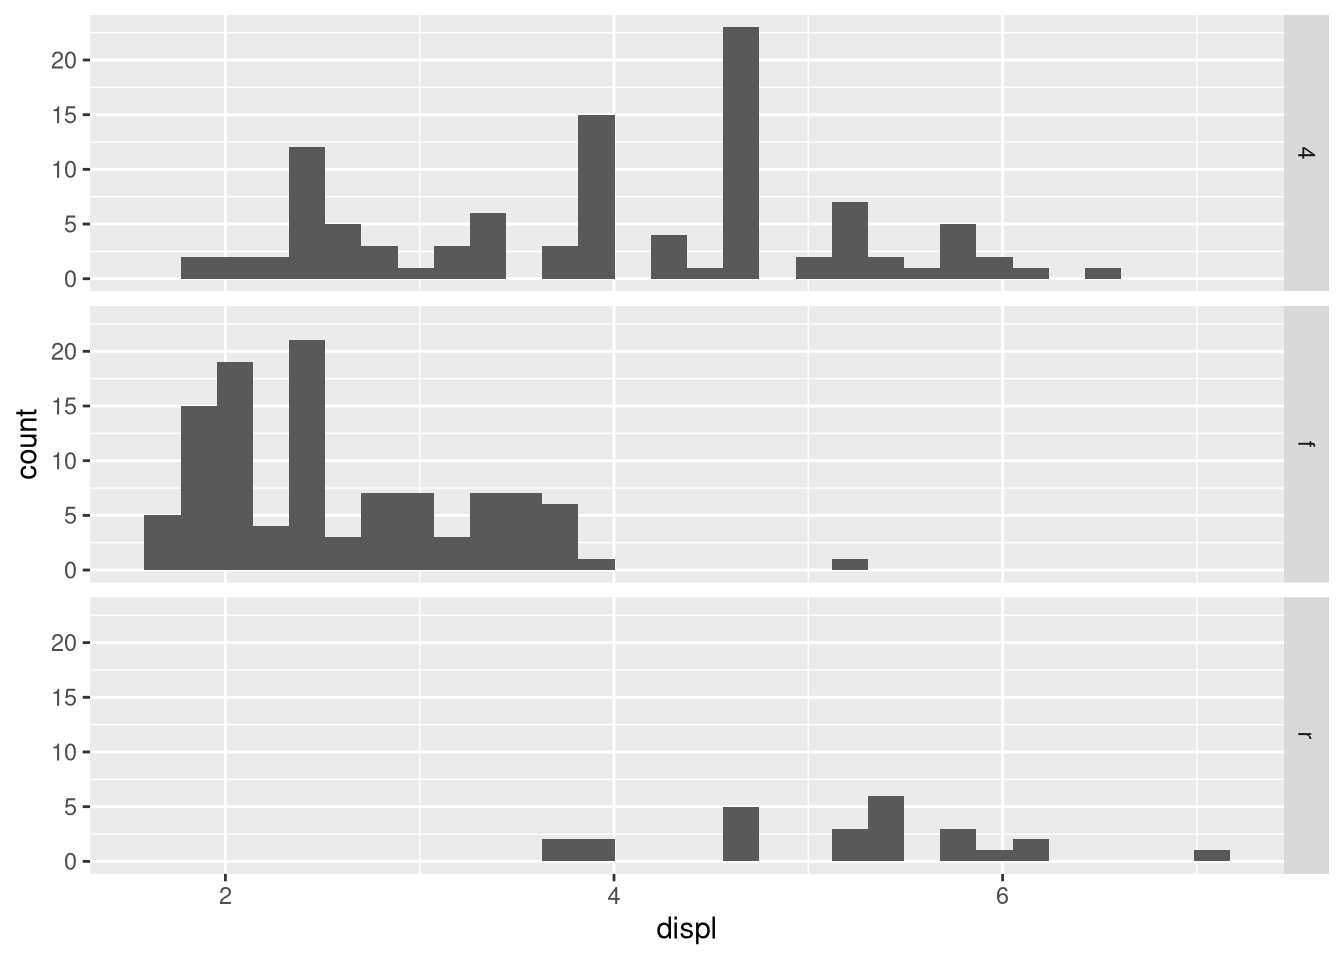
\includegraphics{CH09_files/figure-pdf/unnamed-chunk-25-1.pdf}

  }

  \end{figure}

\begin{Shaded}
\begin{Highlighting}[]
\FunctionTok{ggplot}\NormalTok{(mpg, }\FunctionTok{aes}\NormalTok{(}\AttributeTok{x =}\NormalTok{ displ)) }\SpecialCharTok{+} 
  \FunctionTok{geom\_histogram}\NormalTok{() }\SpecialCharTok{+}
  \FunctionTok{facet\_grid}\NormalTok{(. }\SpecialCharTok{\textasciitilde{}}\NormalTok{ drv)}
\end{Highlighting}
\end{Shaded}

\begin{verbatim}
`stat_bin()` using `bins = 30`. Pick better value with `binwidth`.
\end{verbatim}

  \begin{figure}[H]

  {\centering 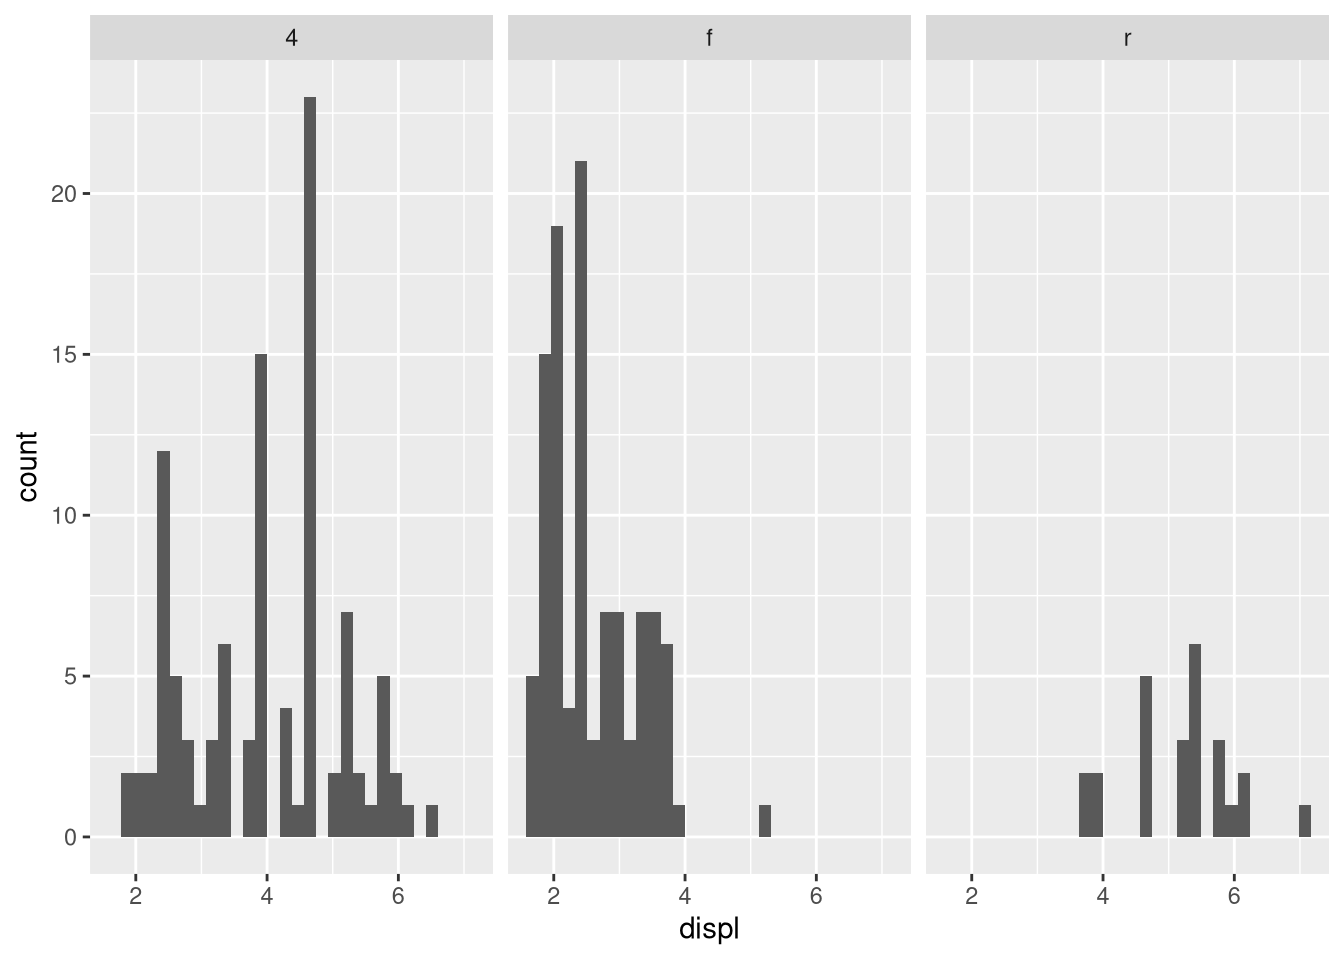
\includegraphics{CH09_files/figure-pdf/unnamed-chunk-25-2.pdf}

  }

  \end{figure}

  \emph{Your text answer here.}

  \end{tcolorbox}
\item
  Recreate the following plot using \texttt{facet\_wrap()} instead of
  \texttt{facet\_grid()}. How do the positions of the facet labels
  change?

\begin{Shaded}
\begin{Highlighting}[]
\FunctionTok{ggplot}\NormalTok{(mpg) }\SpecialCharTok{+} 
  \FunctionTok{geom\_point}\NormalTok{(}\FunctionTok{aes}\NormalTok{(}\AttributeTok{x =}\NormalTok{ displ, }\AttributeTok{y =}\NormalTok{ hwy)) }\SpecialCharTok{+}
  \FunctionTok{facet\_grid}\NormalTok{(drv }\SpecialCharTok{\textasciitilde{}}\NormalTok{ .)}
\end{Highlighting}
\end{Shaded}

  \begin{tcolorbox}[enhanced jigsaw, breakable, bottomtitle=1mm, left=2mm, colback=white, toprule=.15mm, leftrule=.75mm, colframe=quarto-callout-note-color-frame, colbacktitle=quarto-callout-note-color!10!white, title={Answer}, coltitle=black, toptitle=1mm, bottomrule=.15mm, opacitybacktitle=0.6, arc=.35mm, rightrule=.15mm, titlerule=0mm, opacityback=0]

\begin{Shaded}
\begin{Highlighting}[]
\FunctionTok{ggplot}\NormalTok{(mpg) }\SpecialCharTok{+} 
  \FunctionTok{geom\_point}\NormalTok{(}\FunctionTok{aes}\NormalTok{(}\AttributeTok{x =}\NormalTok{ displ, }\AttributeTok{y =}\NormalTok{ hwy)) }\SpecialCharTok{+}
  \FunctionTok{facet\_grid}\NormalTok{(drv }\SpecialCharTok{\textasciitilde{}}\NormalTok{ .) }\OtherTok{{-}\textgreater{}}\NormalTok{ p1}
\FunctionTok{ggplot}\NormalTok{(mpg) }\SpecialCharTok{+} 
  \FunctionTok{geom\_point}\NormalTok{(}\FunctionTok{aes}\NormalTok{(}\AttributeTok{x =}\NormalTok{ displ, }\AttributeTok{y =}\NormalTok{ hwy)) }\SpecialCharTok{+}
  \FunctionTok{facet\_wrap}\NormalTok{(}\SpecialCharTok{\textasciitilde{}}\NormalTok{drv, }\AttributeTok{nrow =} \DecValTok{3}\NormalTok{) }\OtherTok{{-}\textgreater{}}\NormalTok{ p2}
\NormalTok{p1 }\SpecialCharTok{+}\NormalTok{ p2}
\end{Highlighting}
\end{Shaded}

  \begin{figure}[H]

  {\centering \includegraphics{CH09_files/figure-pdf/unnamed-chunk-27-1.pdf}

  }

  \end{figure}

  \emph{Your text answer here.}

  \end{tcolorbox}
\item
  What is the default geom associated with \texttt{stat\_summary()}? How
  could you rewrite the previous plot to use that geom function instead
  of the stat function?

\begin{Shaded}
\begin{Highlighting}[]
\FunctionTok{ggplot}\NormalTok{(diamonds) }\SpecialCharTok{+} 
  \FunctionTok{stat\_summary}\NormalTok{(}
    \FunctionTok{aes}\NormalTok{(}\AttributeTok{x =}\NormalTok{ cut, }\AttributeTok{y =}\NormalTok{ depth),}
    \AttributeTok{fun.min =}\NormalTok{ min,}
    \AttributeTok{fun.max =}\NormalTok{ max,}
    \AttributeTok{fun =}\NormalTok{ median}
\NormalTok{  )}
\end{Highlighting}
\end{Shaded}

  \begin{figure}[H]

  {\centering 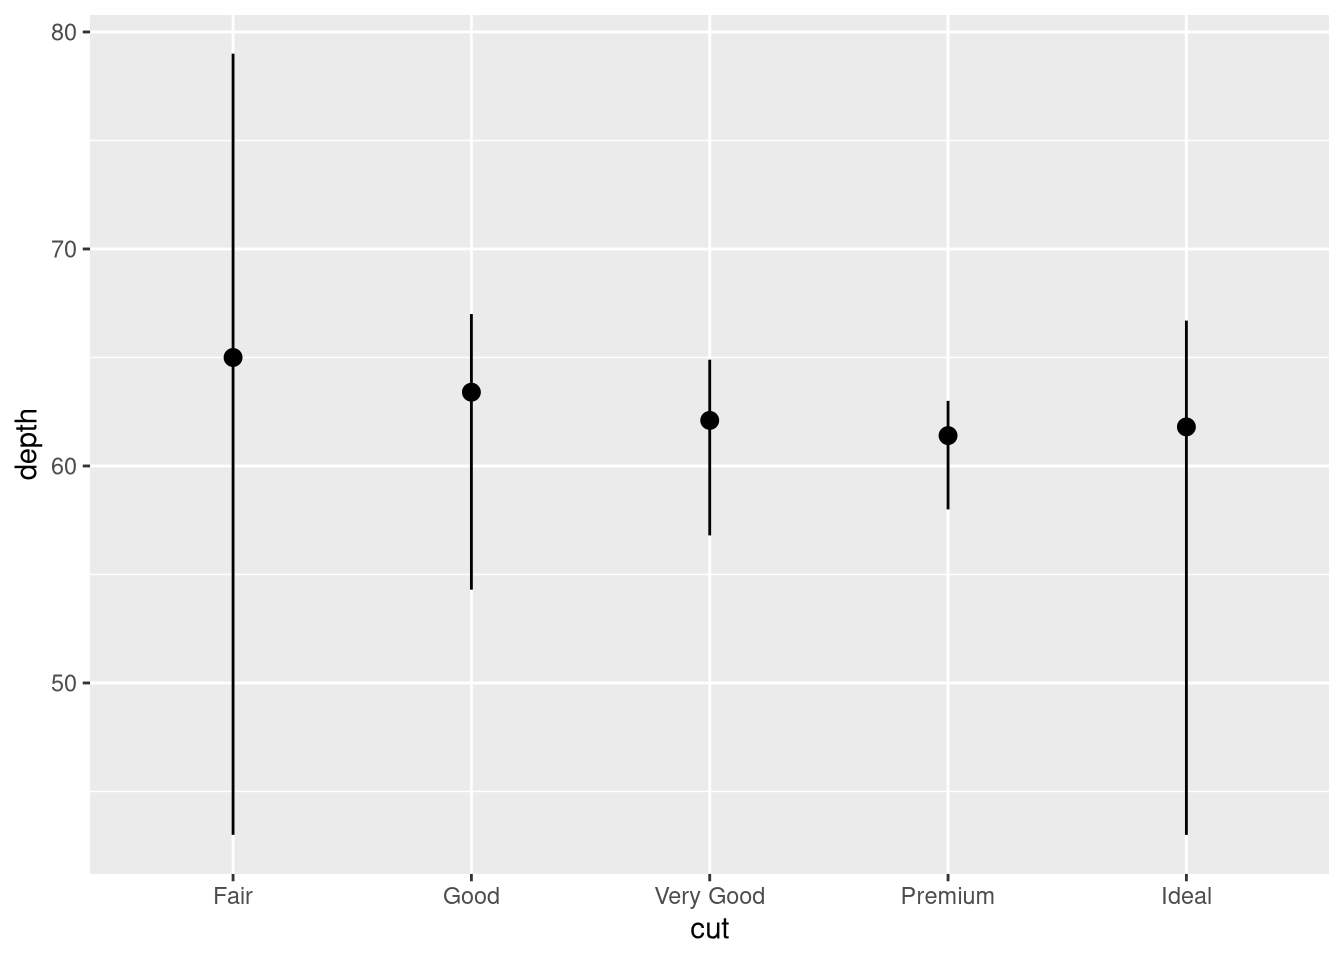
\includegraphics{CH09_files/figure-pdf/unnamed-chunk-28-1.pdf}

  }

  \end{figure}

  \begin{tcolorbox}[enhanced jigsaw, breakable, bottomtitle=1mm, left=2mm, colback=white, toprule=.15mm, leftrule=.75mm, colframe=quarto-callout-note-color-frame, colbacktitle=quarto-callout-note-color!10!white, title={Answer}, coltitle=black, toptitle=1mm, bottomrule=.15mm, opacitybacktitle=0.6, arc=.35mm, rightrule=.15mm, titlerule=0mm, opacityback=0]

  \emph{Your text answer here.}

\begin{Shaded}
\begin{Highlighting}[]
\NormalTok{diamonds }\SpecialCharTok{|\textgreater{}}
  \FunctionTok{group\_by}\NormalTok{(cut) }\SpecialCharTok{|\textgreater{}}
  \FunctionTok{summarize}\NormalTok{(}
    \AttributeTok{lower =} \FunctionTok{min}\NormalTok{(depth),}
    \AttributeTok{upper =} \FunctionTok{max}\NormalTok{(depth),}
    \AttributeTok{midpoint =} \FunctionTok{median}\NormalTok{(depth)}
\NormalTok{  ) }\SpecialCharTok{|\textgreater{}}
  \FunctionTok{ggplot}\NormalTok{(}\FunctionTok{aes}\NormalTok{(}\AttributeTok{x =}\NormalTok{ cut, }\AttributeTok{y =}\NormalTok{ midpoint)) }\SpecialCharTok{+}
  \FunctionTok{geom\_pointrange}\NormalTok{(}\FunctionTok{aes}\NormalTok{(}\AttributeTok{ymin =}\NormalTok{ lower, }\AttributeTok{ymax =}\NormalTok{ upper))}
\end{Highlighting}
\end{Shaded}

  \begin{figure}[H]

  {\centering 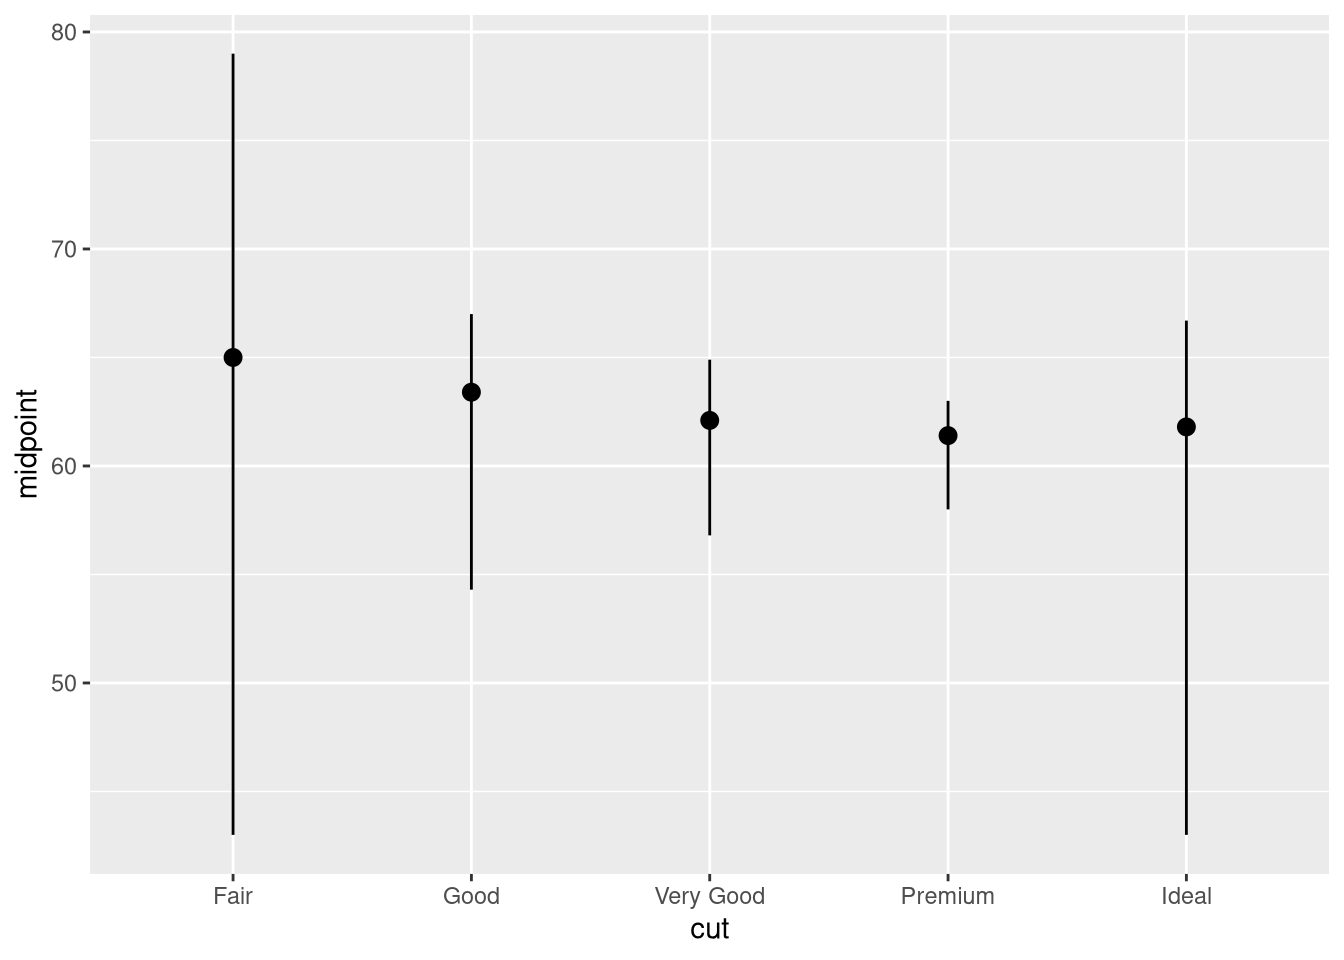
\includegraphics{CH09_files/figure-pdf/unnamed-chunk-29-1.pdf}

  }

  \end{figure}

  \end{tcolorbox}
\item
  What does \texttt{geom\_col()} do? How is it different from
  \texttt{geom\_bar()}?

  \begin{tcolorbox}[enhanced jigsaw, breakable, bottomtitle=1mm, left=2mm, colback=white, toprule=.15mm, leftrule=.75mm, colframe=quarto-callout-note-color-frame, colbacktitle=quarto-callout-note-color!10!white, title={Answer}, coltitle=black, toptitle=1mm, bottomrule=.15mm, opacitybacktitle=0.6, arc=.35mm, rightrule=.15mm, titlerule=0mm, opacityback=0]

  \emph{Your text answer here.}

  \end{tcolorbox}
\item
  Most geoms and stats come in pairs that are almost always used in
  concert. Make a list of all the pairs. What do they have in common?
  (Hint: Read through the documentation.)

  \begin{tcolorbox}[enhanced jigsaw, breakable, bottomtitle=1mm, left=2mm, colback=white, toprule=.15mm, leftrule=.75mm, colframe=quarto-callout-note-color-frame, colbacktitle=quarto-callout-note-color!10!white, title={Answer}, coltitle=black, toptitle=1mm, bottomrule=.15mm, opacitybacktitle=0.6, arc=.35mm, rightrule=.15mm, titlerule=0mm, opacityback=0]

  Geoms and stats that are almost always used in concert are listed
  below:

  \end{tcolorbox}

  \begin{longtable}[]{@{}ll@{}}
  \toprule\noalign{}
  \textbf{geom} & \textbf{stat} \\
  \midrule\noalign{}
  \endhead
  \bottomrule\noalign{}
  \endlastfoot
  \texttt{geom\_bar()} & \texttt{stat\_count()} \\
  \texttt{geom\_bin2d()} & \texttt{stat\_bin\_2d()} \\
  \texttt{geom\_boxplot()} & \texttt{stat\_boxplot()} \\
  \texttt{geom\_contour\_filled()} & \texttt{stat\_contour\_filled()} \\
  \texttt{geom\_contour()} & \texttt{stat\_contour()} \\
  \texttt{geom\_count()} & \texttt{stat\_sum()} \\
  \texttt{geom\_density\_2d()} & \texttt{stat\_density\_2d()} \\
  \texttt{geom\_density()} & \texttt{stat\_density()} \\
  \texttt{geom\_dotplot()} & \texttt{stat\_bindot()} \\
  \texttt{geom\_function()} & \texttt{stat\_function()} \\
  \texttt{geom\_sf()} & \texttt{stat\_sf()} \\
  \texttt{geom\_sf()} & \texttt{stat\_sf()} \\
  \texttt{geom\_smooth()} & \texttt{stat\_smooth()} \\
  \texttt{geom\_violin()} & \texttt{stat\_ydensity()} \\
  \texttt{geom\_hex()} & \texttt{stat\_bin\_hex()} \\
  \texttt{geom\_qq\_line()} & \texttt{stat\_qq\_line()} \\
  \texttt{geom\_qq()} & \texttt{stat\_qq()} \\
  \texttt{geom\_quantile()} & \texttt{stat\_quantile()} \\
  \end{longtable}
\item
  What variables does \texttt{stat\_smooth()} compute? What arguments
  control its behavior?

  \begin{tcolorbox}[enhanced jigsaw, breakable, bottomtitle=1mm, left=2mm, colback=white, toprule=.15mm, leftrule=.75mm, colframe=quarto-callout-note-color-frame, colbacktitle=quarto-callout-note-color!10!white, title={Answer}, coltitle=black, toptitle=1mm, bottomrule=.15mm, opacitybacktitle=0.6, arc=.35mm, rightrule=.15mm, titlerule=0mm, opacityback=0]

  \texttt{stat\_smooth()} computes the following variables:

  \begin{itemize}
  \tightlist
  \item
    \texttt{y} or \texttt{x}: Predicted value
  \item
    \texttt{ymin} or \texttt{xmin}: Lower pointwise confidence interval
    around the mean
  \item
    \texttt{ymax} or \texttt{xmax}: Upper pointwise confidence interval
    around the mean
  \item
    \texttt{se}: Standard error
  \end{itemize}

  \end{tcolorbox}
\item
  In our proportion bar chart, we needed to set \texttt{group\ =\ 1}.
  Why? In other words, what is the problem with these two graphs?

\begin{Shaded}
\begin{Highlighting}[]
\FunctionTok{ggplot}\NormalTok{(diamonds, }\FunctionTok{aes}\NormalTok{(}\AttributeTok{x =}\NormalTok{ cut, }\AttributeTok{y =} \FunctionTok{after\_stat}\NormalTok{(prop))) }\SpecialCharTok{+} 
  \FunctionTok{geom\_bar}\NormalTok{()}
\end{Highlighting}
\end{Shaded}

\begin{Shaded}
\begin{Highlighting}[]
\FunctionTok{ggplot}\NormalTok{(diamonds, }\FunctionTok{aes}\NormalTok{(}\AttributeTok{x =}\NormalTok{ cut, }\AttributeTok{fill =}\NormalTok{ color, }\AttributeTok{y =} \FunctionTok{after\_stat}\NormalTok{(prop))) }\SpecialCharTok{+} 
  \FunctionTok{geom\_bar}\NormalTok{()}
\end{Highlighting}
\end{Shaded}

  \begin{tcolorbox}[enhanced jigsaw, breakable, bottomtitle=1mm, left=2mm, colback=white, toprule=.15mm, leftrule=.75mm, colframe=quarto-callout-note-color-frame, colbacktitle=quarto-callout-note-color!10!white, title={Answer}, coltitle=black, toptitle=1mm, bottomrule=.15mm, opacitybacktitle=0.6, arc=.35mm, rightrule=.15mm, titlerule=0mm, opacityback=0]

  \emph{Your text answer here.}

  \end{tcolorbox}

\begin{Shaded}
\begin{Highlighting}[]
\CommentTok{\# one variable}
\FunctionTok{ggplot}\NormalTok{(diamonds, }\FunctionTok{aes}\NormalTok{(}\AttributeTok{x =}\NormalTok{ cut, }
                     \AttributeTok{y =} \FunctionTok{after\_stat}\NormalTok{(prop))) }\SpecialCharTok{+} 
  \FunctionTok{geom\_bar}\NormalTok{()}
\FunctionTok{ggplot}\NormalTok{(diamonds, }\FunctionTok{aes}\NormalTok{(}\AttributeTok{x =}\NormalTok{ cut, }
                     \AttributeTok{y =} \FunctionTok{after\_stat}\NormalTok{(prop), }
                     \AttributeTok{group =} \DecValTok{1}\NormalTok{)) }\SpecialCharTok{+} 
  \FunctionTok{geom\_bar}\NormalTok{()}
\CommentTok{\# two variables}
\FunctionTok{ggplot}\NormalTok{(diamonds, }\FunctionTok{aes}\NormalTok{(}\AttributeTok{x =}\NormalTok{ cut, }
                     \AttributeTok{fill =}\NormalTok{ color, }
                     \AttributeTok{y =} \FunctionTok{after\_stat}\NormalTok{(prop))) }\SpecialCharTok{+} 
  \FunctionTok{geom\_bar}\NormalTok{()}
\FunctionTok{ggplot}\NormalTok{(diamonds, }\FunctionTok{aes}\NormalTok{(}\AttributeTok{x =}\NormalTok{ cut, }
                     \AttributeTok{fill =}\NormalTok{ color, }
                     \AttributeTok{y =} \FunctionTok{after\_stat}\NormalTok{(prop), }
                     \AttributeTok{group =}\NormalTok{ color)) }\SpecialCharTok{+} 
  \FunctionTok{geom\_bar}\NormalTok{()}
\end{Highlighting}
\end{Shaded}

  \begin{figure}

  \begin{minipage}[t]{0.50\linewidth}

  {\centering 

  \raisebox{-\height}{

  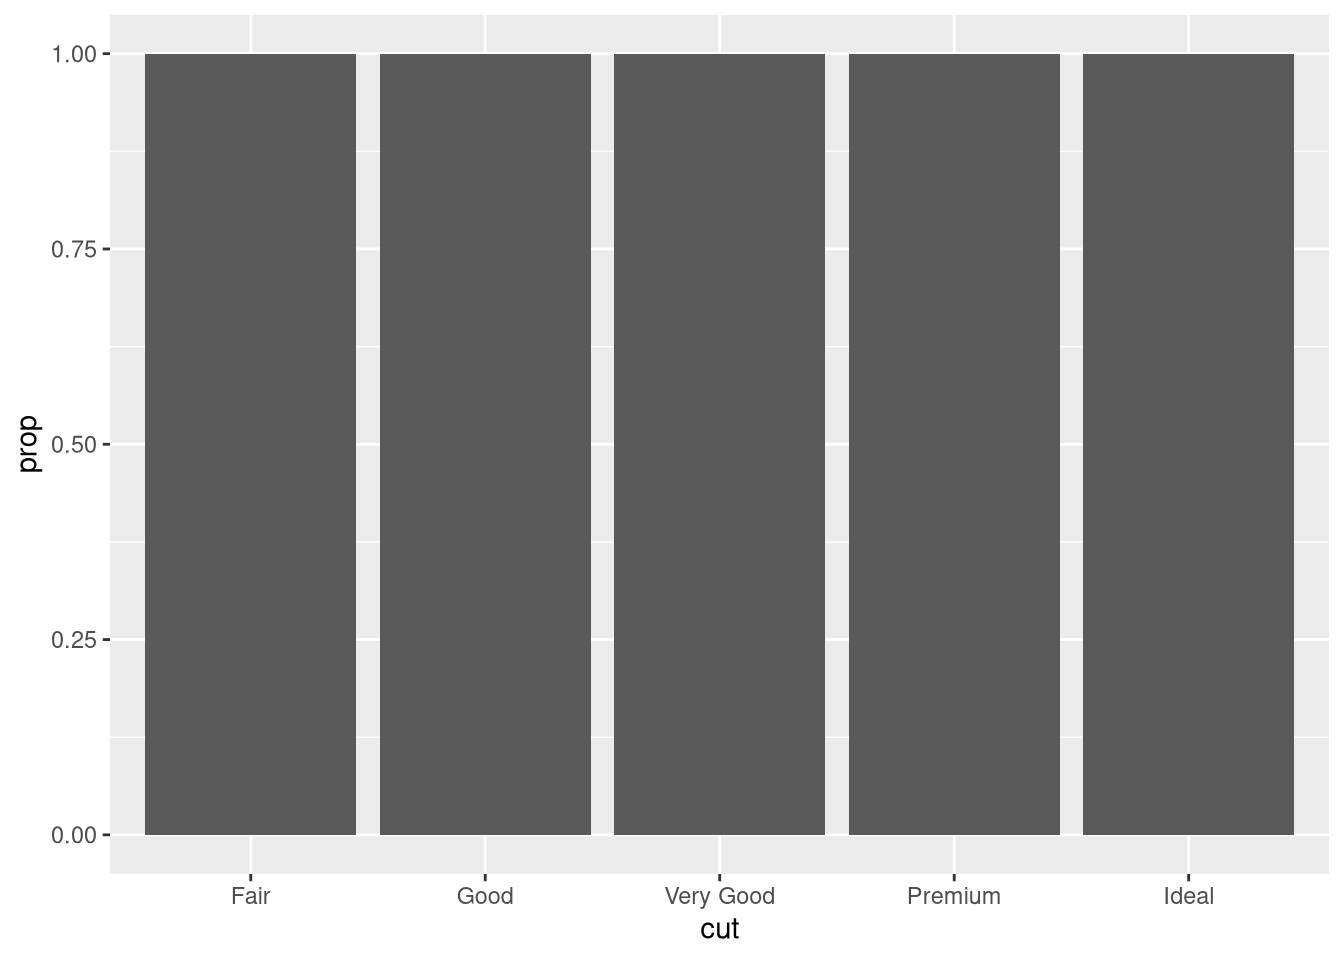
\includegraphics{CH09_files/figure-pdf/unnamed-chunk-31-1.pdf}

  }

  }

  \end{minipage}%
  %
  \begin{minipage}[t]{0.50\linewidth}

  {\centering 

  \raisebox{-\height}{

  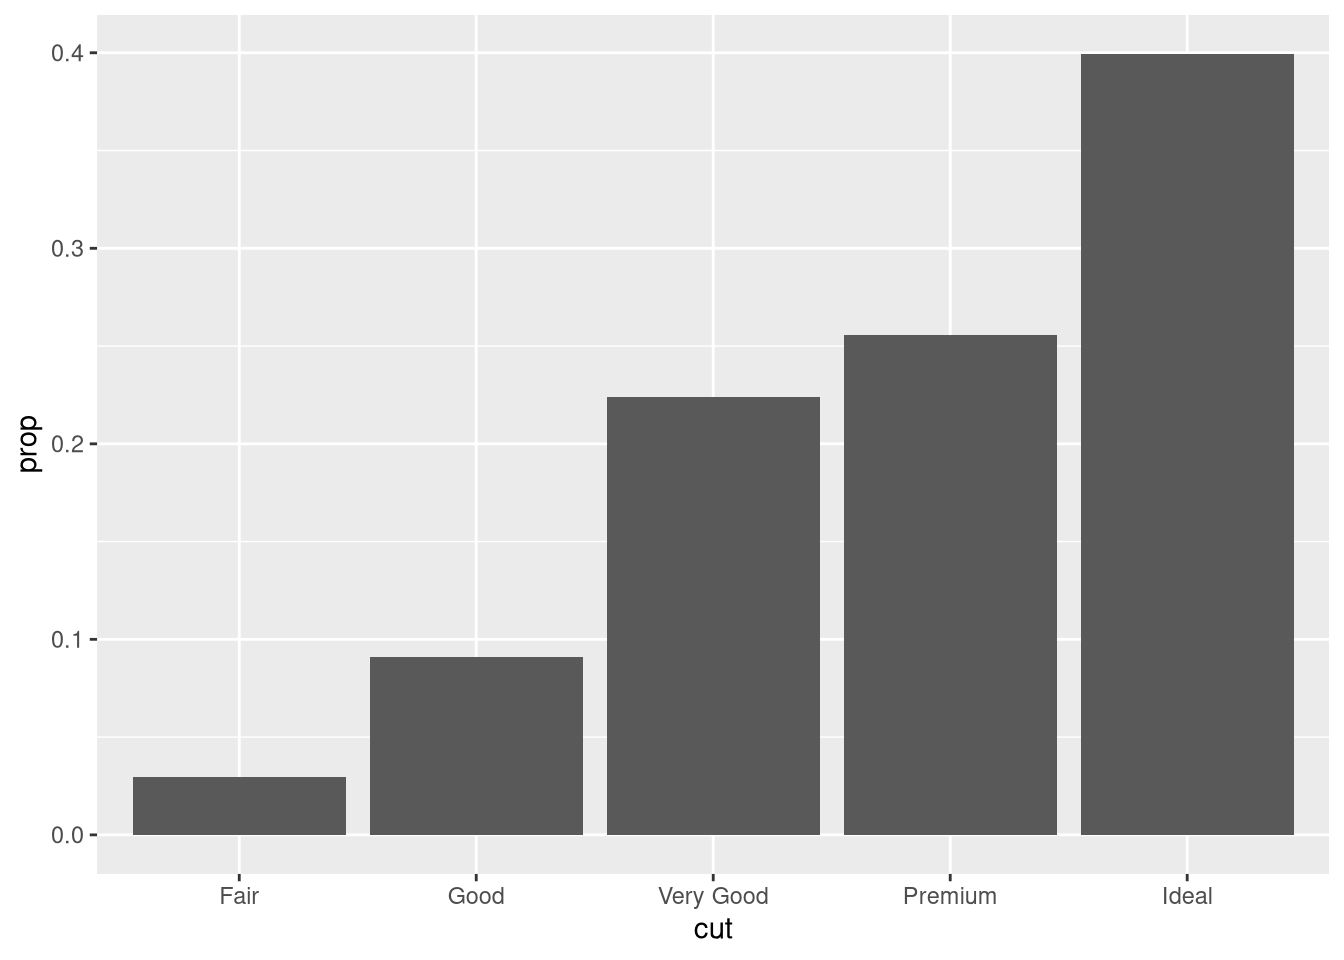
\includegraphics{CH09_files/figure-pdf/unnamed-chunk-31-2.pdf}

  }

  }

  \end{minipage}%
  \newline
  \begin{minipage}[t]{0.50\linewidth}

  {\centering 

  \raisebox{-\height}{

  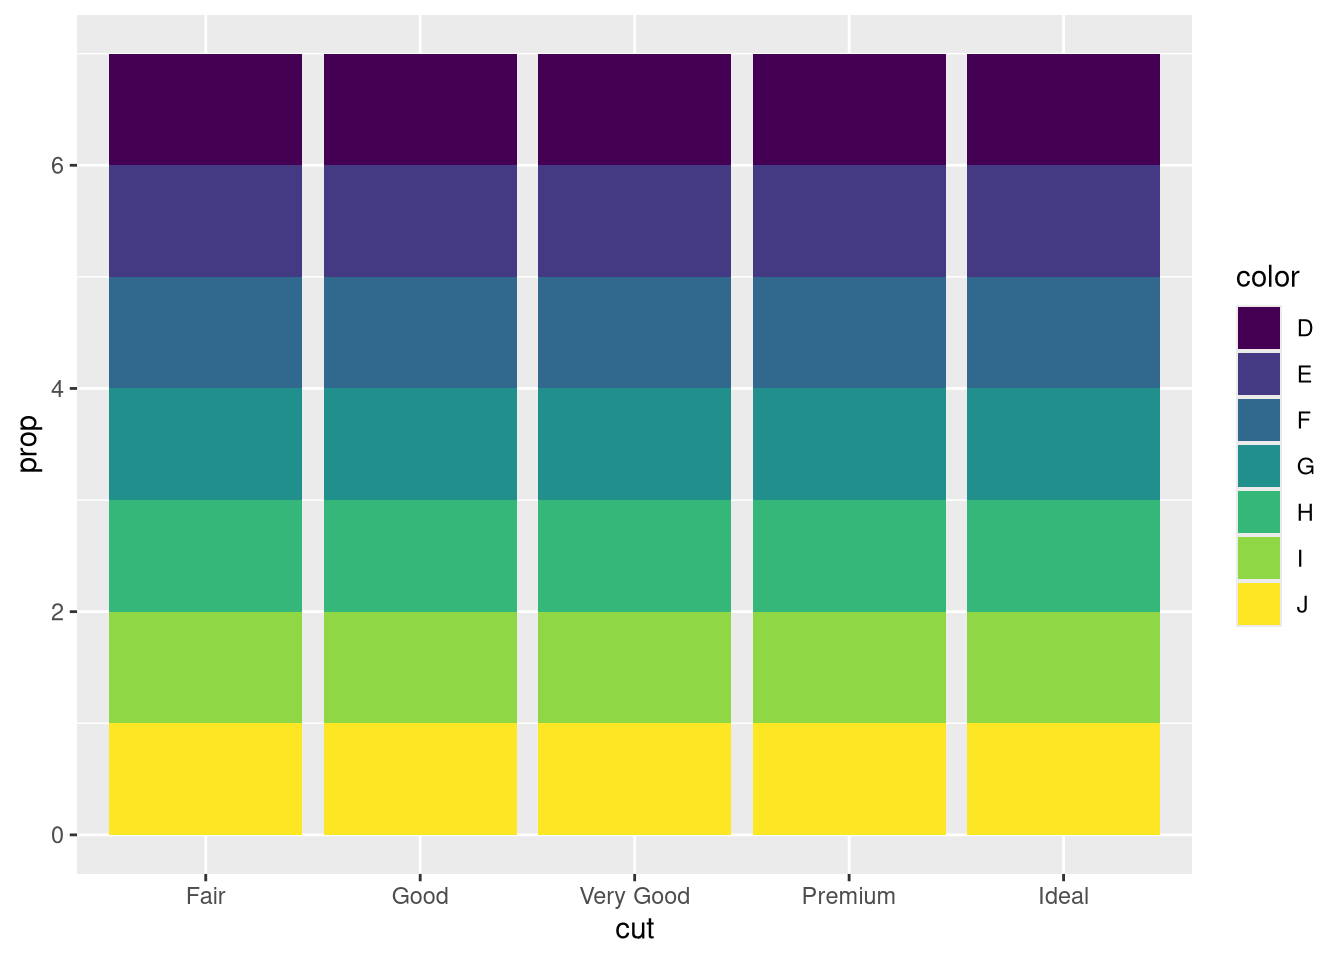
\includegraphics{CH09_files/figure-pdf/unnamed-chunk-31-3.pdf}

  }

  }

  \end{minipage}%
  %
  \begin{minipage}[t]{0.50\linewidth}

  {\centering 

  \raisebox{-\height}{

  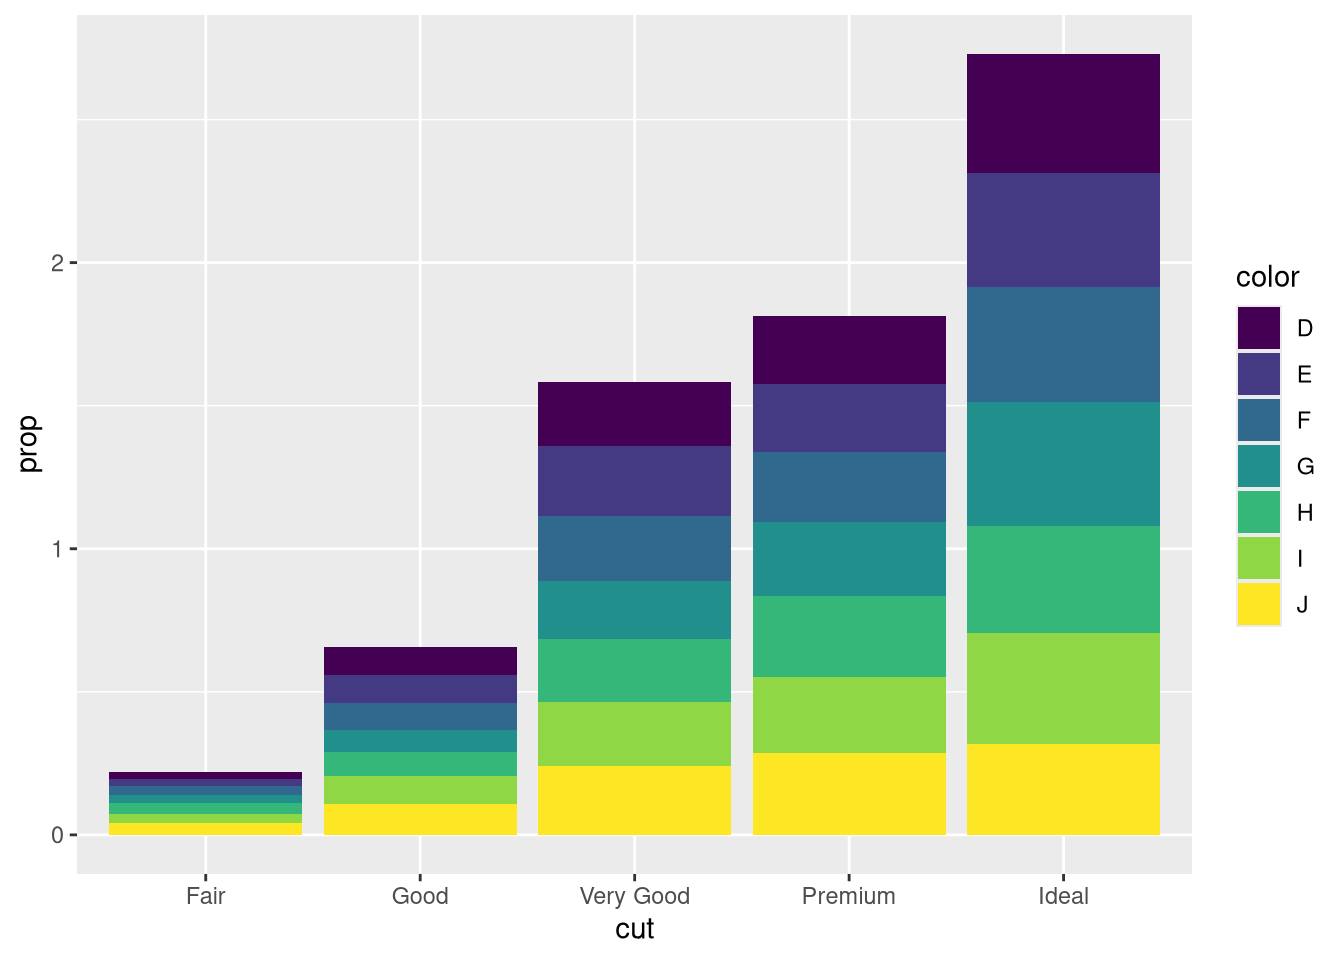
\includegraphics{CH09_files/figure-pdf/unnamed-chunk-31-4.pdf}

  }

  }

  \end{minipage}%

  \end{figure}
\item
  What is the problem with the following plot? How could you improve it?

\begin{Shaded}
\begin{Highlighting}[]
\FunctionTok{ggplot}\NormalTok{(mpg, }\FunctionTok{aes}\NormalTok{(}\AttributeTok{x =}\NormalTok{ cty, }\AttributeTok{y =}\NormalTok{ hwy)) }\SpecialCharTok{+} 
  \FunctionTok{geom\_point}\NormalTok{()}
\end{Highlighting}
\end{Shaded}

  \begin{tcolorbox}[enhanced jigsaw, breakable, bottomtitle=1mm, left=2mm, colback=white, toprule=.15mm, leftrule=.75mm, colframe=quarto-callout-note-color-frame, colbacktitle=quarto-callout-note-color!10!white, title={Answer}, coltitle=black, toptitle=1mm, bottomrule=.15mm, opacitybacktitle=0.6, arc=.35mm, rightrule=.15mm, titlerule=0mm, opacityback=0]

  \emph{Your text answer here.}

  \end{tcolorbox}

\begin{Shaded}
\begin{Highlighting}[]
\FunctionTok{ggplot}\NormalTok{(mpg, }\FunctionTok{aes}\NormalTok{(}\AttributeTok{x =}\NormalTok{ cty, }\AttributeTok{y =}\NormalTok{ hwy)) }\SpecialCharTok{+} 
  \FunctionTok{geom\_point}\NormalTok{()}
\FunctionTok{ggplot}\NormalTok{(mpg, }\FunctionTok{aes}\NormalTok{(}\AttributeTok{x =}\NormalTok{ cty, }\AttributeTok{y =}\NormalTok{ hwy)) }\SpecialCharTok{+} 
  \FunctionTok{geom\_jitter}\NormalTok{()}
\end{Highlighting}
\end{Shaded}

  \begin{figure}

  \begin{minipage}[t]{0.50\linewidth}

  {\centering 

  \raisebox{-\height}{

  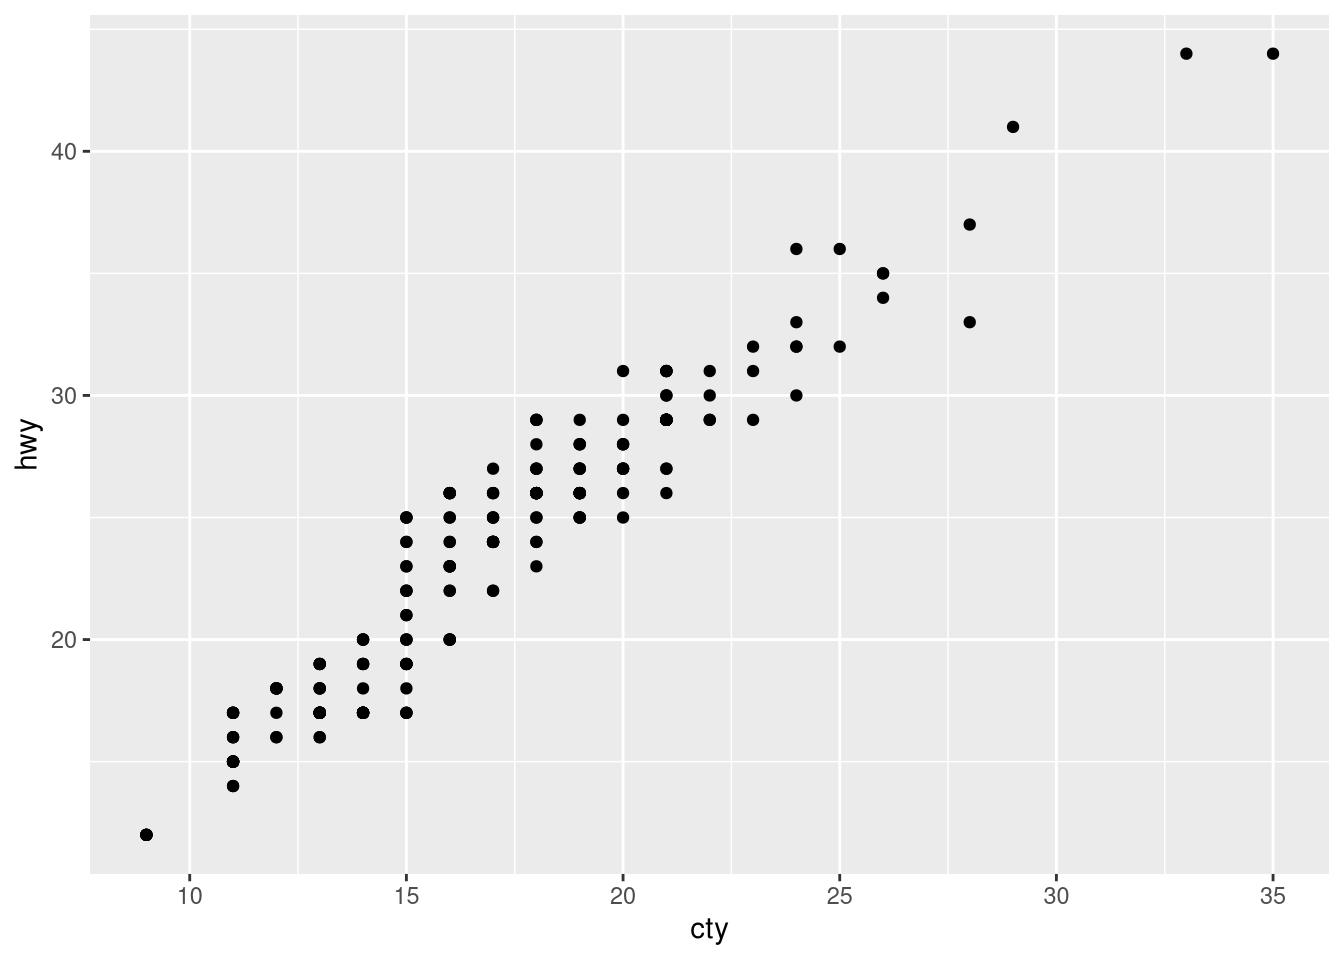
\includegraphics{CH09_files/figure-pdf/unnamed-chunk-33-1.pdf}

  }

  }

  \end{minipage}%
  %
  \begin{minipage}[t]{0.50\linewidth}

  {\centering 

  \raisebox{-\height}{

  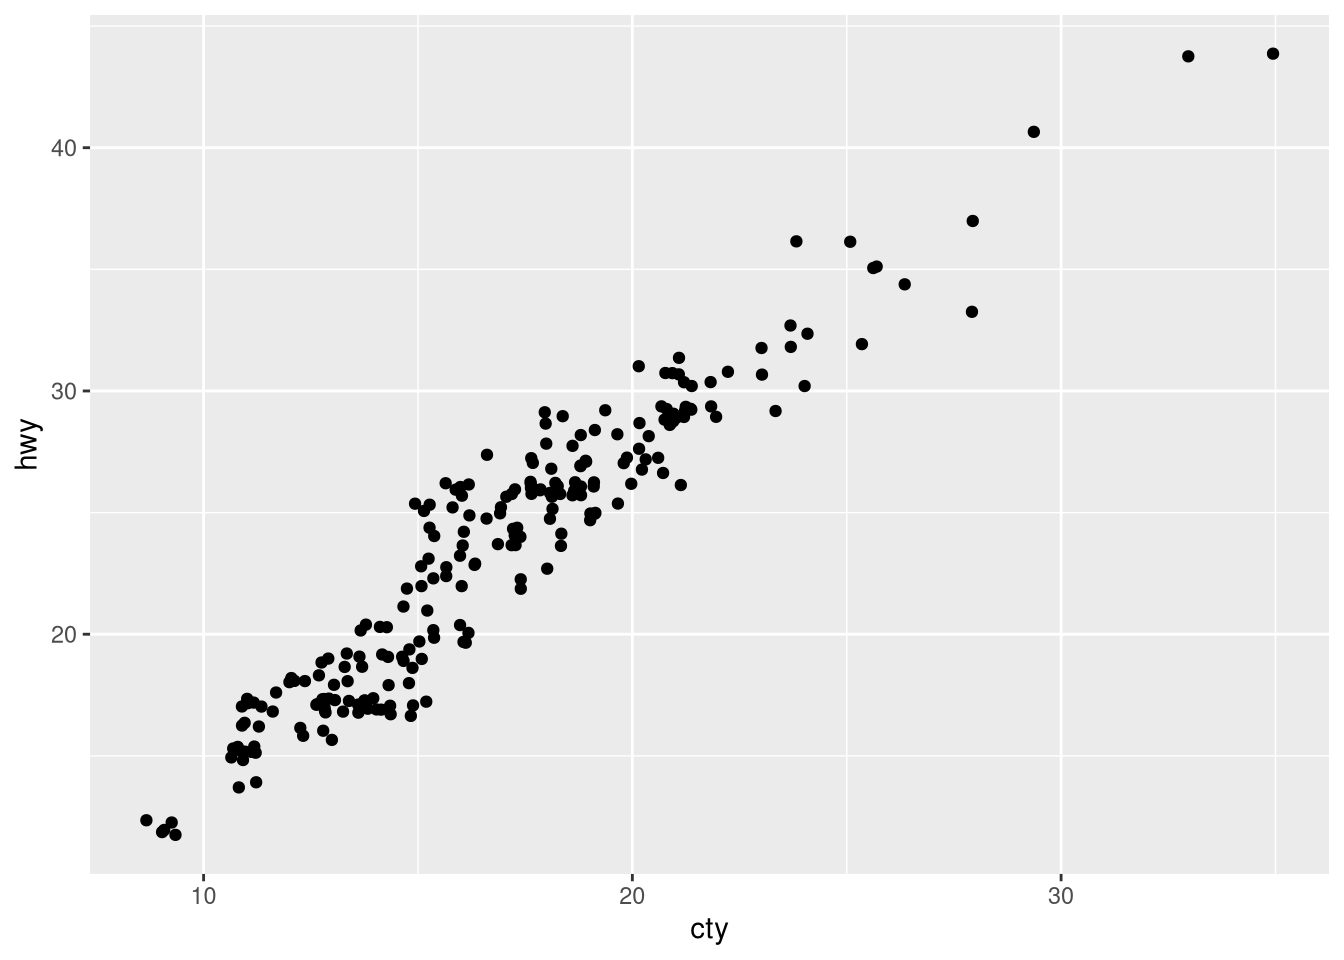
\includegraphics{CH09_files/figure-pdf/unnamed-chunk-33-2.pdf}

  }

  }

  \end{minipage}%

  \end{figure}
\item
  What, if anything, is the difference between the two plots? Why?

\begin{Shaded}
\begin{Highlighting}[]
\FunctionTok{ggplot}\NormalTok{(mpg, }\FunctionTok{aes}\NormalTok{(}\AttributeTok{x =}\NormalTok{ displ, }\AttributeTok{y =}\NormalTok{ hwy)) }\SpecialCharTok{+}
  \FunctionTok{geom\_point}\NormalTok{()}
\end{Highlighting}
\end{Shaded}

\begin{Shaded}
\begin{Highlighting}[]
\FunctionTok{ggplot}\NormalTok{(mpg, }\FunctionTok{aes}\NormalTok{(}\AttributeTok{x =}\NormalTok{ displ, }\AttributeTok{y =}\NormalTok{ hwy)) }\SpecialCharTok{+}
  \FunctionTok{geom\_point}\NormalTok{(}\AttributeTok{position =} \StringTok{"identity"}\NormalTok{)}
\end{Highlighting}
\end{Shaded}

  \begin{tcolorbox}[enhanced jigsaw, breakable, bottomtitle=1mm, left=2mm, colback=white, toprule=.15mm, leftrule=.75mm, colframe=quarto-callout-note-color-frame, colbacktitle=quarto-callout-note-color!10!white, title={Answer}, coltitle=black, toptitle=1mm, bottomrule=.15mm, opacitybacktitle=0.6, arc=.35mm, rightrule=.15mm, titlerule=0mm, opacityback=0]

  \emph{Your text answer here.}

  \end{tcolorbox}

\begin{Shaded}
\begin{Highlighting}[]
\CommentTok{\# Your R code here}
\end{Highlighting}
\end{Shaded}

  \begin{figure}

  \end{figure}
\item
  What parameters to \texttt{geom\_jitter()} control the amount of
  jittering?

  \begin{tcolorbox}[enhanced jigsaw, breakable, bottomtitle=1mm, left=2mm, colback=white, toprule=.15mm, leftrule=.75mm, colframe=quarto-callout-note-color-frame, colbacktitle=quarto-callout-note-color!10!white, title={Answer}, coltitle=black, toptitle=1mm, bottomrule=.15mm, opacitybacktitle=0.6, arc=.35mm, rightrule=.15mm, titlerule=0mm, opacityback=0]

  \emph{Your text answer here.}

  \end{tcolorbox}

\begin{Shaded}
\begin{Highlighting}[]
\FunctionTok{set.seed}\NormalTok{(}\DecValTok{321}\NormalTok{)}
\FunctionTok{ggplot}\NormalTok{(mpg, }\FunctionTok{aes}\NormalTok{(}\AttributeTok{x =}\NormalTok{ displ, }\AttributeTok{y =}\NormalTok{ hwy)) }\SpecialCharTok{+}
  \FunctionTok{geom\_point}\NormalTok{(}\AttributeTok{color =} \StringTok{"gray"}\NormalTok{) }\SpecialCharTok{+}
  \FunctionTok{geom\_jitter}\NormalTok{(}\AttributeTok{height =} \DecValTok{1}\NormalTok{, }\AttributeTok{width =} \DecValTok{1}\NormalTok{)}
\FunctionTok{ggplot}\NormalTok{(mpg, }\FunctionTok{aes}\NormalTok{(}\AttributeTok{x =}\NormalTok{ displ, }\AttributeTok{y =}\NormalTok{ hwy)) }\SpecialCharTok{+}
  \FunctionTok{geom\_point}\NormalTok{(}\AttributeTok{color =} \StringTok{"gray"}\NormalTok{) }\SpecialCharTok{+}
  \FunctionTok{geom\_jitter}\NormalTok{(}\AttributeTok{height =} \DecValTok{1}\NormalTok{, }\AttributeTok{width =} \DecValTok{5}\NormalTok{)}
\FunctionTok{ggplot}\NormalTok{(mpg, }\FunctionTok{aes}\NormalTok{(}\AttributeTok{x =}\NormalTok{ displ, }\AttributeTok{y =}\NormalTok{ hwy)) }\SpecialCharTok{+}
  \FunctionTok{geom\_point}\NormalTok{(}\AttributeTok{color =} \StringTok{"gray"}\NormalTok{) }\SpecialCharTok{+}
  \FunctionTok{geom\_jitter}\NormalTok{(}\AttributeTok{height =} \DecValTok{5}\NormalTok{, }\AttributeTok{width =} \DecValTok{1}\NormalTok{)}
\end{Highlighting}
\end{Shaded}

  \begin{figure}

  \begin{minipage}[t]{0.33\linewidth}

  {\centering 

  \raisebox{-\height}{

  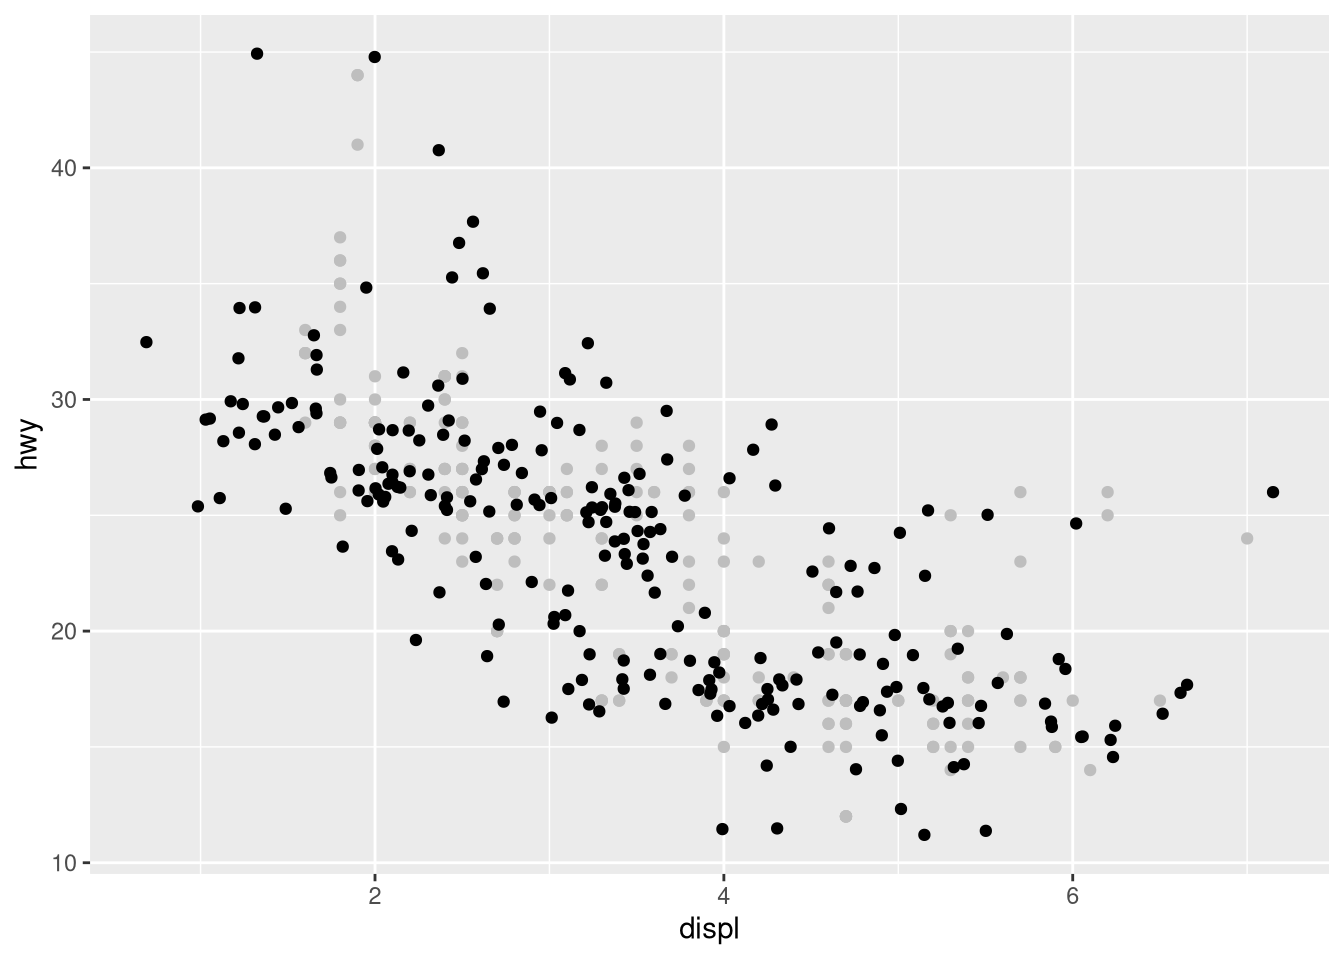
\includegraphics{CH09_files/figure-pdf/unnamed-chunk-36-1.pdf}

  }

  }

  \end{minipage}%
  %
  \begin{minipage}[t]{0.33\linewidth}

  {\centering 

  \raisebox{-\height}{

  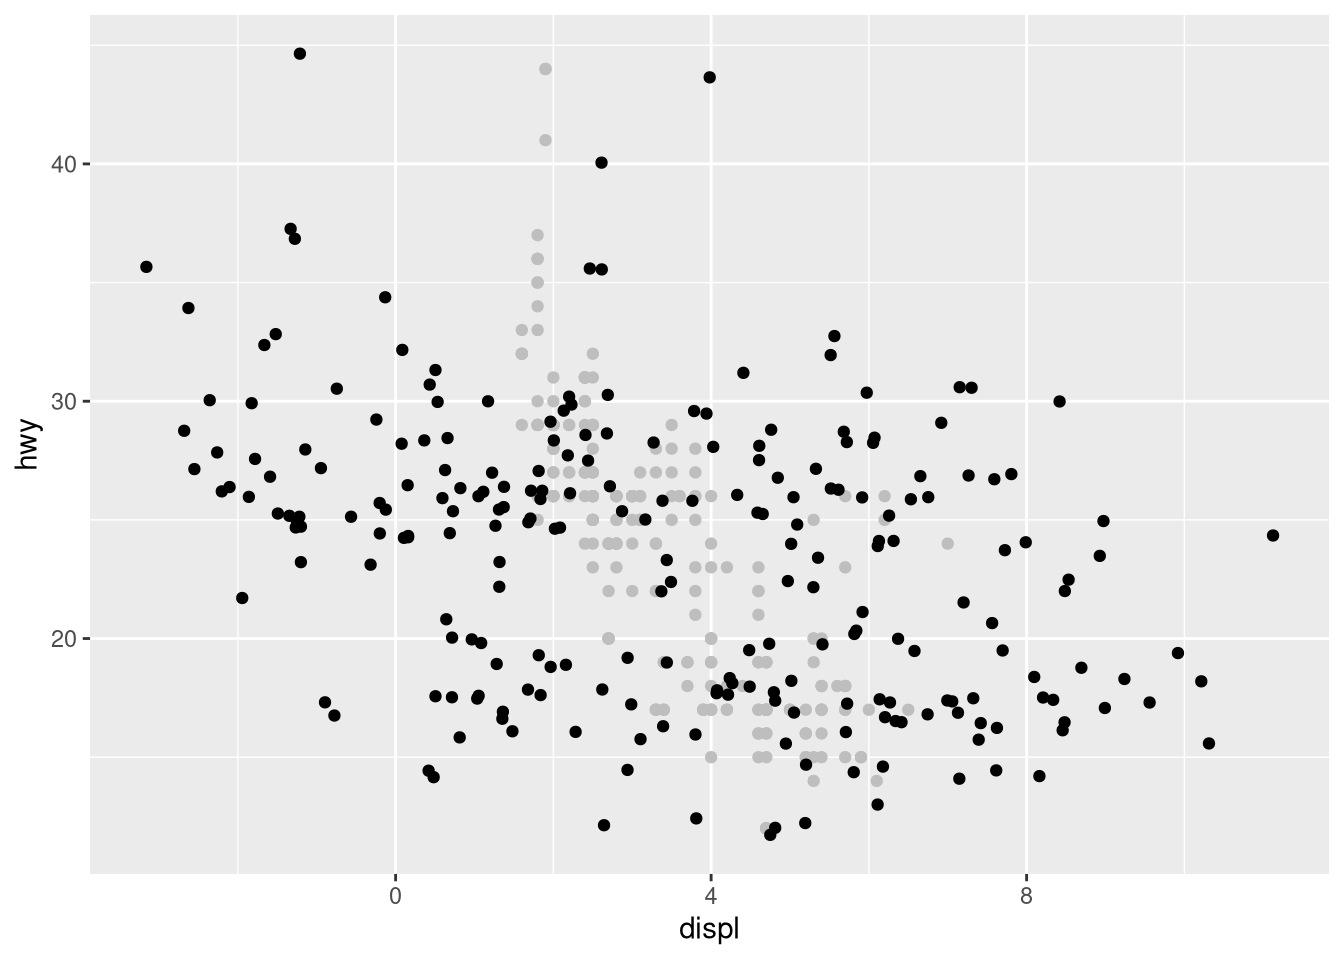
\includegraphics{CH09_files/figure-pdf/unnamed-chunk-36-2.pdf}

  }

  }

  \end{minipage}%
  %
  \begin{minipage}[t]{0.33\linewidth}

  {\centering 

  \raisebox{-\height}{

  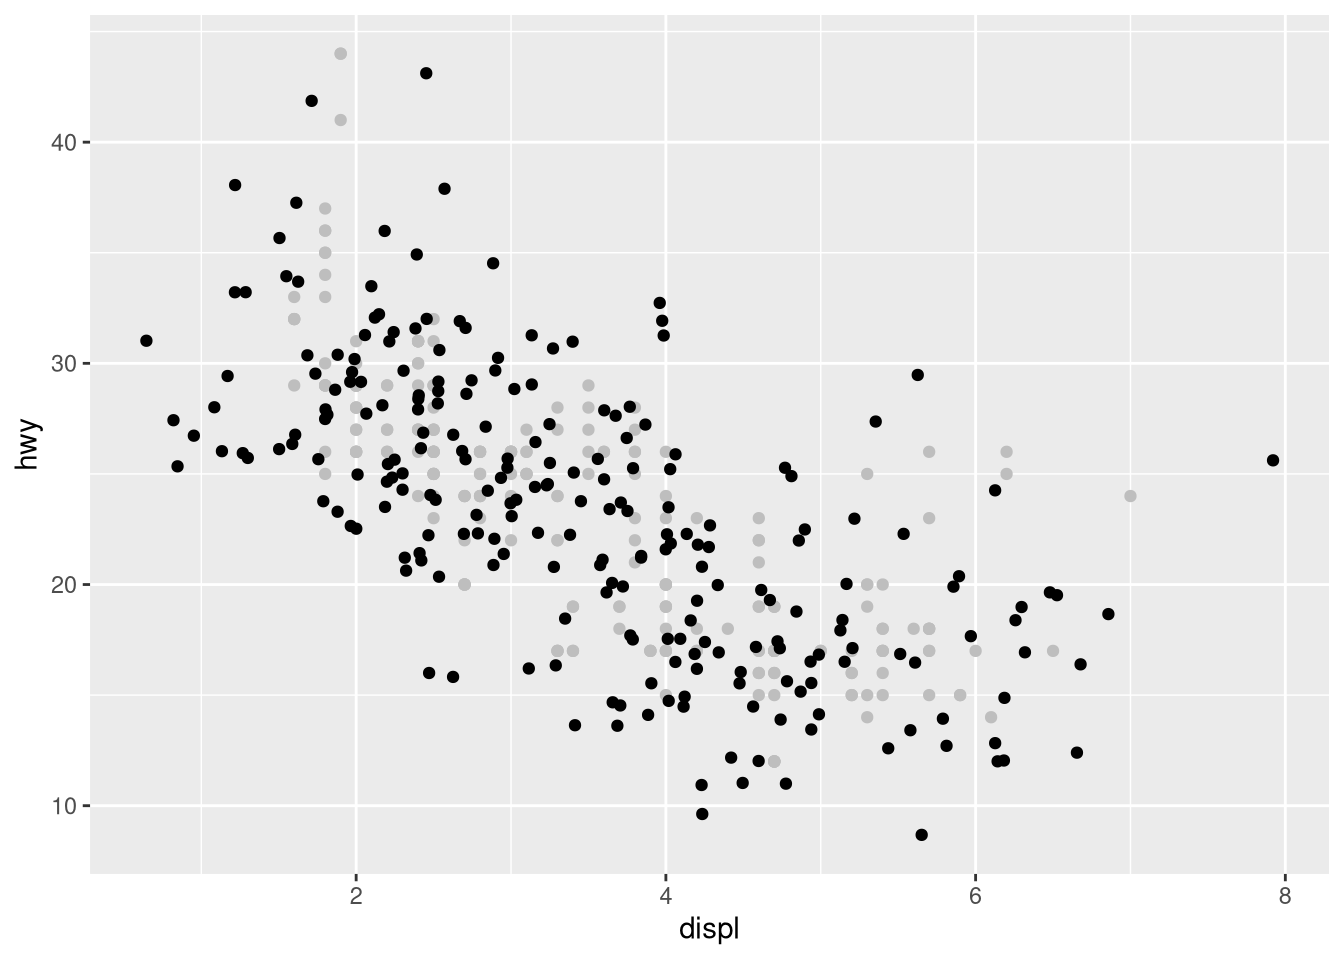
\includegraphics{CH09_files/figure-pdf/unnamed-chunk-36-3.pdf}

  }

  }

  \end{minipage}%

  \end{figure}
\item
  Compare and contrast \texttt{geom\_jitter()} with
  \texttt{geom\_count()}.

  \begin{tcolorbox}[enhanced jigsaw, breakable, bottomtitle=1mm, left=2mm, colback=white, toprule=.15mm, leftrule=.75mm, colframe=quarto-callout-note-color-frame, colbacktitle=quarto-callout-note-color!10!white, title={Answer}, coltitle=black, toptitle=1mm, bottomrule=.15mm, opacitybacktitle=0.6, arc=.35mm, rightrule=.15mm, titlerule=0mm, opacityback=0]

  \emph{Your text answer here.}

  \end{tcolorbox}

\begin{Shaded}
\begin{Highlighting}[]
\FunctionTok{ggplot}\NormalTok{(mpg, }\FunctionTok{aes}\NormalTok{(}\AttributeTok{x =}\NormalTok{ displ, }\AttributeTok{y =}\NormalTok{ hwy)) }\SpecialCharTok{+}
  \FunctionTok{geom\_jitter}\NormalTok{()}
\FunctionTok{ggplot}\NormalTok{(mpg, }\FunctionTok{aes}\NormalTok{(}\AttributeTok{x =}\NormalTok{ displ, }\AttributeTok{y =}\NormalTok{ hwy)) }\SpecialCharTok{+}
  \FunctionTok{geom\_count}\NormalTok{()}
\end{Highlighting}
\end{Shaded}

  \begin{figure}

  \begin{minipage}[t]{0.50\linewidth}

  {\centering 

  \raisebox{-\height}{

  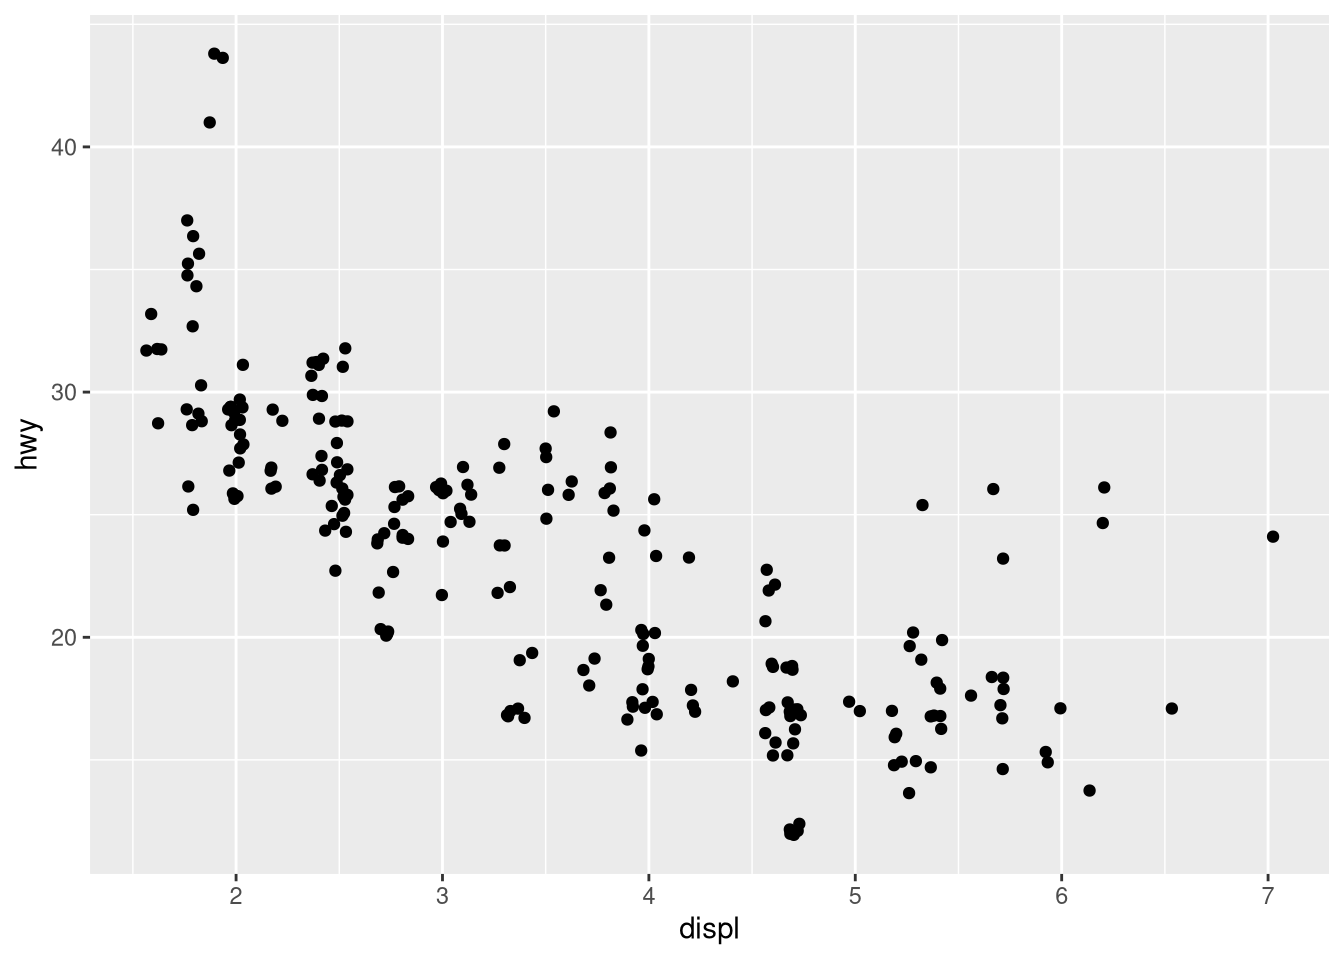
\includegraphics{CH09_files/figure-pdf/unnamed-chunk-37-1.pdf}

  }

  }

  \end{minipage}%
  %
  \begin{minipage}[t]{0.50\linewidth}

  {\centering 

  \raisebox{-\height}{

  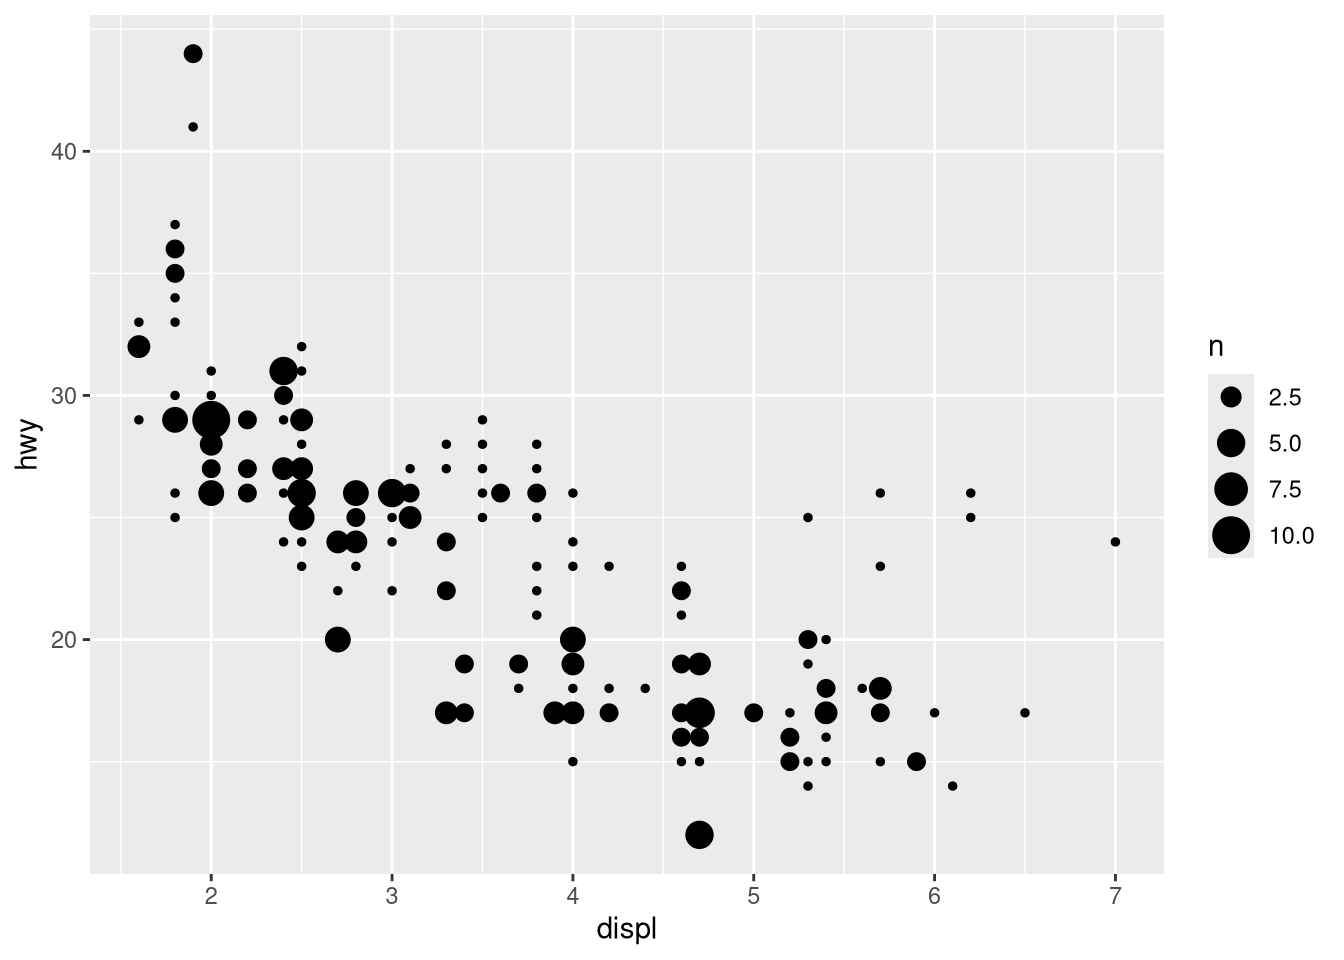
\includegraphics{CH09_files/figure-pdf/unnamed-chunk-37-2.pdf}

  }

  }

  \end{minipage}%

  \end{figure}
\item
  What's the default position adjustment for \texttt{geom\_boxplot()}?
  Create a visualization of the \texttt{mpg} dataset that demonstrates
  it.

  \begin{tcolorbox}[enhanced jigsaw, breakable, bottomtitle=1mm, left=2mm, colback=white, toprule=.15mm, leftrule=.75mm, colframe=quarto-callout-note-color-frame, colbacktitle=quarto-callout-note-color!10!white, title={Answer}, coltitle=black, toptitle=1mm, bottomrule=.15mm, opacitybacktitle=0.6, arc=.35mm, rightrule=.15mm, titlerule=0mm, opacityback=0]

  \emph{Your text answer here.}

  \end{tcolorbox}

\begin{Shaded}
\begin{Highlighting}[]
\FunctionTok{ggplot}\NormalTok{(mpg, }\FunctionTok{aes}\NormalTok{(}\AttributeTok{x =}\NormalTok{ drv, }\AttributeTok{y =}\NormalTok{ displ)) }\SpecialCharTok{+}
  \FunctionTok{geom\_boxplot}\NormalTok{()}
\FunctionTok{ggplot}\NormalTok{(mpg, }\FunctionTok{aes}\NormalTok{(}\AttributeTok{x =}\NormalTok{ drv, }\AttributeTok{y =}\NormalTok{ displ)) }\SpecialCharTok{+}
  \FunctionTok{geom\_boxplot}\NormalTok{(}\AttributeTok{position =} \StringTok{"dodge2"}\NormalTok{)}
\end{Highlighting}
\end{Shaded}

  \begin{figure}

  \begin{minipage}[t]{0.50\linewidth}

  {\centering 

  \raisebox{-\height}{

  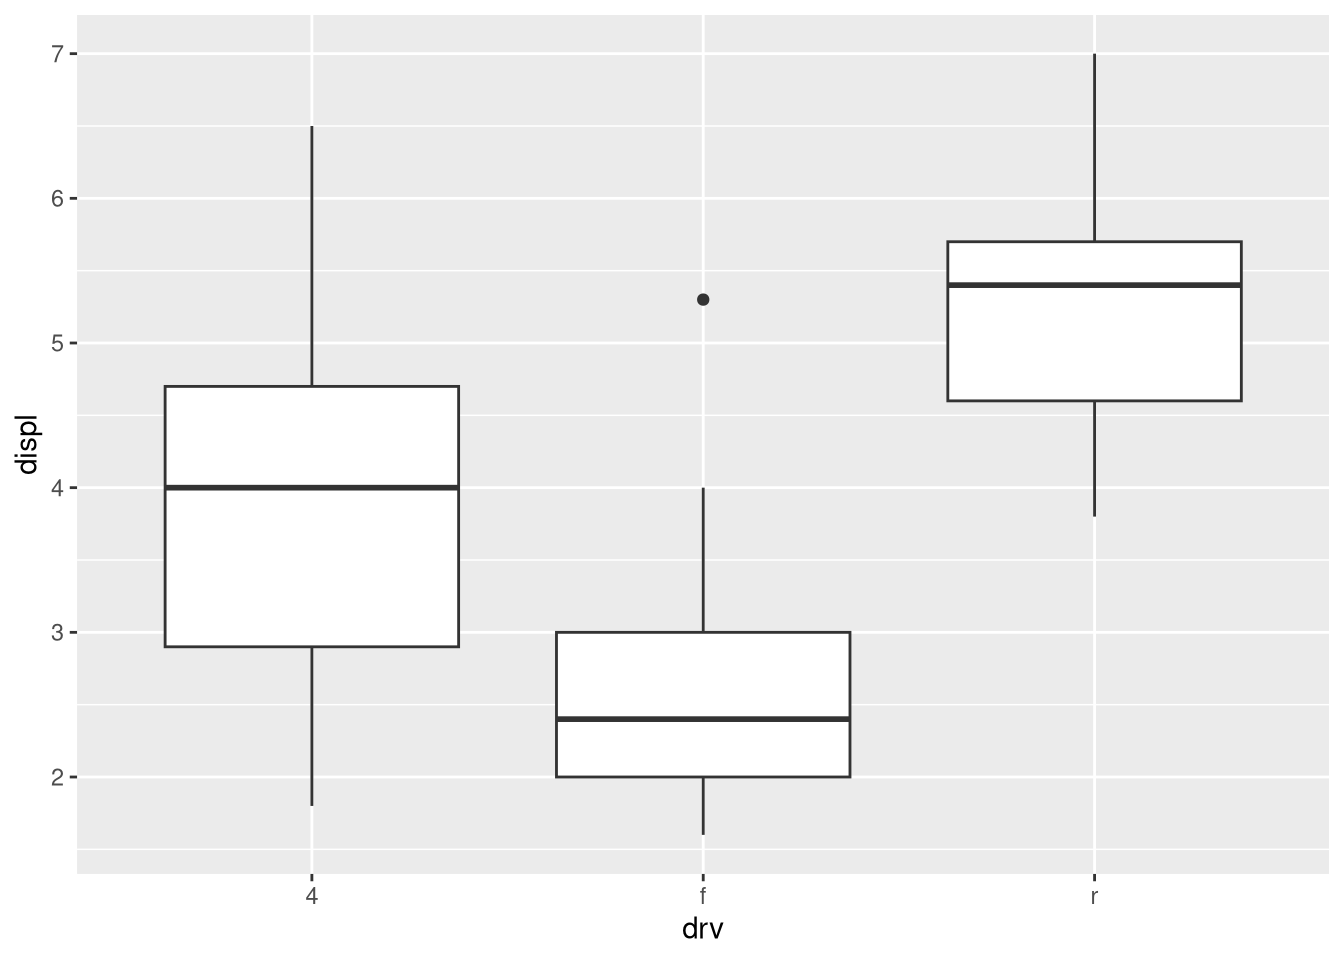
\includegraphics{CH09_files/figure-pdf/unnamed-chunk-38-1.pdf}

  }

  }

  \end{minipage}%
  %
  \begin{minipage}[t]{0.50\linewidth}

  {\centering 

  \raisebox{-\height}{

  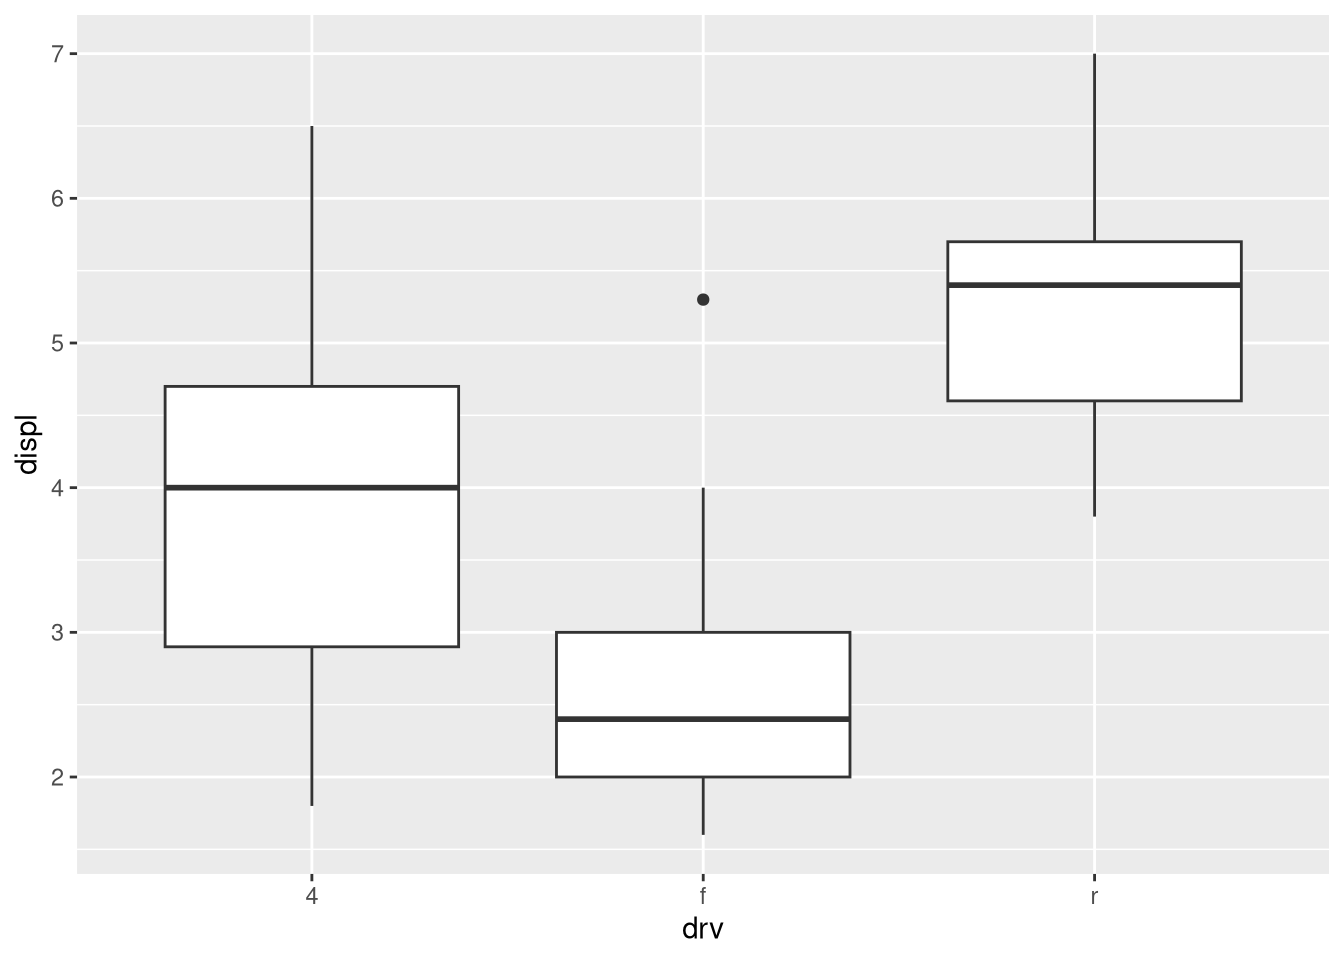
\includegraphics{CH09_files/figure-pdf/unnamed-chunk-38-2.pdf}

  }

  }

  \end{minipage}%

  \end{figure}
\item
  Turn a stacked bar chart into a pie chart using
  \texttt{coord\_polar()}.

  \begin{tcolorbox}[enhanced jigsaw, breakable, bottomtitle=1mm, left=2mm, colback=white, toprule=.15mm, leftrule=.75mm, colframe=quarto-callout-note-color-frame, colbacktitle=quarto-callout-note-color!10!white, title={Answer}, coltitle=black, toptitle=1mm, bottomrule=.15mm, opacitybacktitle=0.6, arc=.35mm, rightrule=.15mm, titlerule=0mm, opacityback=0]

  \emph{Your text answer here.}

  \end{tcolorbox}

\begin{Shaded}
\begin{Highlighting}[]
\CommentTok{\# Your R code here  }
\end{Highlighting}
\end{Shaded}

  \begin{figure}

  \end{figure}
\item
  What's the difference between \texttt{coord\_quickmap()} and
  \texttt{coord\_map()}?

  \begin{tcolorbox}[enhanced jigsaw, breakable, bottomtitle=1mm, left=2mm, colback=white, toprule=.15mm, leftrule=.75mm, colframe=quarto-callout-note-color-frame, colbacktitle=quarto-callout-note-color!10!white, title={Answer}, coltitle=black, toptitle=1mm, bottomrule=.15mm, opacitybacktitle=0.6, arc=.35mm, rightrule=.15mm, titlerule=0mm, opacityback=0]

  \emph{Your text answer here.}

  \end{tcolorbox}
\item
  What does the following plot tell you about the relationship between
  city and highway mpg? Why is \texttt{coord\_fixed()} important? What
  does \texttt{geom\_abline()} do?

\begin{Shaded}
\begin{Highlighting}[]
\FunctionTok{ggplot}\NormalTok{(}\AttributeTok{data =}\NormalTok{ mpg, }\AttributeTok{mapping =} \FunctionTok{aes}\NormalTok{(}\AttributeTok{x =}\NormalTok{ cty, }\AttributeTok{y =}\NormalTok{ hwy)) }\SpecialCharTok{+}
  \FunctionTok{geom\_point}\NormalTok{() }\SpecialCharTok{+} 
  \FunctionTok{geom\_abline}\NormalTok{() }\SpecialCharTok{+}
  \FunctionTok{coord\_fixed}\NormalTok{()}
\end{Highlighting}
\end{Shaded}

  \begin{tcolorbox}[enhanced jigsaw, breakable, bottomtitle=1mm, left=2mm, colback=white, toprule=.15mm, leftrule=.75mm, colframe=quarto-callout-note-color-frame, colbacktitle=quarto-callout-note-color!10!white, title={Answer}, coltitle=black, toptitle=1mm, bottomrule=.15mm, opacitybacktitle=0.6, arc=.35mm, rightrule=.15mm, titlerule=0mm, opacityback=0]

  \emph{Your text answer here.}

\begin{Shaded}
\begin{Highlighting}[]
\FunctionTok{ggplot}\NormalTok{(}\AttributeTok{data =}\NormalTok{ mpg, }\AttributeTok{mapping =} \FunctionTok{aes}\NormalTok{(}\AttributeTok{x =}\NormalTok{ cty, }\AttributeTok{y =}\NormalTok{ hwy)) }\SpecialCharTok{+}
  \FunctionTok{geom\_point}\NormalTok{() }\SpecialCharTok{+} 
  \FunctionTok{geom\_abline}\NormalTok{() }\SpecialCharTok{+}
  \FunctionTok{coord\_fixed}\NormalTok{()}
\end{Highlighting}
\end{Shaded}

  \begin{figure}[H]

  {\centering 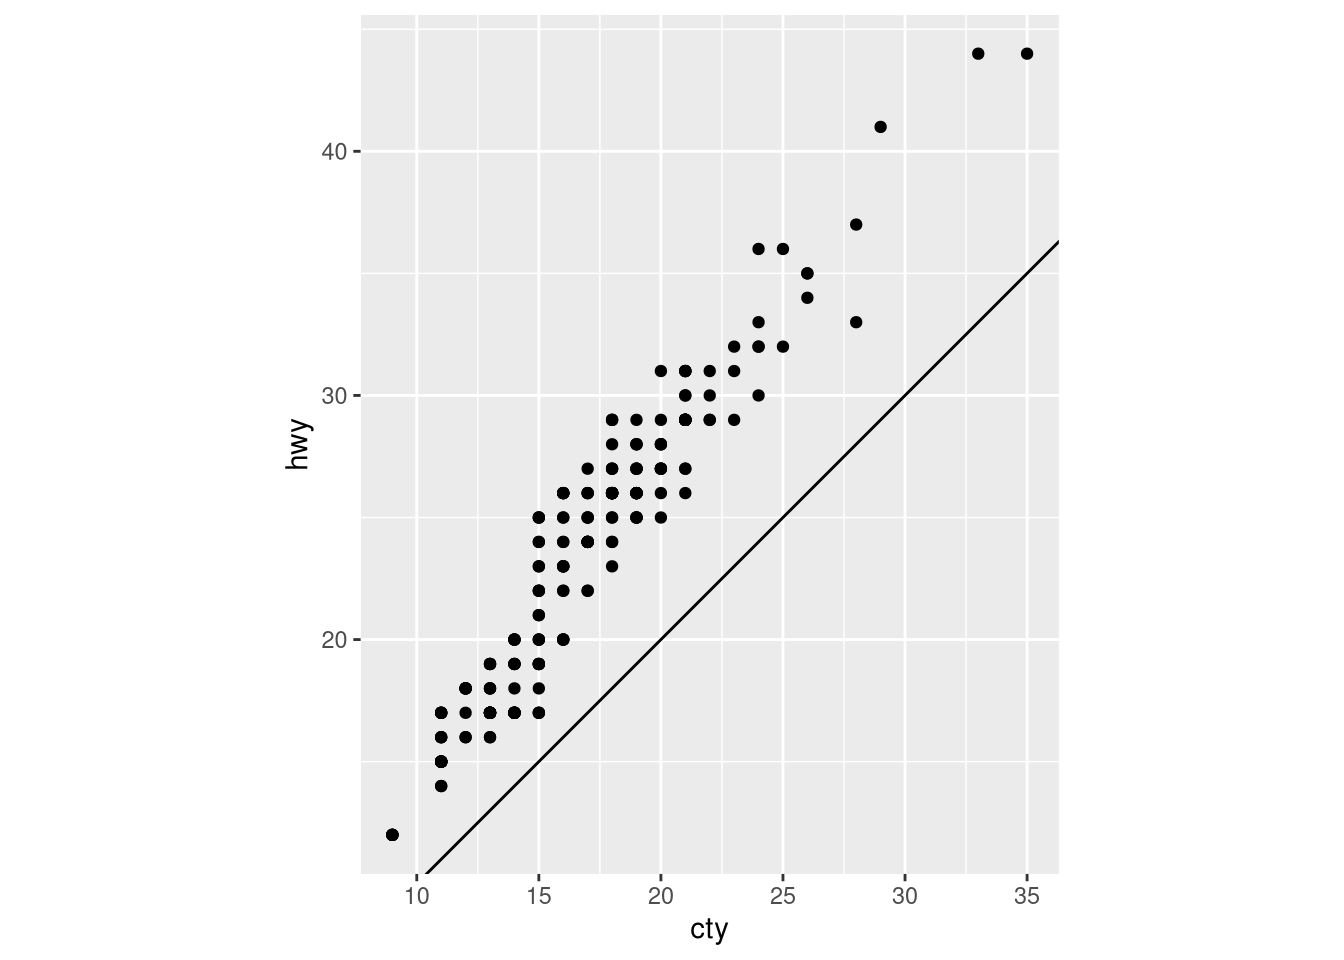
\includegraphics{CH09_files/figure-pdf/unnamed-chunk-41-1.pdf}

  }

  \end{figure}

  \end{tcolorbox}
\end{enumerate}



\end{document}
